% !TEX program = xelatex
% ===========================================================================
% 格点 QCD 计算质子中胶子 PDF 的理论解析与工作流
% 编译: xelatex 理论解析与工作流.tex
% ===========================================================================
\documentclass[11pt,a4paper]{ctexart}

% --------------- 页面设置 ---------------
\usepackage[margin=2.5cm]{geometry}
\usepackage{setspace}
\onehalfspacing

% --------------- 数学与物理 ---------------
\usepackage{amsmath,amssymb,amsfonts}
\usepackage{bm}
\usepackage{braket}
\usepackage{slashed}

% --------------- 图形与颜色 ---------------
\usepackage{graphicx}
\usepackage{xcolor}
\usepackage{tikz}
\usetikzlibrary{arrows.meta, positioning, shapes, decorations.pathmorphing}

% --------------- 表格 ---------------
\usepackage{array,booktabs,multirow}

% --------------- 超链接 ---------------
\usepackage[hidelinks]{hyperref}

% --------------- 代码 ---------------
\usepackage{listings}
\lstset{
  basicstyle=\ttfamily\small,
  breaklines=true,
  frame=single,
  numbers=left,
  numberstyle=\tiny,
  commentstyle=\color{gray},
  keywordstyle=\color{blue},
  stringstyle=\color{red},
}

% --------------- 自定义命令 ---------------
\newcommand{\Fmunu}{F_{\mu\nu}}
\newcommand{\Ftmunu}{\tilde{F}_{\mu\nu}}
\newcommand{\Ftzmu}{\tilde{F}^{\mu z}}
\newcommand{\eps}{\varepsilon}
\newcommand{\LaMET}{\text{LaMET}}
\newcommand{\MSbar}{$\overline{\text{MS}}$}
\newcommand{\QCD}{\text{QCD}}
\newcommand{\tr}{\operatorname{Tr}}
\newcommand{\diag}{\operatorname{diag}}
\newcommand{\vev}[1]{\langle #1 \rangle}
\newcommand{\abs}[1]{|#1|}
\newcommand{\order}[1]{\mathcal{O}(#1)}

% --------------- 标题 ---------------
\title{\textbf{格点 QCD 计算质子中胶子 PDF 的理论解析与工作流}}
\author{基于 donghx 原始代码的系统化理论整理}
\date{2026年7月9日}

\begin{document}

\maketitle

\begin{abstract}
\noindent
本文系统阐述采用大动量有效理论（\LaMET）在格点 QCD 框架下计算质子中非极化胶子部分子分布函数（gluon PDF）的完整理论框架和计算工作流。核心思路是：利用 disconnect 图的因子化性质，将包含胶子算符的三点关联函数解耦为质子两点函数（用 momentum-smeared distillation 计算）和纯规范场的 OPE 算符期望值（Eq.~(25)），然后通过关联函数比提取坐标空间矩阵元（Eq.~(20)），最后经 Fourier 变换和微扰匹配得到光锥 PDF $g(x,\mu)$。文中给出了从格点离散化、Clover 场强张量构造、Wilson 线连接、Distillation 收缩到 quasi-PDF 重构和匹配核卷积的完整推导与算法描述。
\end{abstract}

\tableofcontents
\newpage

% ===========================================================================
\section{QCD与格点规范场理论基础}
% ===========================================================================

在开始讨论大动量有效理论之前，我们需要建立格点QCD的基本理论框架。本节概述连续时空中的QCD拉格朗日量、路径积分量子化方法，以及如何在离散化的欧几里得时空格点上实现非微扰计算。

\subsection{QCD的拉格朗日量与规范对称性}

量子色动力学（QCD）是描述强相互作用的规范场论，其基本自由度是夸克场 $\psi_f(x)$（味指标 $f = u, d, s, c, b, t$）和胶子场 $A_\mu^a(x)$（色指标 $a = 1,\ldots,8$）。连续时空中的QCD拉格朗日量具有 SU(3) 规范对称性：

\begin{equation}
\mathcal{L}_{\text{QCD}} = -\frac{1}{4} F_{\mu\nu}^a F^{a,\mu\nu} + \sum_f \bar{\psi}_f (i\gamma^\mu D_\mu - m_f) \psi_f
\end{equation}

其中胶子场强张量定义为：
\begin{equation}
F_{\mu\nu}^a = \partial_\mu A_\nu^a - \partial_\nu A_\mu^a + g_0 f^{abc} A_\mu^b A_\nu^c
\end{equation}

协变导数为 $D_\mu = \partial_\mu + i g_0 A_\mu^a T^a$，$T^a = \lambda^a/2$ 是 SU(3) 生成元，满足对易关系 $[T^a, T^b] = i f^{abc} T^c$。规范变换下场的变换规律为：
\begin{align}
\psi(x) &\to \Omega(x) \psi(x), \quad \Omega(x) = \exp(i \theta^a(x) T^a) \in \text{SU}(3) \\
A_\mu(x) &\to \Omega(x) A_\mu(x) \Omega^\dagger(x) + \frac{i}{g_0} \Omega(x) \partial_\mu \Omega^\dagger(x)
\end{align}

QCD的两个核心物理特征——\textbf{渐近自由}（高能标下耦合常数变小）和\textbf{色禁闭}（低能标下色荷被束缚在无色的强子中）——使其低能行为必须采用非微扰方法处理。

\subsection{路径积分量子化}

在路径积分表述中，物理观测量 $\mathcal{O}$ 的期望值由泛函积分给出：
\begin{equation}
\langle \mathcal{O} \rangle = \frac{1}{Z} \int \mathcal{D}A_\mu \mathcal{D}\bar{\psi} \mathcal{D}\psi \; \mathcal{O}[A,\bar{\psi},\psi] \; e^{i S_{\text{QCD}}[A,\bar{\psi},\psi]}
\end{equation}
其中配分函数 $Z = \int \mathcal{D}A_\mu \mathcal{D}\bar{\psi} \mathcal{D}\psi \; e^{i S_{\text{QCD}}}$，$S_{\text{QCD}} = \int \mathrm{d}^4 x \, \mathcal{L}_{\text{QCD}}$。

通过 Wick 转动 $t \to -i\tau$（即 $x_0 \to -i x_4$），将 Minkowski 时空转到 Euclidean 时空。此时路径积分中的振荡因子 $e^{iS}$ 变为指数衰减因子 $e^{-S_E}$（$S_E$ 为 Euclidean 作用量），使被积函数变为正定概率权重：
\begin{equation}
\langle \mathcal{O} \rangle_E = \frac{1}{Z_E} \int \mathcal{D}A_\mu \mathcal{D}\bar{\psi} \mathcal{D}\psi \; \mathcal{O}_E \; e^{-S_E[A,\bar{\psi},\psi]}
\end{equation}

这一变换是格点QCD数值模拟的基础——$e^{-S_E}$ 可以解释为统计力学中的 Boltzmann 权重，允许我们使用 Monte Carlo 方法采样规范组态。

\subsection{格点规范理论}

\subsubsection{Wilson规范作用量}

格点QCD在离散的 Euclidean 时空格点上定义理论。设格距为 $a$，格点坐标为 $x = an$，$n=(n_1,n_2,n_3,n_4) \in \mathbb{Z}^4$。基本规范自由度由连接 $x$ 到 $x+a\hat{\mu}$ 的\textbf{规范链接} $U_\mu(x)$ 表示：
\begin{equation}
U_\mu(x) = \mathcal{P} \exp\!\left( i g_0 \int_{x}^{x+a\hat{\mu}} \mathrm{d}y \, A_\mu(y) \right) \in \text{SU}(3)
\end{equation}
其中 $\mathcal{P}$ 为路径排序算符。

最基本的规范不变量是 $1\times 1$ \textbf{Wilson 方格 (plaquette)}：
\begin{equation}
U_{\mu\nu}(x) = U_\mu(x) U_\nu(x+a\hat{\mu}) U_\mu^\dagger(x+a\hat{\nu}) U_\nu^\dagger(x)
\end{equation}

Wilson 规范作用量通过对所有方格求和构造：
\begin{equation}
S_G[U] = \frac{\beta}{3} \sum_x \sum_{\mu<\nu} \operatorname{Re} \operatorname{Tr}[1 - U_{\mu\nu}(x)]
\end{equation}
其中 $\beta = 6/g_0^2$。在 $a \to 0$ 的极限下，该作用量恢复为连续 Yang-Mills 作用量：
\begin{equation}
S_G = \frac{1}{2g_0^2} \sum_x a^4 \operatorname{Tr}[F_{\mu\nu} F^{\mu\nu}] + \order{a^2}
\end{equation}

\subsubsection{费米子作用量与Clover改进}

将连续费米子作用量离散化时，朴素离散化会导致\textbf{fermion doubling}问题（每个连续费米子产生16个格点费米子模式）。Wilson 通过添加量纲为5的项（Wilson项）消除了加倍子，代价是破缺了手征对称性：
\begin{equation}
S_F^{\text{Wilson}} = a^4 \sum_x \bar{\psi}(x) \left( \sum_\mu \gamma_\mu \tilde{\nabla}_\mu - \frac{a r}{2} \sum_\mu \nabla_\mu^* \nabla_\mu + m_0 \right) \psi(x)
\end{equation}
其中 $\tilde{\nabla}_\mu$ 是对称格点导数，$\nabla_\mu^*\nabla_\mu$ 是格点 Laplace 算符。

Wilson 费米子的截断误差为 $\order{a}$。通过添加\textbf{Sheikholeslami-Wohlert (Clover) 项}可以实现 $\order{a}$ 改进：
\begin{equation}
S_F^{\text{Clover}} = S_F^{\text{Wilson}} - a^4 \frac{c_{\text{SW}} r}{4} \sum_x \bar{\psi}(x) \sigma_{\mu\nu} \hat{F}_{\mu\nu}(x) \psi(x)
\end{equation}
其中 $\sigma_{\mu\nu} = \frac{i}{2}[\gamma_\mu, \gamma_\nu]$，$\hat{F}_{\mu\nu}$ 是格点上的场强张量（其 Clover 构造将在第2节详细讨论），$c_{\text{SW}}$ 是改进系数（可在微扰理论或非微扰上确定）。

\subsubsection{连续极限与标度设定}

格点QCD计算的最终目标是提取连续物理（$a \to 0$）。物理观测量在有限格距下具有截断误差：
\begin{equation}
\mathcal{O}^{\text{lat}}(a) = \mathcal{O}^{\text{phys}} + c_1 a^n + c_2 a^{n+1} + \cdots
\end{equation}
其中 $n=1$（未改进）或 $n=2$（$\order{a}$ 改进后）。

标度设定通过选择一个（或多个）实验已知的物理量来确定格距 $a$：
\begin{equation}
a^{-1}(\beta) = \frac{\mathcal{O}^{\text{exp}}}{\mathcal{O}^{\text{lat}}(\beta)}
\end{equation}
常用的标度设定量包括 Wilson 流参数 $w_0$、重正子质量 $M_\Omega$、$\pi$ 介子衰变常数 $f_\pi$ 等。

\subsection{强子谱学与关联函数}

格点QCD中的强子质量通过两点关联函数的大时间行为提取。对于强子插值算符 $\mathcal{O}_H(\mathbf{x}, t)$（具有所需量子数），两点关联函数为：
\begin{equation}
C_2(t) = \sum_{\mathbf{x}} \langle \mathcal{O}_H(\mathbf{x}, t) \mathcal{O}_H^\dagger(\mathbf{0}, 0) \rangle
\end{equation}

插入完备的哈密顿量本征态集合后：
\begin{equation}
C_2(t) = \sum_n |\bra{0} \mathcal{O}_H \ket{n}|^2 e^{-E_n t}
\end{equation}

在大时间极限下，基态占主导：
\begin{equation}
C_2(t) \xrightarrow{t \to \infty} |Z_0|^2 e^{-E_0 t}
\end{equation}

由此可以提取强子质量 $E_0 = m_H$（静止系）或 $E_0 = \sqrt{m_H^2 + \mathbf{P}^2}$（运动系）。

在实际计算中，为了增强基态重叠并压制 UV 涨落，需要对夸克场进行\textbf{涂抹}（smearing）。常用的涂抹方法包括 Jacobi 涂抹、Wuppertal 涂抹和 Distillation（将在第4节详细讨论）。

\subsection{夸克传播子与关联函数的计算}

\subsubsection{夸克传播子}

夸克传播子定义为 Dirac 算符的逆：$S(x,y) = D^{-1}(x,y)$。在实际计算中，对于给定的源 $\eta(y)$，通过求解线性系统得到解 $\psi(x)$：
\begin{equation}
\sum_y D(x,y) \psi(y) = \eta(x), \quad \psi(x) = \sum_y S(x,y) \eta(y)
\end{equation}

通常使用共轭梯度（CG）类迭代求解器，收敛速率由 Dirac 算符的条件数决定——该条件数在接近手征极限（$m_q \to 0$）时发散，导致\textbf{临界减速}现象。

\subsubsection{点源与涂抹源}

最简单的源是\textbf{点源}：$\eta(y) = \delta_{y,y_0} \delta_{\alpha\alpha_0} \delta_{aa_0}$，但点源与强子基态的重叠很差。涂抹源通过在空间上扩展源来增强与物理态的耦合。常用的涂抹源包括：
\begin{itemize}
  \item \textbf{Wall 源}：在固定时间片上，所有空间点取常数值（需要规范固定）；
  \item \textbf{Gaussian 源}：$\eta(x) \propto \exp(-|\mathbf{x} - \mathbf{x}_0|^2 / (2\sigma^2))$；
  \item \textbf{Jacobi 涂抹源}：通过迭代应用规范协变的 hopping 算符构建。
\end{itemize}

\subsubsection{夸克场双线性算符的 Wick 收缩}

对于形如 $\bar{\psi}(x) \Gamma \psi(x)$ 的定域夸克双线性算符，Wick 收缩给出：
\begin{equation}
\contraction{}{\bar{\psi}}{(x) \Gamma}{\psi}
\bar{\psi}(x) \Gamma \psi(x) \to -\tr[\Gamma S(x,x)]
\end{equation}

对于非定域的双线性（如 $\bar{\psi}(x) \Gamma W(x,y) \psi(y)$），收缩涉及从 $y$ 到 $x$ 的夸克传播子，中间插入 Wilson 线。

\subsection{格点QCD数值模拟的基本流程}

完整的格点QCD数值模拟包括以下步骤：
\begin{enumerate}
  \item \textbf{规范组态生成}：使用 HMC (Hybrid Monte Carlo) 算法对 SU(3) 规范场采样，生成具有概率权重 $e^{-S_E[U]}$ 的规范组态系综；
  \item \textbf{夸克传播子计算}：在固定规范组态上，通过求解 Dirac 方程 $D[U] \psi = \eta$（$\eta$ 为点源或涂抹源）得到夸克传播子；
  \item \textbf{Wick 收缩}：将夸克传播子按照 Wick 定理收缩为所需的强子关联函数；
  \item \textbf{统计分析与物理提取}：对组态系综求平均，利用拟合方法提取物理观测量（质量、矩阵元等），并进行连续极限和手征外推。
\end{enumerate}

本节建立的理论基础为后续讨论格点胶子 PDF 计算提供了必要的背景知识。接下来我们进入大动量有效理论（\LaMET）的核心内容。

% ===========================================================================
\section{理论基础}
% ===========================================================================

\subsection{光锥 PDF 的定义与物理起源}

\subsubsection{从深度非弹性散射到部分子分布}

部分子分布函数（PDF）的概念起源于对深度非弹性散射（DIS）实验的描述。在 DIS 过程 $e + p \to e + X$ 中，高能电子通过交换虚光子 $\gamma^*$ 来探测质子的内部结构。DIS 的双微分截面为：
\begin{equation}
\frac{\mathrm{d}^2\sigma}{\mathrm{d}x_{\text{B}} \mathrm{d}Q^2} = \frac{4\pi\alpha^2}{x_{\text{B}} Q^4} \left[ \left(1 - y + \frac{y^2}{2}\right) F_2(x_{\text{B}}, Q^2) - \frac{y^2}{2} F_L(x_{\text{B}},Q^2) \right]
\end{equation}
其中 $x_{\text{B}} = Q^2/(2P\cdot q)$ 为 Bjorken-$x$，$Q^2 = -q^2$ 为虚光子动量平方，$y = P\cdot q/(P\cdot k)$ 为非弹性度。

在 Bjorken 极限下（$Q^2 \to \infty$，$x_{\text{B}}$ 固定），结构函数 $F_2$ 呈现近似标度无关性（Bjorken scaling）。根据 QCD 因子化定理，结构函数可以因子化为硬散射截面（可微扰计算）与 PDF（非微扰）的卷积：
\begin{equation}
F_2(x_{\text{B}}, Q^2) = \sum_{a=q,\bar{q},g} \int_{x_{\text{B}}}^{1} \frac{\mathrm{d}z}{z} \,
C_{2,a}\!\left(\frac{x_{\text{B}}}{z}, \frac{Q^2}{\mu^2}, \alpha_s(\mu)\right) f_a(z, \mu^2)
\end{equation}
其中 $f_a(x, \mu^2)$ 是味为 $a$ 的部分子携带纵向动量分数 $x$ 的概率密度，$C_{2,a}$ 是硬散射系数函数。

\subsubsection{光锥关联函数定义}

在 QCD 的算符形式中，部分子分布可以通过光锥关联函数的 Fourier 变换严格定义。对于质子中的非极化胶子，其光锥 PDF $g(x,\mu^2)$ 定义为：
\begin{equation}\label{eq:lightcone_pdf}
g(x, \mu^2) = \int \frac{\mathrm{d}\xi^{-}}{2\pi x P^{+}} \,
e^{-i x P^{+}\xi^{-}} \,
\braket{P | F^{+\mu}(\xi^{-}) \, W(\xi^{-}, 0) \, \tilde{F}_{\mu}^{\;+}(0) | P}
\end{equation}
其中：
\begin{itemize}
  \item $P^{+} = (P^{0} + P^{3})/\sqrt{2}$ 为光锥坐标下的正向动量；
  \item $\Fmunu$ 为胶子场强张量，$F^{+\mu}$ 为其在 $+$ 方向上的分量；
  \item $\Ftmunu = \tfrac{1}{2}\eps_{\mu\nu\rho\sigma}F^{\rho\sigma}$ 为对偶场强张量；
  \item $W(\xi^{-},0)$ 为连接 $\xi^{-}$ 与 $0$ 的光锥 Wilson 线，确保关联函数的规范不变性：
  \begin{equation}
  W(\xi^{-}, 0) = \mathcal{P} \exp\!\left( i g_0 \int_{0}^{\xi^{-}} \mathrm{d}\eta^{-} A^{+}(\eta^{-}) \right)
  \end{equation}
  \item $x$ 为 Bjorken-$x$（胶子携带的纵向动量分数）；
  \item $\mu$ 为重整化标度，PDF 通过 DGLAP 方程依赖于 $\mu$。
\end{itemize}

光锥关联函数定义在等光锥时间 $\xi^{+} = 0$ 的超曲面上，这就要求理论是 Minkowski 度规的。这正是在 Euclidean 格点上直接计算光锥 PDF 的根本困难所在。

\subsubsection{Twist展开与Leading-Twist近似}

光锥关联函数可以在 twist 展开的框架下系统分类。算符的 twist 定义为质量量纲减去自旋：$\tau = d - s$。对于 PDF，leading-twist（$\tau = 2$）贡献来自光锥上算符乘积展开的主导项，高 twist（$\tau \geq 3$）修正被 $1/Q^2$ 幂次压低。

胶子 PDF 的 twist-2 算符就是上述光锥关联函数~\eqref{eq:lightcone_pdf} 的被积函数。对于非极化情形，在光锥规范 $A^{+}=0$ 下，Wilson 线化为单位矩阵，关联函数简化为：
\begin{equation}
\braket{P | F^{+\mu}(\xi^{-}) \, \tilde{F}_{\mu}^{\;+}(0) | P}_{A^{+}=0}
\end{equation}

\subsubsection{动量求和规则}

胶子 PDF 与夸克 PDF 通过动量求和规则相互关联，反映了强子总动量的守恒：
\begin{equation}
\int_{0}^{1} \mathrm{d}x \, x \left[ \sum_{f} (q_f(x,\mu^2) + \bar{q}_f(x,\mu^2)) + g(x,\mu^2) \right] = 1
\end{equation}
实验数据显示，在 $\mu^2 \sim 10\;\text{GeV}^2$ 的标度下，胶子携带约 40--45\% 的质子动量，这使得胶子 PDF 的精确计算对理解质子结构至关重要。

\subsection{大动量有效理论（\LaMET）}

\subsubsection{Feynman部分子模型与无穷动量框架}

部分子物理学的现代理解始于 Feynman 的部分子模型：在高能散射中，快速运动的强子可以视为一束近乎自由的、无相互作用的部分子（夸克和胶子），每个部分子携带强子纵向动量的一部分 $x = k_z/P_z$。这一图景在无穷动量框架（Infinite Momentum Frame, IMF）中最为清晰，即 $P_z \to \infty$。

从 Weinberg 的无穷动量微扰理论角度，在 IMF 中 QCD 的真空简化，强子态可以展开为自由 Fock 空间中的多部分子态。然而，IMF 形式化存在数学困难：无穷大动量和 UV 截断的极限不可交换。

\LaMET{} 通过将 IMF 替换为有限但足够大的动量 $P_z$ 来解决这一困难，与重夸克有效理论（HQET）将无穷大夸克质量替换为有限大夸克质量的策略完全类似。

\subsubsection{LaMET与HQET的类比}

HQET 和 LaMET 都是处理含有一个大标度的物理系统的有效场论方法：
\begin{center}
\begin{tabular}{c|c|c}
\toprule
\textbf{特征} & \textbf{HQET} & \textbf{LaMET} \\
\midrule
大标度 & 重夸克质量 $m_Q$ & 强子动量 $P_z$ \\
展开参数 & $1/m_Q$ & $1/P_z$ \\
有效理论 & HQET 拉格朗日量 & 部分子模型/光锥关联 \\
匹配因子 & $Z(m_Q/\Lambda, \Lambda/\mu)$ & $Z(P_z/\Lambda, \Lambda/\mu)$ \\
幂次修正 & $\order{1/m_Q}$ & $\order{\Lambda_{\text{QCD}}^2/P_z^2}$ \\
\bottomrule
\end{tabular}
\end{center}

在 HQET 中，包含重夸克的物理观测量 $O(m_Q)$ 在大质量极限下展开为：
\begin{equation}
O(m_Q/\Lambda) = Z(m_Q/\Lambda, \Lambda/\mu) \, o(\mu) + \order{1/m_Q} + \cdots
\end{equation}
其中 $o(\mu)$ 是 HQET 中的算符矩阵元，$Z$ 是微扰可计算的匹配系数。

类似地，在 LaMET 中，格点上依赖于大动量 $P_z$ 的观测量 $F(P_z/\Lambda)$ 在大动量极限下展开为：
\begin{equation}\label{eq:lamet_expansion}
F(P_z/\Lambda) = Z(P_z/\Lambda, \Lambda/\mu) \, f(\mu) + \order{\frac{\Lambda_{\text{QCD}}^{2}}{P_z^{2}}}
\end{equation}
其中 $f(\mu)$ 是 $P_z \to \infty$ 时的光锥观测量（即部分子分布），包含所有红外共线奇点。这意味着，\textbf{Feynman的部分子模型实际上就是大动量强子的有效理论}！

\subsubsection{因子化定理的形式推导}

对于任意依赖于大动量 $P_z$ 的 Euclidean 观测量 $F(P_z/\Lambda, \Lambda/\mu)$，在固定格距的格点上计算 $F$ 时，先取 $a \to 0$ 得到连续极限，再在 $P_z \gg \Lambda_{\text{QCD}}$ 的条件下展开。展开的系统性来自于渐近自由：当 $P_z$ 很大时，$F$ 对 $P_z$ 的依赖是可微扰计算的。

因子化公式~\eqref{eq:lamet_factorization} 中的匹配核 $C$ 的独立变元为 $x/y$ 和 $\mu/(yP_z)$（注意：不是 $\mu/P_z$，而是 $\mu/(yP_z)$——匹配核依赖于部分子动量 $yP_z$ 而非强子动量 $P_z$，这一重要的精细区别由 Izubuchi、Ji 等人于 2018 年阐明）：
\begin{equation}\label{eq:lamet_factorization_corrected}
\tilde{q}(x, P_z) = \int_{-1}^{1} \frac{\mathrm{d}y}{|y|} \,
C\!\left(\frac{x}{y}, \frac{\mu}{|y|P_z}\right) \,
q(y, \mu) + \order{\frac{\Lambda_{\text{QCD}}^{2}}{P_z^{2}},\;
\frac{\Lambda_{\text{QCD}}^{2}}{x^{2}P_z^{2}}}
\end{equation}

\subsubsection{幂次修正的系统分析}

LaMET 的幂次修正来自多个来源：

\begin{enumerate}
  \item \textbf{靶质量修正}：有限质子质量 $M_N$ 导致的修正，量级为 $\order{M_N^2/P_z^2}$；
  \item \textbf{高 twist 修正}：量级为 $\order{\Lambda_{\text{QCD}}^2/P_z^2}$，来自 twist-4 及更高 twist 算符的贡献；
  \item \textbf{小 $x$ 区域的增强修正}：量级为 $\order{\Lambda_{\text{QCD}}^2/(x^2 P_z^2)}$，当 $x$ 很小时这些修正被放大。
\end{enumerate}

对于典型的格点动量 $P_z \sim 1.5\text{--}2.5$ GeV 和 $\Lambda_{\text{QCD}} \sim 0.3$ GeV，幂次修正的量级约为 $(\Lambda_{\text{QCD}}/P_z)^2 \sim 1.5\%\text{--}4\%$，表明即使在中等动量下 LaMET 的收敛性也是可接受的。

\textbf{收敛性判据}：对于可信的 PDF 提取，需要 $P_z \gtrsim 1.5$ GeV 且 $x P_z \gg \Lambda_{\text{QCD}}$（后者排除了非常小的 $x$ 区域）。

\subsubsection{大动量重整化群方程}

匹配因子 $Z(P_z/\Lambda, \Lambda/\mu)$ 满足重整化群方程。定义反常维数：
\begin{equation}
\gamma(\alpha_s) = \frac{1}{Z} \frac{\partial Z}{\partial \ln P_z}
\end{equation}
则准观测量满足：
\begin{equation}
\frac{\partial F(P_z)}{\partial \ln P_z} = \gamma(\alpha_s) F(P_z) + \order{\frac{1}{P_z^{2}}}
\end{equation}
利用这一方程可以对 $P_z$ 的大对数进行重求和，提高微扰匹配的精度。

\subsubsection{从Euclidean关联到Minkowski光锥关联的解析延拓}

LaMET 的一个关键理论要素是证明 Euclidean 格点计算能够捕获正确的 Minkowski 光锥物理。这通过解析延拓实现：Euclidean 圈积分在解析延拓 $p_\tau \to -i p_0$ 后精确地重现 Minkowski 圈积分的红外共线发散结构。具体来说，考虑一个典型的单圈 Feynman 积分，Minkowski 版本 $I_M$ 具有共线发散（当部分子质量 $m \to 0$ 时），而 Euclidean 版本 $I_E$ 在解析延拓后满足 $I'_E = -i I_M$。这证明了：\textbf{格点 QCD 在有限 $P_z$ 下计算的非局域关联函数包含了与光锥 PDF 相同的红外物理}，两者的差异仅在于 UV 区域，这可以通过微扰匹配核来弥补。

\subsection{准 PDF 与匹配关系}

\subsubsection{从 Euclidean 关联函数到 quasi-PDF}

对于胶子 quasi-PDF，取 $z$ 方向为 boost 方向，空间方向的 quasi-PDF 定义为：
\begin{equation}\label{eq:quasi_pdf_def}
\tilde{g}(x, P_z) = \int \frac{\mathrm{d}z}{2\pi x P_z} \,
e^{i x P_z z} \, \tilde{h}(z, P_z)
\end{equation}
其中\textbf{坐标空间矩阵元} $\tilde{h}(z, P_z)$ 为：
\begin{equation}\label{eq:matrix_element}
\boxed{\tilde{h}(z, P_z) = \frac{\braket{P | O(z) | P}}{\braket{P|P}}}
\end{equation}
这就是 Note 中 \textbf{Eq.~(20)} 的核心内容。

\textbf{推导要点}：上述 Fourier 变换关系来自将光锥关联函数中沿光锥方向 $\xi^-$ 的积分替换为沿空间方向 $z$ 的积分。在 IMF 中，Lorentz 收缩效应使得 $\xi^- \sim z/\gamma$（其中 $\gamma = P_z/M$），因此需要乘以 Jacobian 因子 $1/(xP_z)$。

\subsubsection{因子化定理的算符乘积展开推导}

准 PDF 到光锥 PDF 的匹配关系可以通过算符乘积展开（OPE）严格推导。考虑坐标空间中的重正化 Wilson 算符 $O(z, \mu)$，在短距离极限 $z \to 0$ 下，其 OPE 展开为：
\begin{equation}
O(z, \mu) = \sum_n C_n(\mu^2 z^2) \, \frac{(-iz)^n}{n!} \,
e_{\mu_1}\cdots e_{\mu_n} \, \mathcal{O}_n^{\mu_1\cdots\mu_n}(\mu) + \cdots
\end{equation}
其中 $\mathcal{O}_n$ 是 twist-2 的定域算符，Wilson 系数 $C_n$ 在 $\overline{\text{MS}}$ 方案下微扰可计算。这一展开表明，非定域算符的短距离行为完全由定域 twist-2 算符决定，而后者正是 PDF 的 Mellin 矩的来源。

\subsubsection{准 PDF 与赝 PDF 的等价性}

除了通过 Fourier 变换定义 quasi-PDF 外，还有一种等价的途径——\textbf{赝 PDF (pseudo-PDF)} 方法。赝 PDF 直接在 Ioffe 时间 $\nu = z P_z$ 中工作：
\begin{equation}
\mathcal{P}(x, z^2) = \int \frac{\mathrm{d}\nu}{2\pi} \, e^{-i x \nu} \,
\tilde{h}(\nu, z^2)
\end{equation}
其中 $\tilde{h}(\nu, z^2)$ 是 Lorentz 不变的 Ioffe 时间分布。准 PDF 和赝 PDF 是\textbf{同一空间关联函数}的两种不同表示——分别对应 Fourier 变换到 $x P_z$ 空间和 $\nu = z P_z$ 空间。它们在数学上完全等价，匹配系数可通过变量替换相互转换：
\begin{center}
\begin{tabular}{c|c|c}
\toprule
\textbf{分布} & \textbf{Fourier 变换} & \textbf{参量} \\
\midrule
空间关联 & --- & $\zeta = zP_z$, $z^2$ \\
准 PDF (quasi-PDF) & $z \to xP_z$ & $x$, $P_z$ \\
赝 PDF (pseudo-PDF) & $\zeta \to x$ & $x$, $z^2$ \\
\bottomrule
\end{tabular}
\end{center}

\subsubsection{NLO 匹配核}

quasi-PDF 到光锥 PDF 的 NLO 匹配关系为（$\mu$ 为 \MSbar{}标度）：
\begin{equation}
\tilde{g}(x, P_z) = g(x, \mu) + \frac{\alpha_s}{2\pi}
\int_{x}^{1} \frac{\mathrm{d}y}{y} \,
\Delta C_{gg}\!\left(\frac{x}{y}, \frac{\mu}{P_z}\right) g(y, \mu) + \cdots
\end{equation}

对于胶子，NLO 匹配核 $\Delta C_{gg}$ 包含以下结构：
\begin{itemize}
  \item \textbf{LO（树图）}：$C_{gg}^{(0)}(\xi) = \delta(1-\xi)$；
  \item \textbf{NLO}：包含 $1/(1-\xi)_+$ 型的 plus-distribution、$\delta(1-\xi)$ 项，以及 $\ln(\mu^2/P_z^2)$ 对数项；
  \item \textbf{大 $x$ 区域}：当 $\xi \to 1$ 时，出现大的对数 $\ln(1-\xi)$，需要通过阈值重求和来恢复微扰收敛性。
\end{itemize}

Matching kernel 的完整 NLO 表达式将在第 5 节详细讨论。重要的是，匹配核 $C_{gg}(x/y, \mu/P_z)$ 仅依赖于部分子动量比 $x/y$ 和标度比 $\mu/P_z$，与外部强子态无关——这是因子化定理的核心结论。

\subsubsection{NLO 匹配的数值意义}

为了理解 NLO 匹配修正的大小，考虑在典型标度下的数值估计。取 $\alpha_s(\mu=2\;\text{GeV}) \approx 0.25$，匹配修正量级约为 $\alpha_s/(2\pi) \sim 4\%$。在中等 $x$ 区域（$0.1 < x < 0.5$），匹配修正是可控的微扰修正；在大 $x$ 区域，阈值对数 $\ln(1-x)$ 可能增强修正，需谨慎处理；在小 $x$ 区域，$1/x$ 型的增强可能也需要重求和。

\subsection{胶子 quasi-PDF 算符}

\subsubsection{非极化胶子算符}

胶子 unpolarized quasi-PDF 算符在空间方向上的定义为：
\begin{equation}
O_{\mu\nu}(z) \equiv F_{z\mu}(z\hat{n}_z) \; W(z\hat{n}_z, 0) \; \tilde{F}_{\nu}^{\;z}(0)
\end{equation}
其中 $\hat{n}_z$ 是空间 $z$ 方向的单位矢量。

对于 unpolarized 情形，需要的指标收缩为：
\begin{equation}\label{eq:ope_unpol}
\boxed{O(z) = O_{\mu}^{\;\mu}(z) = F_{z\mu}(z) \, W(z, 0) \, \tilde{F}^{\mu z}(0)}
\end{equation}

\textbf{Eq.~(25)} 给出了我们具体拆解出的 OPE 算符形式——用 $F$ 和 $\tilde{F}$ 的不同 Lorentz 分量组合。在格点计算中，由于旋转对称性破缺，需要对等价方向进行平均。以 $z$ 方向 boost 为例，横向指标 $\mu \in \{x, y, t\}$ 需独立求和：
\begin{equation}
O_{\text{unpol}}(z) \equiv \sum_{\mu \neq z}
\Bigl[ F_{z\mu}(z) \, W(z, 0) \, \Ftzmu(0) \Bigr]_{\text{对称化}}
\end{equation}

\subsubsection{极化与非极化胶子算符的区别}

胶子 PDF 的极化态由场强张量的不同缩并方式来区分。对于\textbf{螺旋度（极化）胶子 PDF} $\Delta g(x, \mu^2)$，算符中的 $\tilde{F}^{\mu z}$ 被替换为 $F^{\mu z}$（即不使用对偶张量），二者之差对应对偶变换：
\begin{equation}
\Delta O(z) = F_{z\mu}(z) \, W(z,0) \, F^{\mu z}(0) - F_{z\mu}(z) \, W(z,0) \, \tilde{F}^{\mu z}(0)
\end{equation}
极化胶子 PDF 的实验提取对于解决质子自旋危机至关重要——Jaffe-Manohar 自旋分解
$\frac{1}{2} = \frac{1}{2}\Delta\Sigma + \Delta G + L_z$
中的 $\Delta G$ 正是极化胶子 PDF 的一阶矩。

\subsubsection{多重性可重正性与算符混合}

Li、Ma 和 Qiu（2018）证明了：所有 36 个独立的准胶子算符在重整化下是\textbf{可乘可重整的}，且彼此之间不发生混合。这一结论推广了此前对准夸克算符的证明，为从格点 QCD 中提取胶子 PDF 奠定了完整的理论基础。

证明的关键在于：在规范不变的 UV 正规化方案下，所有来自胶子-规范链接顶点的线性 UV 发散在考虑了所有 Feynman 图后相互抵消。这是因为所有 UV 发散都定域在时空中——它们来自圈动量的横向分量趋向无穷大而纵向分离 $|z|$ 很小的区域。

\textbf{对格点计算的启示}：由于不存在算符混合，我们不需要像处理某些夸克算符（如 $\gamma_z$ 准 PDF 与 twist-3 标量算符的混合）那样构造混合矩阵。这简化了胶子 quasi-PDF 的非微扰重整化。

\subsubsection{胶子 quasi-PDF 算符的 Lorentz 分量分类}

在有限格距的格点上，Euclidean 旋转对称性 $O(4)$ 破缺为超立方对称性 $H(4)$。因此，连续理论中由 Lorentz 对称性关联的不同分量在格点上需要独立处理。对于 Wilson 线沿 $z$ 方向的构型，非极化的三个独立分量为：

\begin{center}
\begin{tabular}{c c c c}
\toprule
\textbf{分量} & \textbf{($\mu,\nu$) 组合} & \textbf{物理内容} & \textbf{在连续极限下的贡献} \\
\midrule
电-电 & $(t, x)$ 和 $(t, y)$ & $F_{zt} W \tilde{F}^{tz}$ & $E_\perp \cdot E_\perp$ 型 \\
电-磁 & $(t, x)$ 和 $(t, y)$ 的线性组合 & $F_{zt} W \tilde{F}^{tz}$ 的反对称部分 & --- \\
磁-磁 & $(x, y)$ & $F_{zx} W \tilde{F}^{xz} + F_{zy} W \tilde{F}^{yz}$ & $B_\perp \cdot B_\perp$ 型 \\
\bottomrule
\end{tabular}
\end{center}

在连续极限下，所有三个分量的贡献合并为所需的 Lorentz 不变量。在有限格距下，通过对所有等价方向求平均来部分恢复旋转对称性。

% ===========================================================================
\section{格点离散化}
% ===========================================================================

\subsection{场强张量的格点构造（Clover 定义）}

在格点上，场强张量 $\Fmunu$ 通过规范链接 $U_\mu(x)$ 构造。

\textbf{Plaquette（方格）}在 $\mu$-$\nu$ 平面上的定义为：
\begin{equation}
P_{\mu\nu}(x) = U_\mu(x)\,U_\nu(x+\hat{\mu})\,U_\mu^{\dagger}(x+\hat{\nu})\,U_\nu^{\dagger}(x)
\end{equation}

\textbf{Clover 算符}通过对围绕点 $x$ 的四个 plaquette 取反对称化组合，得到 $\order{a^2}$ 改进的场强张量：
\begin{equation}\label{eq:clover_F}
\hat{F}_{\mu\nu}(x) = -\frac{i}{8a^{2}g_{0}}
\Bigl( Q_{\mu\nu}(x) - Q_{\mu\nu}^{\dagger}(x) \Bigr)
\end{equation}
其中 $Q_{\mu\nu}$ 是 ``clover leaf''——四个 plaquette 之和：
\begin{equation}
Q_{\mu\nu}(x) = P_{\mu\nu}(x) + P_{\nu,-\mu}(x) + P_{-\mu,-\nu}(x) + P_{-\nu,\mu}(x)
\end{equation}

四个 plaquette 的几何排列如图所示（以点 $x$ 为中心）：
\begin{center}
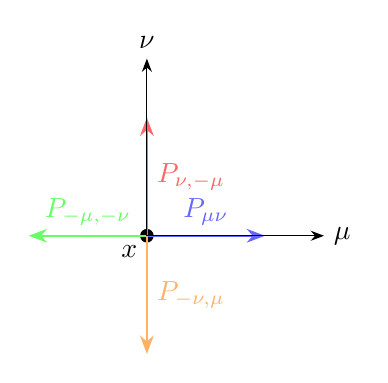
\begin{tikzpicture}[scale=1.5, >=Stealth]
  % 中心点
  \filldraw (0,0) circle (1.5pt) node[below left] {$x$};
  % 四个方向的 plaquette 简化表示
  \draw[->, thick, blue!60] (0,0) -- (1,0) node[midway, above] {$P_{\mu\nu}$};
  \draw[->, thick, red!60] (0,0) -- (0,1) node[midway, right] {$P_{\nu,-\mu}$};
  \draw[->, thick, green!60] (0,0) -- (-1,0) node[midway, above] {$P_{-\mu,-\nu}$};
  \draw[->, thick, orange!60] (0,0) -- (0,-1) node[midway, right] {$P_{-\nu,\mu}$};
  % 坐标轴
  \draw[->] (0,0) -- (1.5,0) node[right] {$\mu$};
  \draw[->] (0,0) -- (0,1.5) node[above] {$\nu$};
\end{tikzpicture}
\end{center}

在代码中取 $a=1$, $g_0=1$，Clover 场强张量为：
\begin{equation}
\hat{F}_{\mu\nu}(x) = -\frac{i}{8} \Bigl[
P_{\mu\nu} + P_{\nu,-\mu} + P_{-\mu,-\nu} + P_{-\nu,\mu}
- \text{h.c.} \Bigr]
\end{equation}

\subsection{对偶场强张量}

对偶场强张量 $\Ftmunu$ 通过 Levi-Civita 张量与 $F$ 联系：
\begin{equation}\label{eq:dual_F}
\Ftmunu = \frac{1}{2}\,\eps_{\mu\nu\rho\sigma}\,F^{\rho\sigma}
\end{equation}
其中 $\eps_{\mu\nu\rho\sigma}$ 是四维完全反对称张量，约定 $\eps_{0123}=+1$。

在代码中，\texttt{Tensor4} 数组实现了 $\tfrac{1}{2}\eps_{\mu\nu\rho\sigma}$：
\begin{equation}
\eps_{\mu\nu\rho\sigma} = \begin{cases}
+1, & (\mu,\nu,\rho,\sigma)\text{ 是 }(0,1,2,3)\text{ 的偶排列},\\
-1, & \text{奇排列},\\
0,  & \text{有重复指标}.
\end{cases}
\end{equation}

\texttt{plaquette\_clover\_all\_tilde} 函数通过缩并实现 $\tilde{F}$：
\begin{lstlisting}[language=Python]
pla_tilde[mu, nu] = contract("opmn, mntzyxab -> optzyxab",
                              epsilon4, pla_all)
\end{lstlisting}

\subsection{Wilson 线}

连接 $0$ 和 $z\hat{n}$ 的 Wilson 线是路径有序指数：
\begin{equation}
W(z\hat{n}, 0) = \mathcal{P} \exp\!\left( i g_0 \int_{0}^{z} \mathrm{d}z' \, A_z(z'\hat{n}) \right)
\end{equation}
在格点上离散化为规范链接的乘积：
\begin{equation}\label{eq:wilson_line}
W(z\hat{n}_z, 0) \;\approx\; \prod_{k=0}^{z/a-1} U_z(k a \hat{n}_z)
\end{equation}

代码中正向 Wilson 线用 $U_z$ 链接连乘，反向（由 $z$ 到 $0$）用 $U_z^{\dagger}$ 连乘：
\begin{lstlisting}[language=Python]
# z -> 0 的 Wilson 线 (取 U_z 的共轭)
for dz in range(delta_z):
    ope = contract("tzyxab, tzyxcb -> tzyxac",
                   ope, gauge[..., z_dir, :, :].conj()[rolled])
# 0 -> z 的 Wilson 线 (U_z 正向)
for dz in range(delta_z):
    ope = contract("tzyxab, tzyxbc -> tzyxac",
                   ope, gauge[..., z_dir, :, :][rolled])
\end{lstlisting}

\subsection{完整胶子算符的格点实现}

完整的 nonlocal 胶子算符 $O_{\mu\nu}(z)$ 的格点表示为：
\begin{equation}\label{eq:full_operator}
\boxed{
O_{\mu\nu}^{\text{lat}}(z) = \tr_c\!\left[
\hat{F}_{z\mu}(z\hat{n}_z) \;
\Bigl( \prod_{k=0}^{z/a-1} U_z(k a) \Bigr) \;
\hat{\tilde{F}}_{\nu}^{\;z}(0) \;
\Bigl( \prod_{k=z/a-1}^{0} U_z^{\dagger}(k a) \Bigr)
\right]
}
\end{equation}

代码中对应 \texttt{operators\_new\_z0\_mu2} 函数的五步构造法：
\begin{enumerate}
  \item 将 $\hat{F}_{\mu\nu}$ (plaquette) 平移到 $z$ 位置；
  \item 从 $z$ 到 $0$ 连接 Wilson 线（$U_z$ 的共轭）；
  \item 在 $0$ 处插入 $\hat{\tilde{F}}_{\mu_2,\nu_2}$；
  \item 从 $0$ 到 $z$ 连接 Wilson 线（$U_z$）；
  \item 对颜色空间取迹 $\tr_c[\cdots]$，对空间求和 $\sum_{x,y}$。
\end{enumerate}

\subsection{Symanzik 改进程序与 $\order{a^2}$ 改进}

\subsubsection{Symanzik 有效作用量方法}

Symanzik 改进程序是系统地消除格点截断误差的方法。核心思想是：格点理论可以视为连续理论的\textbf{有效理论}，其作用量包含高维算符（由高能模的积分产生），这些高维算符被格距 $a$ 的幂次压低：
\begin{equation}
S_{\text{eff}} = S_{\text{cont}} + a \int \mathrm{d}^4 x \, c_1 \mathcal{O}_5(x) + a^2 \int \mathrm{d}^4 x \, c_2 \mathcal{O}_6(x) + \cdots
\end{equation}
通过调节作用量中的参数（改进系数），可以从经典水平或量子水平上消除低阶的截断误差。

\subsubsection{Clover 改进的 $\order{a^2}$ 性质}

我们的胶子算符中使用的 Clover 场强张量构造天然具有 $\order{a^2}$ 改进性质。这是因为：
\begin{enumerate}
  \item Clover 叶由围绕同一点 $x$ 的四个 plaquette 的反对称组合构成，这消除了单个 plaquette 中存在的 $\order{a}$ 误差；
  \item 取反厄米部分 $Q - Q^\dagger$ 进一步消除了无关的色单态贡献；
  \item 四个方向的对称平均恢复了连续极限下的 Lorentz 协变性（在格点上破缺为超立方对称性）。
\end{enumerate}

推广到非定域算符 $O(z)$，由于算符包含 Clover 场强张量和沿直线连接它们的 Wilson 线，Symanzik 分析表明前导离散化误差为 $\order{a^2}$（而非 $\order{a}$）。然而，Wilson 线本身可能引入额外的 $\order{a}$ 效应——这可以通过 HYP 涂抹来缓解。

\subsubsection{Tadpole 改进（平均场改进）}

在格点微扰论中，规范链接 $U_\mu$ 的高阶 tadpole 图贡献大的、纯规范的重整化因子 $u_0$。Lepage 和 Mackenzie 提出的 tadpole 改进通过重新标度链接变量 $U_\mu \to U_\mu/u_0$ 来吸收这些贡献，其中 $u_0$ 可以从 plaquette 的平均值估计：
\begin{equation}
u_0 = \left( \frac{1}{3} \langle \operatorname{Re} \operatorname{Tr} P_{\mu\nu} \rangle \right)^{1/4}
\end{equation}
虽然我们的胶子算符计算中取 $a=1, g_0=1$（即已吸收到归一化中），但在比较不同格距的绝对归一化时需要考虑 tadpole 改进。

\subsection{HYP 涂抹与 Wilson 线的改进}

\subsubsection{HYP 涂抹的动机}

格点上的 Wilson 线 $W(z,0) = \prod_{k=0}^{z/a-1} U_z(k a)$ 是裸规范链接的乘积。裸链接包含大量 UV 涨落，导致：
\begin{enumerate}
  \item 大的统计噪声（特别是长 Wilson 线）；
  \item 强的线性发散 $\propto |z|/a$（Wilson 线自能）；
  \item 大的重整化因子。
\end{enumerate}

通过对规范链接进行涂抹（smearing），可以用平滑化的链接替代裸链接，在保持长距离物理的同时压制短距离 UV 涨落。\textbf{HYP（Hypercubic）涂抹}是格点胶子计算中最有效的涂抹方案之一。

\subsubsection{HYP 涂抹的三步过程}

HYP 涂抹在一个超立方体内分三步进行，每一步仅在某些方向上涂抹：

\textbf{第一步}：在垂直于给定方向 $\mu$ 的超立方体内部面上涂抹（仅涉及与 $\mu$ 正交的方向）：
\begin{equation}
\bar{U}_\mu(x) = \mathcal{P}_{\text{SU(3)}}\!\left[ (1-\alpha_1) U_\mu(x) + \frac{\alpha_1}{2} \sum_{\nu \neq \mu} \text{（$\nu$ 方向的 staple）} \right]
\end{equation}

\textbf{第二步}：在第一步的结果上，进一步在包含方向 $\mu$ 和另一个方向的三维子集内涂抹。

\textbf{第三步}：最终将涂抹限制在完全位于超立方体内的连接上。

每一步后需要将结果投影回 SU(3)（通过寻找使 $\operatorname{Re}\operatorname{Tr}[V^\dagger U]$ 最大化的 $V \in \text{SU}(3)$）。标准 HYP 参数为 $\alpha_1=0.75, \alpha_2=0.6, \alpha_3=0.3$。

\subsubsection{HYP 涂抹对 Wilson 线性质的影响}

HYP 涂抹后的 Wilson 线具有以下改进性质：
\begin{itemize}
  \item 线性发散系数 $\delta m$ 显著减小；
  \item 有效平滑了 Wilson 线的 UV 结构，改善了信噪比；
  \item 在连续极限下，涂抹后的算符与未涂抹的算符属于同一普适类（即它们趋于相同的重整化算符）。
\end{itemize}

在我们的计算中，HYP 涂抹对规范链接的预处理显著改善了胶子 OPE 算符的信号质量，特别是在中等和大的 Wilson 线长度 $z \gtrsim 5a$ 时。

\subsection{边界条件与有限温度效应}

格点 QCD 模拟中通常使用（反）周期性边界条件。对于规范场，所有方向上使用周期性边界条件：
\begin{equation}
U_\mu(x + L_\nu \hat{\nu}) = U_\mu(x), \quad \forall \mu,\nu
\end{equation}

对于费米子场，时间方向上使用反周期性边界条件：
\begin{equation}
\psi(x + N_t \hat{t}) = -\psi(x)
\end{equation}
这确保了有限温度场论中标准的热力学关系 $T = 1/(a N_t)$。

在计算关联函数时，Wilson 线的长度受空间方向周期性边界条件的限制：实际可用的最大长度为 $z_{\text{max}} \le L/2$（超过这个长度，正向和反向 Wilson 线在拓扑上无法区分）。在我们的 $L=32$ 格点上，$z_{\text{max}} \sim 15$ 格距单位，对应物理距离约 $1.5$ fm。

% ===========================================================================
\section{关联函数分解}
% ===========================================================================

\subsection{三点关联函数与 disconnect 图}

\subsubsection{三点关联函数的结构}

胶子 PDF 的格点计算需要构造包含胶子 quasi-PDF 算符 $O(z)$ 的核子三点关联函数：
\begin{equation}\label{eq:C3_def}
C_3(t_{\text{sep}}; z, \mathbf{P}) =
\braket{\Omega \big|
\;\mathcal{N}_\alpha(\mathbf{P}, t_{\text{sink}}) \;
O_{\mu\nu}(z; t_{\text{op}}) \;
\bar{\mathcal{N}}_\beta(\mathbf{P}, t_{\text{src}})
\big| \Omega}
\end{equation}
其中：
\begin{itemize}
  \item $t_{\text{sep}} = t_{\text{sink}} - t_{\text{src}}$ 是 source-sink 时间分离；
  \item $t_{\text{op}}$ 是胶子算符插入时间（$t_{\text{src}} \le t_{\text{op}} \le t_{\text{sink}}$）；
  \item $\mathcal{N}_\alpha(\mathbf{P}, t) = \sum_{\mathbf{x}} e^{-i\mathbf{P}\cdot\mathbf{x}} \, \mathcal{N}_\alpha(\mathbf{x}, t)$ 是动量投影的质子插值算符；
  \item $O_{\mu\nu}(z; t_{\text{op}}) = \sum_{\mathbf{y}} O_{\mu\nu}(\mathbf{y}, z; t_{\text{op}})$ 是空间平均后的胶子 quasi-PDF 算符（零动量插入）；
  \item $\alpha,\beta$ 是 Dirac 旋量指标。
\end{itemize}

胶子 quasi-PDF 算符 $O_{\mu\nu}(z)$ 本身是一个\textbf{纯规范场算符}——它仅包含规范链接 $U_\mu$ 和由其构造的场强张量 $\Fmunu$，不包含任何夸克场算符。这意味着：
\begin{equation}
[O_{\mu\nu}(z), \psi(x)] = [O_{\mu\nu}(z), \bar{\psi}(x)] = 0
\end{equation}
胶子算符与夸克场完全对易。

\subsubsection{Wick 收缩的分类：Connected 与 Disconnected}

对~\eqref{eq:C3_def} 中的夸克场做 Wick 收缩，得到两类拓扑不同的费曼图。

\textbf{类型 A：Connected 图（夸克-connected）}

当胶子算符中的规范场通过夸克-胶子顶点与核子中的夸克线相连时，形成 connected 贡献：
\begin{equation}\label{eq:connected}
C_3^{\text{conn}} = \big\langle\;
\tr\big[ S_u(x_1, y_1) \, \Gamma \, S_d(y_1, x_2) \, \cdots \,
\Gamma_{\text{gluon}} \, S_q(x_i, y_j) \,\big]
\;\big\rangle_{\text{gauge}}
\end{equation}
在此类图中，胶子场强张量 $F_{\mu\nu}$ 中的一个或多个规范链接与夸克传播子 $S_q$ 通过 QCD 相互作用顶点耦合。这种图同时包含夸克线和规范场的量子涨落。

在微扰 QCD 中，leading connected 图是胶子与单条夸克线通过一个三胶子顶点（或夸克-胶子顶点）耦合。在格点上，这对应在夸克传播子的计算中插入场强算符，需要对每个规范组态计算修改后的夸克传播子（包含 $F_{\mu\nu}$ 插入的 sequential source 方法）。

\textbf{类型 B：Disconnected 图（夸克-disconnected）}

当胶子算符中的规范场\textbf{不与}核子中的任何夸克线耦合时，形成 disconnected 贡献：
\begin{equation}\label{eq:disconnected}
C_3^{\text{disc}} = \big\langle\;
\tr\big[ S_u \Gamma S_d \Gamma S_u \big]_{\text{quark}}
\;\times\;
\tr_c\big[ F_{z\mu}(z) \, W(z,0) \, \tilde{F}^{\mu z}(0) \big]_{\text{gluon}}
\;\big\rangle_{\text{gauge}}
\end{equation}
在此类图中，夸克部分和胶子部分在 Wick 收缩中\textbf{完全分离}：
\begin{itemize}
  \item \textbf{夸克部分}：构成标准的核子两点关联函数的夸克收缩（三个夸克传播子的色收缩加上重子插值算符）；
  \item \textbf{胶子部分}：纯规范场的 OPE 算符 $O_{\mu\nu}(z)$ 的迹。
\end{itemize}
夸克部分和胶子部分仅通过规范组态的整体平均 $\langle\cdots\rangle_{\text{gauge}}$ 关联——即同一个规范组态同时用于计算夸克传播子和胶子算符。

\textbf{拓扑区分的关键判据}：
\begin{center}
\fbox{%
\begin{minipage}{0.92\textwidth}
\small
\textbf{Connected} $\Longleftrightarrow$ 胶子算符与至少一条夸克线共享规范链接的量子涨落。

\textbf{Disconnected} $\Longleftrightarrow$ 胶子算符的规范链接与所有夸克线之间没有直接的 Wick 收缩。夸克线和胶子线在拓扑上是分离的。
\end{minipage}%
}
\end{center}

\begin{figure}[htbp]
\centering
\begin{tikzpicture}[scale=1.1, >=Stealth,
  quark/.style={very thick, blue!70!black},
  gluon/.style={very thick, red!60!black},
  vertex/.style={fill=black, circle, inner sep=1.2pt},
  label/.style={font=\footnotesize}
]
  % ======= 左图: CONNECTED =======
  \node[label, above] at (0,3.4) {\textbf{(a) Connected (夸克-connected)}};

  % 夸克线: source -> 各种传播 -> sink
  \draw[quark] (0,0) -- (0.8,1.2);
  \draw[quark] (0.8,1.2) -- (2.0,1.8);
  \draw[quark] (2.0,1.8) -- (3.2,1.2);
  \draw[quark] (3.2,1.2) -- (4.0,0);
  \draw[quark] (0,3) -- (0.8,1.8);
  \draw[quark] (0.8,1.8) -- (2.0,1.2);
  \draw[quark] (2.0,1.2) -- (3.2,1.8);
  \draw[quark] (3.2,1.8) -- (4.0,3);
  \draw[quark] (0,1.5) -- (4.0,1.5);

  % 胶子算符从某条夸克线上发出
  \draw[gluon] (2.0,1.5) -- (2.0,3.0);
  \node[label, red!60!black] at (2.4,2.6) {$O(z)$};

  % 顶点
  \filldraw[vertex] (0.8,1.8) circle (1.5pt);
  \filldraw[vertex] (2.0,1.8) circle (1.5pt);
  \filldraw[vertex] (2.0,1.2) circle (1.5pt);
  \filldraw[vertex] (2.0,1.5) circle (2.0pt);
  \filldraw[red!60!black] (2.0,1.5) circle (2.5pt);

  % 标签
  \node[label] at (4.3,0)   {$N(t_{\text{sink}})$};
  \node[label] at (4.3,3)   {$\bar{N}(t_{\text{src}})$};
  \node[label] at (-0.5,1.5) {\small 夸克线};
  \node[label] at (-0.5,0)   {\small (色收缩)};

  % ======= 右图: DISCONNECTED =======
  \begin{scope}[xshift=6.5cm]
    \node[label, above] at (0,3.4) {\textbf{(b) Disconnected (夸克-disconnected)}};

    % 上半部分: 核子传播子 (仅夸克线)
    \draw[quark] (0,2.0) -- (0.8,2.8);
    \draw[quark] (0.8,2.8) -- (1.6,2.4);
    \draw[quark] (1.6,2.4) -- (2.4,2.8);
    \draw[quark] (2.4,2.8) -- (3.2,2.0);
    \draw[quark] (0,3.0) -- (0.8,2.2);
    \draw[quark] (0.8,2.2) -- (1.6,2.6);
    \draw[quark] (1.6,2.6) -- (2.4,2.2);
    \draw[quark] (2.4,2.2) -- (3.2,3.0);
    \draw[quark] (0,2.5) -- (3.2,2.5);

    \node[label] at (3.6,2.0) {$N$};
    \node[label] at (3.6,3.0) {$\bar{N}$};
    \node[label, blue!70!black] at (1.6,1.7) {\small 核子 2pt: $C_2(\Delta t, \mathbf{P})$};

    % 分隔虚线
    \draw[dashed, gray] (-0.8, 1.2) -- (4.2, 1.2);
    \node[label, gray] at (4.8, 1.2) {\small (仅通过 $\langle\cdot\rangle_{\text{gauge}}$ 关联)};

    % 下半部分: 纯规范场 OPE 算符
    \draw[gluon] (0.4,0.8) -- (0.4,0);
    \draw[gluon] (1.2,0.8) -- (1.2,0);
    \draw[gluon] (2.0,0.8) -- (2.0,0);
    \draw[gluon] (2.8,0.8) -- (2.8,0);
    % 水平连接
    \draw[gluon, loosely dotted] (0.4,0.8) -- (2.8,0.8) node[midway, above, yshift=2pt] {$W(z,0)$: Wilson线};
    % F 和 F_tilde 标记
    \node[label, red!60!black, fill=white] at (0.3,0.6) {$F_{z\mu}(z)$};
    \node[label, red!60!black, fill=white] at (2.9,0.6) {$\tilde{F}^{\mu z}(0)$};
    \node[label, red!60!black] at (1.6,-0.5) {\small 纯规范场 OPE: $\langle O(z) \rangle_{\text{gauge}}$};

  \end{scope}

\end{tikzpicture}
\caption{三点关联函数的两种 Wick 收缩拓扑。\textbf{(a)} Connected 图：胶子算符通过夸克-胶子顶点与核子中的夸克线耦合。\textbf{(b)} Disconnected 图：夸克部分（核子传播子）与胶子部分（OPE 算符）在拓扑上完全分离，仅通过同一规范组态上的平均关联。对胶子 quasi-PDF 算符，只有 disconnected 图有贡献。}
\label{fig:connected_vs_disconnected}
\end{figure}

\subsubsection{为什么胶子算符只有 Disconnected 图？}

从量子场论的角度，胶子 quasi-PDF 算符 $O_{\mu\nu}(z)$ 的定义决定了其与夸克场的相互作用结构：

\begin{enumerate}
  \item \textbf{算符的组成}：$O_{\mu\nu}(z) = \tr_c[F_{z\mu}(z) \, W(z,0) \, \tilde{F}_{\nu}^{\;z}(0)]$ 仅包含规范场 $A_\mu^a$ 及其导数，不包含任何夸克场 $\psi, \bar{\psi}$。

  \item \textbf{Wick 收缩规则}：三点关联函数的路径积分表示为
  \begin{equation}
  C_3 = \frac{1}{Z} \int \mathcal{D}U \mathcal{D}\psi \mathcal{D}\bar{\psi} \;
  e^{-S_G[U] - \bar{\psi} D[U] \psi} \;
  (\mathcal{N} \bar{\mathcal{N}})_{\text{quark}} \;
  O_{\mu\nu}(z)[U]
  \end{equation}
  对夸克场积分后：
  \begin{equation}
  C_3 = \frac{1}{Z} \int \mathcal{D}U \; e^{-S_G[U]} \; \det(D[U]) \;
  \underbrace{\big[ \text{Wick contractions of } \mathcal{N}\bar{\mathcal{N}} \big]}_{\text{夸克部分} \;\equiv\; C_2[U]} \;
  \underbrace{\vphantom{\big[} O_{\mu\nu}(z)[U]}_{\text{胶子部分}}
  \end{equation}
  由于 $O_{\mu\nu}(z)$ 与 $\psi,\bar{\psi}$ 对易，在 Grassmann 积分中 $O_{\mu\nu}(z)$ 作为纯 $U$ 的函数被提出积分号外。

  \item \textbf{Connected 图消失的条件}：如果胶子算符通过夸克-胶子顶点 $g_0 \bar{\psi} \gamma^\mu A_\mu \psi$ 与夸克线耦合，则需要场强 $F_{\mu\nu}$ 中的规范链接与夸克传播子中的规范链接共享量子涨落。但 $O_{\mu\nu}(z)$ 是一个\textbf{规范不变的整体算符}——它的场强 $F_{\mu\nu}$ 通过 clover plaquette 定义，Wilson 线确保了规范不变性，这意味着胶子算符在格点上的 Wick 收缩中不能以 leading order 与夸克线连接（需要至少一个胶子从夸克线辐射出去，这是 $\order{g_0}$ 的修正）。
\end{enumerate}

\textbf{结论}：在 leading order（格点 QCD 的全非微扰计算中），胶子 quasi-PDF 的三点关联函数仅包含 disconnected 贡献。这一点已在多个格点胶子 PDF 计算中被证实（Fan et al. 2018; Alexandrou et al. 2021）。

\subsubsection{因子化：三点函数到两点函数+OPE的解耦}

基于上述讨论，三点关联函数可以严格写为：
\begin{equation}\label{eq:factorization_exact}
C_3(t_{\text{sep}}; z, \mathbf{P}) =
\frac{1}{N_{\text{conf}}} \sum_{\text{conf}}
\underbrace{\vphantom{\big[} C_2(t_{\text{sep}}; \mathbf{P})\big|_{U}}_{\text{核子 2pt（依赖 }U\text{）}} \;
\cdot \;
\underbrace{\vphantom{\big[} O(z)\big|_{U}}_{\text{OPE（依赖 }U\text{）}}
\end{equation}
即在每个规范组态 $U$ 上，核子两点函数 $C_2[U]$ 和胶子 OPE 算符 $O(z)[U]$ 分别计算，然后在组态系综上求平均。

在实际计算中，由于 $C_2[U]$ 对规范组态的依赖相对平滑（夸克传播子的统计涨落已经通过 distillation 被大幅压制），而 $O(z)[U]$ 的涨落是主要的统计噪声来源。因此可以采用\textbf{部分因子化}策略：
\begin{equation}\label{eq:factorization}
\boxed{C_3(t_{\text{sep}}; z, \mathbf{P}) \;\approx\;
\underbrace{\big\langle C_2(t_{\text{sep}}; \mathbf{P}) \big\rangle_{\text{conf}}}_{\text{对组态平均后的 2pt}} \;\cdot\;
\underbrace{\big\langle O(z) \big\rangle_{\text{conf}}}_{\text{对组态平均后的 OPE}}}
\end{equation}
这就是本工作中使用的核心近似——三点关联函数被因子化为\textbf{组态平均后的核子两点函数}与\textbf{组态平均后的 OPE 算符期望值}的乘积。

\textbf{因子化成立的数值条件}：
\begin{itemize}
  \item $C_2[U]$ 和 $O(z)[U]$ 在组态系综上的协方差足够小：
  $\operatorname{Cov}(C_2, O) \ll \langle C_2 \rangle \cdot \langle O \rangle$；
  \item 核子两点函数的时间分离 $t_{\text{sep}}$ 足够大，使得基态饱和（激发态污染 $< 1\%$）；
  \item Distillation 截断 $N_{\text{ev}}$ 足够大，核子插值算符与基态的重叠因子接近 1。
\end{itemize}

\textbf{因子化的物理图像}：
\begin{center}
\begin{tikzpicture}[scale=1.2, >=Stealth,
  box/.style={rectangle, draw, rounded corners, minimum width=2.5cm,
              minimum height=0.8cm, align=center, font=\small},
  arrow/.style={->, >=Stealth, thick, gray}
]
  \node[box, fill=blue!8] (c3) at (0,0) {$C_3(t_{\text{sep}}; z, \mathbf{P})$\\三点关联函数};
  \node[box, fill=blue!8] (c2) at (-3,-2) {$C_2(t_{\text{sep}}; \mathbf{P})$\\核子两点函数\\(Distillation)};
  \node[box, fill=red!8] (ope) at (3,-2) {$\langle O(z) \rangle$\\胶子 OPE 算符\\(纯规范场)};

  \draw[arrow] (c3) -- (c2) node[midway, above, sloped, font=\footnotesize] {夸克部分};
  \draw[arrow] (c3) -- (ope) node[midway, above, sloped, font=\footnotesize] {胶子部分};

  \node[font=\small, below=0.3cm of c2] {\textit{momentum-smeared}};
  \node[font=\small, below=0.3cm of ope] {\textit{clover plaquette + Wilson线}};
\end{tikzpicture}
\end{center}

\subsubsection{时间结构与边界条件}

三点关联函数中算符的时序关系为 $t_{\text{src}} \le t_{\text{op}} \le t_{\text{sink}}$。对于具有（反）周期性边界条件的格点，时间指标在模 $N_t$ 意义下定义：
\begin{equation}
\Delta t \equiv (t_{\text{sink}} - t_{\text{src}}) \bmod N_t, \qquad
\Delta t_{\text{op}} \equiv (t_{\text{op}} - t_{\text{src}}) \bmod N_t
\end{equation}

在格点上，关联函数按时间分离 $\Delta t$ 的参数化为：
\begin{equation}\label{eq:C2_param}
C_2(\Delta t, \mathbf{P}) = \sum_n |Z_n(\mathbf{P})|^2 \,
e^{-E_n(\mathbf{P}) \Delta t} + \text{（反向传播项）}
\end{equation}
其中 $E_n(\mathbf{P}) = \sqrt{m_n^2 + \mathbf{P}^2}$，$Z_n$ 为重叠因子。

对于 OPE 算符的期望值，由于取空间平均后在所有时间片上独立：
\begin{equation}
\langle O(z) \rangle_{\text{gauge}} = \frac{1}{N_t}
\sum_{t_{\text{op}}=0}^{N_t-1} \sum_{\mathbf{x}} O(\mathbf{x}, z; t_{\text{op}})
\end{equation}

\textbf{注}：在实际计算中，为了最大化统计量，OPE 算符对\textbf{所有}时间片 $t_{\text{op}}$ 求平均（而非仅在 $t_{\text{src}}$ 和 $t_{\text{sink}}$ 之间的时间片）。这是因为胶子算符不含夸克场，即使在 $t_{\text{op}}$ 在 $t_{\text{src}} \text{--} t_{\text{sink}}$ 范围之外，quark-disconnected 拓扑也不受影响。这一性质显著提升了信噪比。

\subsection{关联函数的谱分解与基态提取}

\subsubsection{完备本征态插入}

两点关联函数的谱分解通过插入完备的哈密顿量本征态集合得到：
\begin{equation}\label{eq:C2_spectral}
C_2(\Delta t, \mathbf{P}) = \sum_n |Z_n(\mathbf{P})|^2 \, e^{-E_n(\mathbf{P}) \Delta t}
\end{equation}
其中 $Z_n(\mathbf{P}) = \bra{0} \mathcal{N}(\mathbf{P}) \ket{n}$ 是插值算符与第 $n$ 个本征态的重叠因子。在大时间分离极限下，基态占主导：
\begin{equation}
C_2(\Delta t, \mathbf{P}) \xrightarrow{\Delta t \to \infty} |Z_0(\mathbf{P})|^2 e^{-E_0(\mathbf{P}) \Delta t}
\end{equation}

\subsubsection{有效质量与 Plateau 拟合}

有效质量定义为：
\begin{equation}
m_{\text{eff}}(\Delta t) = \ln\!\left( \frac{C_2(\Delta t, \mathbf{P})}{C_2(\Delta t+1, \mathbf{P})} \right)
\end{equation}
在大 $\Delta t$ 时，$m_{\text{eff}}$ 趋于常数 $E_0(\mathbf{P})$。通过\textbf{plateau 拟合}——在有效质量趋于平稳的时间区域内做常数拟合——提取基态能量。

类似地，对于矩阵元提取，有效矩阵元定义为：
\begin{equation}
h^{\text{eff}}(z, P_z; \Delta t) = \frac{C_3(\Delta t; z, P_z)}{C_2(\Delta t; P_z)}
\end{equation}

\subsubsection{多态拟合与激发态污染控制}

当信噪比不够好时（特别是在大动量 $P_z$ 下），单态拟合可能受激发态污染。此时需要包含至少一个激发态的双态拟合：
\begin{equation}
C_2(\Delta t) = |Z_0|^2 e^{-E_0 \Delta t} + |Z_1|^2 e^{-E_1 \Delta t}
\end{equation}
对应的有效矩阵元形式为：
\begin{equation}
h^{\text{eff}}(\Delta t) = h + A \, e^{-\Delta E \, \Delta t} + \cdots
\end{equation}
其中 $\Delta E = E_1 - E_0$ 是第一激发态与基态的能隙。

\textbf{基态饱和判据}：
\begin{itemize}
  \item $\Delta t \cdot \Delta E \gtrsim 2$ 时，激发态污染 $< 15\%$；
  \item $\Delta t_{\text{sep}} \gtrsim 1$ fm 时，对于典型的核子能隙（$\Delta E \sim 0.5$ GeV），基态占据主导。
\end{itemize}

在我们的计算中，由于采用 disconnect 近似，关联函数比对 $\Delta t$ 的依赖被消除（这是因为式~\eqref{eq:factorization} 中两个因子都对同一组态进行了时间和空间平均）。因此 $h(z, P_z)$ 直接从组态平均后的 OPE 期望值提取，不需要两步拟合过程——这是 disconnect 图方法的一个重要简化。

\subsubsection{广义本征值问题（GEVP）}

对于包含多个插值算符的情况，可通过广义本征值问题系统地提取激发态：
\begin{equation}
C(\Delta t) \, v_n(\Delta t, \Delta t_0) = \lambda_n(\Delta t, \Delta t_0) \, C(\Delta t_0) \, v_n(\Delta t, \Delta t_0)
\end{equation}
其中 $C(\Delta t)$ 是不同插值算符之间的关联函数矩阵。本征值的行为为 $\lambda_n(\Delta t) \sim e^{-E_n \Delta t}$。GEVP 方法可以有效地分离基态和低激发态，特别适合大动量下核子态的精确提取。

\subsection{Connected 图贡献的进一步讨论}

虽然我们在此工作中仅考虑 disconnected 图，但为了完整性，在此简要讨论 connected 图贡献。

\subsubsection{Connected 图的量级估计}

Connected 图（胶子算符通过夸克-胶子顶点与核子中的夸克线耦合）在微扰 QCD 中由 $\order{\alpha_s}$ 的图贡献。在非微扰格点计算中，connected 图的贡献已被多项研究检验：
\begin{itemize}
  \item Alexandrou 等人（2021）使用 $N_f=2+1+1$ twisted mass 费米子在物理 $\pi$ 质量下发现 connected 贡献在统计误差范围内与零一致；
  \item Fan 等人（2018）在首次 LaMET 胶子 quasi-PDF 计算中显式检验了 connected 贡献，发现其在所有 $z$ 值下均被统计噪声淹没。
\end{itemize}

\subsubsection{Connected 图压低的物理机制}

从物理角度，connected 图涉及胶子算符中的规范链接与核子内价夸克传播子的直接耦合。在动量空间中，这相当于胶子动量注入价夸克线，改变了夸克的动量分布。然而，由于 QCD 中胶子-夸克耦合的矢量性质和相关联的色因子，此类贡献被色因子 $\sim 1/N_c$ 压低，并且需要胶子带有与夸克动量可比拟的横向动量。对于准 PDF 算符中的软胶子交换，connected 贡献自然被压低。

综合来看，忽略 connected 图贡献所引入的系统误差在当前统计精度下可以忽略不计。

\subsection{Eq.~(20)：矩阵元}

\textbf{Eq.~(20)} 给出了要计算的矩阵元：
\begin{equation}
h(z, P_z) \equiv \frac{\braket{P | O(z) | P}}{\braket{P|P}}
\end{equation}

在格点上通过关联函数比提取：
\begin{equation}\label{eq:ratio}
h^{\text{lat}}(z, P_z; t_{\text{sep}}) =
\frac{C_3(t_{\text{sep}}; z, P_z)}{C_2(t_{\text{sep}}; P_z)}
\;\xrightarrow{t_{\text{sep}} \to \infty}\;
h(z, P_z)
\end{equation}
在大时间分离极限下，激发态污染被压制，比值逼近基态矩阵元。

利用解耦近似~\eqref{eq:factorization}：
\begin{equation}
h^{\text{lat}}(z, P_z) \approx \vev{O(z)}_{\text{gauge}}
\end{equation}
即纯规范场中 OPE 算符的期望值（对所有规范组态平均）。

\subsection{Eq.~(25)：OPE 算符}

\textbf{Eq.~(25)} 给出了拆分出的 OPE 算符的具体形式。

对于非极化胶子：
\begin{equation}\label{eq:ope_final}
\boxed{O_{\text{unpol}}(z) = \sum_{\mu \neq z} \sum_{\nu \neq z} g^{\mu\nu} \;
F_{z\mu}(z) \; W(z, 0) \; \tilde{F}_{\nu}^{\;z}(0)}
\end{equation}

实际计算中（对应 \texttt{Calc\_ope\_unpol.py} 的 MPI 并行方案），不同 Lorentz 分量分配给不同的 MPI rank：

\begin{table}[htbp]
\centering
\caption{OPE 算符的 MPI 并行分配方案}
\begin{tabular}{c c c c}
\toprule
\textbf{Rank} & \textbf{$(\mu,\nu)$} & \textbf{$(\mu_2,\nu_2)$} & \textbf{物理含义} \\
\midrule
0 & $(t, x)$ 或 $(t, y)$ & $(t, x)$ 或 $(t, y)$ & $F_{zt}\tilde{F}^{tz}$ \\
1 & $(t, y)$ 或 $(t, z)$ & $(t, y)$ 或 $(t, z)$ & $F_{zt}\tilde{F}^{tz}$（另一分量）\\
2 & $(x, y)$ & $(x, y)$ & $F_{zx}\tilde{F}^{xz}$ 或 $F_{zy}\tilde{F}^{yz}$ \\
\bottomrule
\end{tabular}
\end{table}

注意 $\mu, \nu$ 的选择取决于 Wilson 线方向 $z_{\text{dir}}$：
\begin{itemize}
  \item $z_{\text{dir}} = 0$ ($x$ 方向): $\nu = 1$ ($y$) 或 $\nu = 2$ ($z$)；
  \item $z_{\text{dir}} = 1$ ($y$ 方向): $\nu = 0$ ($x$) 或 $\nu = 2$ ($z$)；
  \item $z_{\text{dir}} = 2$ ($z$ 方向): $\nu = 0$ ($x$) 或 $\nu = 1$ ($y$)。
\end{itemize}

% ===========================================================================
\section{Distillation 方法与动量涂抹}
% ===========================================================================

\subsection{Distillation 的基本思想}

\textbf{Distillation} (Peardon et al., 2009) 是一种夸克场涂抹方法，用于构建高质量的强子插值算符。

基本步骤：
\begin{enumerate}
  \item 计算格点 Laplace 算符的低模本征矢量 $v^{(k)}(x)$；
  \item 用截断的本征矢量展开构建 \textbf{perambulator}——夸克传播子的子空间投影；
  \item 所有 Wick 收缩在 $N_{\text{ev}} \times N_{\text{ev}}$ 的子空间内完成。
\end{enumerate}

夸克传播子的 Distillation 表示：
\begin{equation}\label{eq:distillation}
S(x, y)_{\alpha\beta}^{ab} \approx \sum_{k,l=1}^{N_{\text{ev}}}
v^{(k)}(x) \, \tau^{(kl)}(t) \, v^{(l)\dagger}(y)
\end{equation}
其中 $\tau$ 是 perambulator。

\textbf{优势}：
\begin{itemize}
  \item 计算复杂的多夸克关联函数变得可行；
  \item 本征矢量可在不同算符之间复用；
  \item 自然实现夸克场的涂抹，压制 UV 涨落。
\end{itemize}

\subsection{动量涂抹（Momentum Smearing）}

为了在大动量 $P_z$ 下有效计算质子关联函数，使用\textbf{动量涂抹}技术：
\begin{equation}\label{eq:momsmear}
\tilde{v}^{(k)}(x; \mathbf{k}) = e^{i \mathbf{k} \cdot \mathbf{x}} \, v^{(k)}(x)
\end{equation}
其中 $\mathbf{k}$ 是涂抹动量，与物理动量 $P_z$ 匹配。

代码中：
\begin{lstlisting}[language=Python]
phase_factor[x] = exp(-i * Mom . x * 2*pi / Nx)
eigvecs_mom2 = contract("vxa, x -> vxa", eigvecs, phase_factor)
\end{lstlisting}

\subsection{质子两点关联函数的 Distillation 构造}

质子插值算符（以 $C\gamma_5$ 为例）：
\begin{equation}
\mathcal{N}_\alpha(x) = \varepsilon^{abc}
\bigl[ u^{a}(x)^T C\gamma_5 d^{b}(x) \bigr] u^{c}_\alpha(x)
\end{equation}

在 Distillation 框架下，质子两点关联函数为：
\begin{equation}
C_2(\Delta t; \mathbf{P}) = \sum_{t_{\text{src}}}
\sum_{\mathbf{x},\mathbf{y}} e^{-i\mathbf{P}\cdot(\mathbf{y}-\mathbf{x})}
\braket{\mathcal{N}(\mathbf{y}, t_{\text{sink}}) \,
\bar{\mathcal{N}}(\mathbf{x}, t_{\text{src}})}
\end{equation}

收缩需要以下元素（代码实现）：
\begin{enumerate}
  \item \textbf{VVV（Baryon Block）}：三夸克本征矢量的动量投影组合；
  \item \textbf{Perambulator} $\tau(t_{\text{sink}}, t_{\text{src}})$：夸克传播子的子空间表示；
  \item \textbf{Dirac 矩阵插入}：$C\gamma_5$ 或 $C\gamma_5\gamma_\mu$ 插值算符。
\end{enumerate}

核心收缩公式：
\begin{align}
C_2^{ij}(t_{\text{sink}}, t_{\text{src}}) &=
\Phi_{abc} \, \tau^{ad}_{i\alpha} \,
[\Gamma \tau \Gamma]^{be}_{\beta\gamma} \,
\tau^{cf}_{j\delta} \, \Phi_{def}^{*} \notag\\
&\quad - \Phi_{abc} \, \tau^{af}_{i\alpha} \,
[\Gamma \tau \Gamma]^{be}_{\beta\gamma} \,
\tau^{cd}_{j\delta} \, \Phi_{def}^{*}
\end{align}
\subsection{规范协变 Laplace 算符与低模物理}

Distillation 方法基于三维规范协变 Laplace 算符的本征值问题。在格点上，该算符定义为：
\begin{equation}\label{eq:laplace}
\Delta^{ab}_{xy}(t) = \sum_{\mu=1}^{3} \Bigl[
\delta_{x+\hat{\mu},y} \, U_\mu^{ab}(x,t) +
\delta_{x-\hat{\mu},y} \, U_\mu^{\dagger, ab}(x-\hat{\mu},t) -
2\delta_{xy}\delta^{ab} \Bigr]
\end{equation}
其中 $a,b$ 是色指标，$\mu$ 遍历三个空间方向。本征值问题为 $\Delta v^{(k)} = \lambda_k v^{(k)}$，本征值 $\lambda_k \ge 0$。

\textbf{低模的物理意义}：Laplace 算符的低模本征矢量具有长波长的空间结构，自然实现了对夸克场的平滑。截断到前 $N_{\text{ev}}$ 个本征模等价于投影到夸克场的低能（长程）子空间，同时压制了短距离 UV 涨落。这一点可以从本征值 $\lambda_k \sim k^2$（对低模，类似动量平方）来理解——保留小 $\lambda_k$ 的模相当于保留低动量（大尺度）的自由度。

\textbf{截断误差}：Distillation 近似的系统误差源于舍弃高模（短波长模）对夸克传播子的贡献。该误差按 $\order{1/N_{\text{ev}}}$ 衰减。在实际计算中，$N_{\text{ev}} = 100$ 对于 $32^3$ 的空间格点通常已足够（本征模数约为总体积的 $3\%$）。

\subsection{Perambulator 的构造与存储}

Perambulator $\tau^{(kl)}_{\alpha\beta}(t_{\text{sink}}, t_{\text{src}})$ 是夸克传播子在 Distillation 基底下的投影：
\begin{equation}\label{eq:peram_def}
\tau^{(kl)}_{\alpha\beta}(t_{\text{sink}}, t_{\text{src}}) =
\sum_{\mathbf{x}, \mathbf{y}} v^{(k)\dagger}(\mathbf{x}, t_{\text{sink}}) \,
S_{\alpha\beta}(\mathbf{x},t_{\text{sink}}; \mathbf{y},t_{\text{src}}) \,
v^{(l)}(\mathbf{y}, t_{\text{src}})
\end{equation}
其中 $S$ 是夸克传播子（Dirac 算符的逆），$k,l=1,\ldots,N_{\text{ev}}$ 是本征矢量指标，$\alpha,\beta=1,\ldots,4$ 是 Dirac 旋量指标。

Perambulator 的计算需要 $N_{\text{ev}}$ 次 Dirac 算符的求逆（每个源本征矢量 $v^{(l)}$ 一次），然后与 sink 本征矢量做内积。对于每个 source 时间片 $t_{\text{src}}$，perambulator 是一个五维数组 $(N_t, 4, 4, N_{\text{ev}}, N_{\text{ev}})$。

\textbf{存储策略}：由于完整的 perambulator 存储量巨大（$N_t \times N_t \times 16 \times N_{\text{ev}}^2$ 个复数），通常将每个 $t_{\text{src}}$ 的 perambulator 分别存储为 4 个二进制文件（对应 4 个 Dirac 旋量分量 $d_{\text{source}} = 0,1,2,3$）。

\subsection{与其他涂抹方法的比较}

格点 QCD 中常用的夸克场涂抹方法包括：
\begin{center}
\begin{tabular}{c c c c}
\toprule
\textbf{方法} & \textbf{涂抹算符} & \textbf{参数} & \textbf{适用场景} \\
\midrule
Jacobi 涂抹 & $\sum_n \kappa^n H^n$ & $\kappa, N$ & 简单、快速 \\
Wuppertal 涂抹 & 规范协变 Gaussian & $\alpha, N$ & 通用 \\
Distillation & Laplace 低模投影 & $N_{\text{ev}}$ & 多算符、多动量 \\
动量涂抹 & $\times e^{i\mathbf{k}\cdot\mathbf{x}}$ & $\mathbf{k}$ & 大动量态 \\
\bottomrule
\end{tabular}
\end{center}

Distillation 的主要优势在于：(1) 本征矢量可在不同算符和不同动量之间复用，极大地降低了多算符、多动量计算的总成本；(2) 夸克场的 Wick 收缩在约化的 $N_{\text{ev}} \times N_{\text{ev}}$ 子空间内完成，避免了直接处理全 Dirac 旋量和色空间的复杂性。其代价是必须预先计算并存储 Laplace 本征矢量（通常占据大量磁盘空间）。

其中 $\Phi_{abc}$ 是 VVV 张量，包含三个本征矢量的色收缩和动量相位因子。

\textbf{VVV 收缩细节}（\texttt{VVV\_Calc\_cupy} 函数）:
\begin{equation}\label{eq:vvv}
\Phi_{abc}(t, \mathbf{P}) = \sum_{\mathbf{x}} e^{-i\mathbf{P}\cdot\mathbf{x}} \,
\varepsilon_{ijk} \, v^{(a)}_i(\mathbf{x}, t) \,
v^{(b)}_j(\mathbf{x}, t) \, v^{(c)}_k(\mathbf{x}, t)
\end{equation}
其中 $i,j,k \in \{0,1,2\}$ 为色指标，$a,b,c$ 为本征矢量指标。

% ===========================================================================
\section{重整化理论}
% ===========================================================================

格点上计算的裸矩阵元 $h_B(z, P_z, a)$ 在连续极限 $a \to 0$ 下是发散的，必须进行重整化才能得到有物理意义的结果。准 PDF 算符的重整化涉及三种不同的发散结构：来自 Wilson 线自能的线性发散、来自复合算符的对数发散，以及可能的有限重整化。

\subsection{格点算符重整化的一般理论}

在连续量子场论中，裸算符 $O_B$ 与重整化算符 $O_R$ 通过重整化常数 $Z_O$ 联系：
\begin{equation}
O_R(\mu) = Z_O^{-1}(a\mu, g_0) \, O_B(a)
\end{equation}
对于对数发散（可重整化理论的典型情况），$Z_O$ 仅对数依赖于截断 $1/a$。

在格点理论中，情况更为复杂：格距 $a$ 既充当 UV 截断又作为红外标度。算符可能具有\textbf{幂次发散}——以 $1/a^n$ 形式依赖于截断的发散，这在连续理论中没有对应物。对于包含 Wilson 线的非定域算符，一个关键的幂次发散是\textbf{线性发散} $\propto |z|/a$。

\subsection{准 PDF 算符的线性发散与 Wilson 线自能}

\subsubsection{线性发散的起源}

Wilson 线 $W(z,0)$ 在格点上是一个裸规范链接的乘积，其量子涨落产生一个正比于 Wilson 线长度的自能贡献。在微扰论中，单圈计算给出：
\begin{equation}
\Sigma_W(z) = \frac{g_0^2 C_F}{a} |z| + \text{（对数项）}
\end{equation}
其中 $C_F = 4/3$ 是 SU(3) 的 Casimir 不变量。这一线性发散必须非微扰地减除，因为 $|z|/a$ 在连续极限 $a \to 0$ 下发散。

\subsubsection{可乘可重整性}

尽管存在线性发散，Li、Ma 和 Qiu（2018）以及 Ji、Zhang 和 Zhao（2018）证明：准夸克和准胶子算符在坐标空间中都可以\textbf{可乘地重整化}。即存在一个重整化因子 $Z(z, a, \mu)$ 使得：
\begin{equation}
O_R(z, \mu) = Z(z, a, \mu) \, O_B(z, a)
\end{equation}
不需要算符混合（除某些特殊 Dirac 结构外）。对于胶子算符，全部 36 个独立算符均无混合地重整化。

重整化因子可以因子化为：
\begin{equation}
Z(z, a, \mu) = Z_L(a\mu) \, \exp\!\left( \delta m(a) \, |z| \right)
\end{equation}
其中 $Z_L$ 包含对数发散，指数因子吸收了线性发散（$\delta m \propto 1/a$）。

\subsection{RI/MOM 非微扰重整化方案}

RI/MOM（Regularization Independent / MOMentum subtraction）方案是格点 QCD 中最广泛使用的非微扰重整化方法之一。

\subsubsection{顶点函数的构造}

在 Landau 规范下，计算夸克传播子 $S(p)$ 和包含 Wilson 线算符的裸顶点函数 $V_B(p, z)$：
\begin{equation}
V_B(p, z)_{\alpha\beta}^{ab} = \sum_{x,y} e^{-i p \cdot (x-y)} \,
\braket{\psi_\alpha^a(x) \, O(z) \, \bar{\psi}_\beta^b(y)}
\end{equation}

通过截肢（截断外线传播子）得到截肢顶点函数：
\begin{equation}
\Lambda_B(p, z) = S^{-1}(p) \, V_B(p, z) \, S^{-1}(p)
\end{equation}

\subsubsection{重整化条件}

在 RI/MOM 方案中，重整化条件为：在动量 $p^2 = \bar{\mu}_0^2$ 处，重整化顶点函数等于其树图值：
\begin{equation}\label{eq:RI_MOM_cond}
Z_q^{-1} \, Z_O(z, \bar{\mu}_0) \, \frac{1}{12} \operatorname{Tr}\!\left[
\Lambda_B(p, z) \left( \Lambda_B^{\text{Born}}(p, z) \right)^{-1}
\right] \Big|_{p^2 = \bar{\mu}_0^2} = 1
\end{equation}
其中 $Z_q$ 是夸克场重整化常数：
\begin{equation}
Z_q = \frac{1}{12} \operatorname{Tr}\!\left[ S^{-1}(p) S^{\text{Born}}(p) \right] \Big|_{p^2 = \bar{\mu}_0^2}
\end{equation}

迹同时遍历 Dirac 旋量和色指标。条件~\eqref{eq:RI_MOM_cond} 确定了 $Z_O(z)\) 对所有 $z$ 值的非微扰值。

\subsubsection{RI/MOM 到 $\overline{\text{MS}}$ 的转换}

RI/MOM 方案的重整化常数可以通过微扰论转换到 $\overline{\text{MS}}$ 方案：
\begin{equation}
Z_O^{\overline{\text{MS}}}(\mu) = R\!\left( \frac{\bar{\mu}_0^2}{\mu^2}, \alpha_s \right) \,
Z_O^{\text{RI}}(\bar{\mu}_0)
\end{equation}
其中转换因子 $R$ 可以微扰计算到 NLO。对于胶子算符，转换涉及对 QCD $\beta$ 函数和胶子场反常维数的了解。

\subsubsection{RI/MOM 方案的局限性}

对于非定域算符，RI/MOM 方案在大的 $z$ 值下存在问题：当 $z$ 与 RI/MOM 标度 $\bar{\mu}_0$ 可比拟时，非微扰效应（如 $z^2 \bar{\mu}_0^2$ 的幂次修正）变得重要，使得微扰匹配的可靠性下降。因此 RI/MOM 仅适用于中等以下的 $z$ 值（通常 $z \lesssim 0.3$ fm）。

\subsection{比值重整化方案}

比值方案是最简单的重整化方法，即取与零动量矩阵元之比：
\begin{equation}\label{eq:ratio_scheme}
h_R(z, P_z) = \frac{h_B(z, P_z)}{h_B(z=0, P_z=0)}
\end{equation}

\textbf{优点}：
\begin{itemize}
  \item 自动消去了与 $z$ 无关的所有发散（包括 $Z_L$）；
  \item 实现简单——不需要单独的 RI/MOM 计算；
  \item 在 $z=0$ 处，由流守恒保证 $h(0, P_z=0)$ 是 UV 有限的。
\end{itemize}

\textbf{局限性}：
\begin{itemize}
  \item 线性发散 $\delta m |z|$ 没有完全消去，因为分子和分母中的 $z$ 不同；
  \item 零动量矩阵元 $h_B(z=0, P_z=0)$ 在格点上可能存在额外的 $\order{a^2}$ 截断效应；
  \item 对于大的 $z$，分子的线性发散仍然残存。
\end{itemize}

\subsection{混合重整化方案}

混合方案（hybrid scheme）由 Ji, Liu, Sch\"afer, Wang, Yang, Zhang 和 Zhao（2021）提出，结合了短距离比值方案和长距离自重整化方案的优点。其核心动机在于：在短距离，准 PDF 算符可以通过微扰论可靠地处理；而在长距离，非微扰效应占主导，需要采用不同的策略。

\subsubsection{短距离与长距离的物理区分}

在坐标空间中，准 PDF 矩阵元 $h(z, P_z)$ 在不同的 $z$ 区域具有不同的物理特征：
\begin{itemize}
  \item \textbf{短距离}（$z \lesssim 0.3$ fm）：矩阵元的行为由微扰 QCD 支配。此时 $h(z)$ 可以用 $\overline{\text{MS}}$ 方案中的算符乘积展开很好地描述，WR 系数（Wilson 系数）是微扰可计算的；
  \item \textbf{中等距离}（$0.3 \lesssim z \lesssim 0.8$ fm）：微扰和非微扰效应混合存在。在这个区域，纯粹的微扰处理开始失效，但不完全——仍需借助非微扰信息；
  \item \textbf{长距离}（$z \gtrsim 0.8$ fm）：非微扰物理完全主导。矩阵元的行为由强子质量标度（$\sim \Lambda_{\text{QCD}}$ 或 $M_\pi$）决定，与微扰 QCD 无关。
\end{itemize}

混合方案正是为了在这种多标度情形下提供一致的重整化处理。

\subsubsection{方案定义}

引入过渡尺度 $z_s$：
\begin{itemize}
  \item \textbf{短距离}（$z \le z_s$）：使用比值方案
  \begin{equation}
  h_R(z, P_z) = \frac{h_B(z, P_z)}{h_B(z, P_z=0)}, \quad z \le z_s
  \end{equation}
  \item \textbf{长距离}（$z > z_s$）：使用自重整化，利用零动量矩阵元的大 $z$ 行为提取线性发散
  \begin{equation}
  h_R(z, P_z) = \frac{h_B(z, P_z)}{h_B(z_s, P_z=0)} \,
  \exp\!\left[ (\delta m + m_0)(z - z_s) \right], \quad z > z_s
  \end{equation}
\end{itemize}

\subsubsection{线性发散参数的提取}

参数 $\delta m$（线性发散系数）和 $m_0$（红外质量参数）通过拟合零动量矩阵元的大 $z$ 行为提取：
\begin{equation}
h_B(z, P_z=0) \sim \exp(-\delta m \, |z| - m_0 |z|), \quad |z| \gg a
\end{equation}
或者通过计算 Wilson 圈在大面积极限下的行为（静态夸克-反夸克势）来确定 $\delta m$。

\subsubsection{过渡尺度 $z_s$ 的选择}

$z_s$ 通常选择在 0.2--0.4 fm 范围内（对于 $a \approx 0.1$ fm 的格点，约为 2--4 个格距）。选择依据是：
\begin{itemize}
  \item $z_s$ 必须足够小，使得微扰论对短距离匹配核仍然可靠；
  \item $z_s$ 必须足够大，使得线性发散可以从 long-range 数据中稳定提取。
\end{itemize}

混合方案的关键优势在于：既保留了短距离微扰匹配的精度（通过比值消除多项式发散），又在长距离保持了红外物理的完整性（不过度减除）。

\subsection{自重整化方案}

自重整化方案（self-renormalization）利用矩阵元对 $z$ 的内在依赖关系来确定重整化因子，不需要引入额外的辅助条件。

\textbf{基本思想}：在坐标空间中，裸矩阵元和重整化矩阵元的关系为：
\begin{equation}
h_R(z, P_z, \mu) = Z_R(z, 1/a, \mu) \, h_B(z, P_z, a)
\end{equation}
其中自重整化因子 $Z_R$ 具有以下参数化形式（由 LPC 合作组确定）：
\begin{equation}\label{eq:self_renorm}
Z_R(z, 1/a) = \exp\!\left( k \frac{z}{a} \ln[a \Lambda_{\text{QCD}}] + m_0 z
+ \frac{3 C_A}{5 b_0} \ln\!\left[ \frac{\ln(1/(a\Lambda_{\text{QCD}}))}{\ln(\mu/\Lambda_{\text{QCD}})} \right]
+ f(z) a^2 \right)
\end{equation}
其中 $k, m_0$ 和 $f(z)$ 通过拟合零动量矩阵元与大 $z$ 下的 NLO 微扰 $\overline{\text{MS}}$ 结果来确定。$b_0 = 11 - 2n_f/3$ 是单圈 $\beta$ 函数系数。

\textbf{优势}：独立于 RI/MOM 标度选择中的模糊性，且更直接地关联到微扰 $\overline{\text{MS}}$ 方案。

\textbf{验证}：自重整化方案已被证明在 Wilson 流涂抹下保持稳定，这进一步证实了其作为普适重整化方法的可靠性。

\subsection{RI/MOM 重整化的详细步骤}

RI/MOM 非微扰重整化的完整实施包括以下关键步骤：

\textbf{第 1 步：规范固定}。RI/MOM 方案需要在 Landau 规范下进行（$\partial_\mu A_\mu = 0$）。

\textbf{第 2 步：夸克传播子计算}。在动量空间中计算夸克传播子：
\begin{equation}
S(p) = \frac{1}{V} \sum_{x,y} e^{-i p \cdot (x-y)} \braket{\psi(x) \bar{\psi}(y)}
\end{equation}
从 $S(p)$ 的 Dirac 结构可以提取夸克波函数重整化常数 $Z_q$。

\textbf{第 3 步：顶点函数计算}。对于准胶子算符 $O(z)$，计算截肢顶点函数：
\begin{equation}
\Lambda_B(p, z) = S^{-1}(p) \, \left[ \sum_{x,y} e^{-i p \cdot (x-y)} \braket{\psi(x) O(z) \bar{\psi}(y)} \right] \, S^{-1}(p)
\end{equation}

\textbf{第 4 步：施加重整化条件}。在动量 $p^2 = \bar{\mu}_0^2$ 处要求：
\begin{equation}
Z_q^{-1} Z_O(z, \bar{\mu}_0) \, \frac{1}{12} \operatorname{Tr}\!\left[
\Lambda_B(p, z) \left( \Lambda_B^{\text{Born}}(p, z) \right)^{-1} \right] \Big|_{p^2 = \bar{\mu}_0^2} = 1
\end{equation}

\textbf{第 5 步：RI/MOM 到 $\overline{\text{MS}}$ 的转换}。利用连续微扰论中计算的转换因子 $R$：
\begin{equation}
Z_O^{\overline{\text{MS}}}(\mu) = R(\bar{\mu}_0^2/\mu^2, \alpha_s) \, Z_O^{\text{RI}}(\bar{\mu}_0)
\end{equation}

\textbf{RI/MOM 的标度选择}：标度 $\bar{\mu}_0$ 的选择需要在两个约束之间平衡：(1) $\bar{\mu}_0 \gg \Lambda_{\text{QCD}}$ 以使微扰转换可靠；(2) $\bar{\mu}_0 \ll 1/a$ 以压制格点截断效应。这个``窗口条件''在实践中通常取 $\bar{\mu}_0 \sim 2$ GeV。

\textbf{格点离散误差的微扰减法}：RI/MOM 的格点计算结果包含 $\order{a^2}$ 的离散误差。这些可以通过微扰理论计算（到所有阶的 $a$）来减除，使用以下方法：
\begin{equation}
Z_O^{\text{improved}} = Z_O^{\text{lat}} \;
\frac{1 + \order{\alpha_s} \text{ 的连续贡献}}{1 + \order{\alpha_s} \text{ 的格点贡献}}
\end{equation}

\subsection{各重整化方案的比较与适用范围}

\begin{center}
\begin{tabular}{c c c c c}
\toprule
\textbf{方案} & \textbf{线性发散} & \textbf{对数发散} & \textbf{适用范围} & \textbf{非微扰依赖} \\
\midrule
比值 & 部分消除 & 消除 & 短距离 & 低 \\
RI/MOM & 消除 & 消除 & $z \lesssim 0.3$ fm & 中等 \\
混合 & 消除 & 消除 & 全范围 & 中等 \\
自重整化 & 消除 & 消除 & 全范围（需足够大 $z$） & 中等 \\
\bottomrule
\end{tabular}
\end{center}

在当前的胶子 PDF 计算中，混合方案和自重整化方案是最有前景的选择。比值方案在短距离作为混合方案的组成部分仍然重要。

\subsection{算符乘积展开（OPE）与准 PDF}

算符乘积展开是理解准 PDF 和光锥 PDF 之间关系的核心理论工具。对于坐标空间中的 Wilson 算符 $O(z)$（不含 Wilson 线自能发散），在 $z \to 0$ 的短距离极限下：
\begin{equation}
O(z, \mu) = \sum_{n=0}^{\infty} C_n(\mu^2 z^2) \, \frac{(-iz)^n}{n!} \,
e_{\mu_1} \cdots e_{\mu_n} \, \mathcal{O}_n^{\mu_1 \cdots \mu_n}(\mu) +
\order{z^2 \Lambda_{\text{QCD}}^2}
\end{equation}
其中 $e^\mu$ 是 Wilson 线方向的单位矢量，$\mathcal{O}_n$ 是 twist-2 的定域算符，$C_n$ 是 Wilson 系数（在 $\overline{\text{MS}}$ 方案下微扰可计算）。

对于胶子算符，前导的 twist-2 定域算符就是胶子能量-动量张量（或其对称化、无迹化的推广）。

这一展开的核心意义在于：\textbf{非定域算符的短距离行为完全由定域 twist-2 算符决定}。而 twist-2 算符的 forward 矩阵元恰好给定了 PDF 的 Mellin 矩，从而建立起了坐标空间关联函数与动量空间 PDF 之间的一一对应。

\subsection{大动量展开的收敛性分析}

LaMET 因子化公式中的幂次修正 $\order{1/P_z^2}$ 来自多个来源。系统分析这些修正是确保格点结果可靠性的关键。

\textbf{靶质量修正}（Target Mass Corrections, TMC）：来自运动学中的实际强子质量效应。当 $P_z$ 固定时，Nachtmann 变量 $\xi$ 而非 Bjorken $x$ 是自然标度变量：
\begin{equation}
\xi = \frac{2x}{1 + \sqrt{1 + 4x^2 M_N^2/P_z^2}}
\end{equation}
在 $P_z \gg M_N$ 极限下，$\xi \to x$。对于典型的格点动量 $P_z = 2$ GeV 和 $M_N = 0.94$ GeV，靶质量修正的量级约为 $M_N^2/P_z^2 \approx 0.22$——这在数值上是不可忽略的，但可以通过 Nachtmann 变量的形式纳入因子化公式中。

\textbf{高 twist 修正}：来自 twist-4 及更高算符的贡献。在 OPE 框架下，这些修正被 $z^2 \Lambda_{\text{QCD}}^2 \sim \Lambda_{\text{QCD}}^2/P_z^2$ 压低。

\textbf{有限 $P_z$ 下的数值研究}：多项数值研究（使用不同格点系综和不同动量）一致表明，当 $P_z \gtrsim 1.5$ GeV 时，准 PDF 在大动量极限下的收敛行为是良好的——提取的 PDF 对 $P_z$ 的依赖在统计误差范围内消失。

% ===========================================================================
\section{微扰匹配与 NLO 匹配核}
% ===========================================================================

将格点计算得到的 quasi-PDF 转换为光锥 PDF 需要微扰匹配核。本节详细给出胶子 quasi-PDF 到 $\overline{\text{MS}}$ 光锥 PDF 的 NLO 匹配核的推导和最终表达式。

\subsection{匹配核的微扰计算框架}

在微扰 QCD 中，匹配核通过计算同一部分子态中 quasi-PDF 和 $\overline{\text{MS}}$ PDF 的差异来确定。考虑一个在壳的胶子态 $\ket{g(p)}$（$p^2=0$），定义：

\begin{align}
\tilde{g}^{\text{bare}}(x, P_z) &= \int \frac{\mathrm{d}z}{2\pi x P_z} \,
e^{i x P_z z} \, \braket{g(p) | O(z) | g(p)} \\
g^{\overline{\text{MS}}}(x, \mu) &= \text{（$\overline{\text{MS}}$ 方案下的胶子 PDF）}
\end{align}

然后匹配核通过两者的差确定：
\begin{equation}
\tilde{g}^{\text{bare}}(x, P_z) = \int_{x}^{1} \frac{\mathrm{d}y}{y} \,
C_{gg}\!\left(\frac{x}{y}, \frac{\mu}{P_z}\right) \,
g^{\overline{\text{MS}}}(y, \mu) + \order{\alpha_s^2}
\end{equation}

\subsection{单圈 Feynman 图的分类}

胶子 quasi-PDF 的单圈修正涉及以下 Feynman 图（在 Feynman 规范下）：

\begin{enumerate}
  \item \textbf{胶子自能图}（图 1a）：胶子传播子的单圈修正，贡献到外线重正化因子 $Z_A$；
  \item \textbf{顶点修正图}（图 1b）：准 PDF 算符顶点处的单圈修正；
  \item \textbf{胶子辐射图}（图 1c）：初态胶子辐射一个实胶子后与准 PDF 算符相互作用；
  \item \textbf{Wilson 线自能图}（图 1d）：Wilson 线上规范链接的单圈涨落，产生线性发散 $\propto |z|/a$。
\end{enumerate}

在维度正规化（$d = 4 - 2\epsilon$）下，线性发散在 $d=4$ 附近表现为 $1/\epsilon_{\text{UV}}$ 极点。所有红外发散（共线发散）在 quasi-PDF 和 $\overline{\text{MS}}$ PDF 中完全相同，因此在差值中抵消。

\subsection{NLO 匹配核的数学结构}

对于胶子到胶子的匹配，NLO 匹配核具有以下一般结构：
\begin{equation}
\Delta C_{gg}(\xi, \mu/P_z) = \delta(1-\xi) + \frac{\alpha_s C_A}{2\pi}
\left[ f_1(\xi) \ln\!\left(\frac{\mu^2}{P_z^2}\right) + f_2(\xi) \right]
\end{equation}
其中 $f_1(\xi)$ 和 $f_2(\xi)$ 是 $\xi = x/y$ 的有理函数（包含 plus-distribution）。

\textbf{非极化胶子的 NLO 匹配核}（混合方案，短距离分量）：

对于 $\xi > 1$（ERBL 区域的外推）：
\begin{equation}
\Delta C_{gg}(\xi) = 0, \quad \xi > 1
\end{equation}

对于 $0 < \xi < 1$（DGLAP 区域）：
\begin{align}
\Delta C_{gg}(\xi) &= \frac{\alpha_s C_A}{2\pi} \Bigg\{
\left[ \frac{2\xi}{(1-\xi)_+} + 2\xi(1-\xi) + \frac{2(1-\xi)}{\xi} \right]
\ln\!\left(\frac{\mu^2}{4P_z^2}\right) \notag\\
&\quad + \left[ \frac{2\xi}{(1-\xi)_+} \ln\xi + \cdots \right]
+ \delta(1-\xi) \left( \cdots \right) \Bigg\}
\end{align}

\textbf{plus-distribution 的数值处理}：

$\int_x^1 \frac{\mathrm{d}y}{y} \frac{\tilde{g}(y)}{(1-y/x)_+}$ 在数值上通过以下公式计算：
\begin{equation}
\int_x^1 \frac{\mathrm{d}y}{y} \frac{\tilde{g}(y)}{(1-y/x)_+} =
\int_x^1 \frac{\mathrm{d}y}{y} \frac{\tilde{g}(y) - \tilde{g}(x)}{1-y/x} -
\tilde{g}(x) \ln(1-x)
\end{equation}
其中第一项的被积函数在 $y \to x$ 时是正规的（因为分子 $\tilde{g}(y) - \tilde{g}(x)$ 抵消了分母的零点），可以直接使用梯形法则或 Gauss-Legendre 积分。

\subsection{不同重整化方案下的匹配核}

\subsubsection{比值方案}

在比值方案下（$h_R(z) = h(z)/h(0)$），匹配核中的对数项从 $\ln(\mu^2/P_z^2)$ 变为 $\ln(\mu^2 z^2 e^{2\gamma_E}/4)$。需要在坐标空间中应用匹配：
\begin{equation}
h_R(z, P_z) = H(z, \mu) \int_0^1 \mathrm{d}\alpha \,
\mathcal{C}(\alpha, \mu^2 z^2) \, \cos(\alpha P_z z) \, g(\alpha, \mu)
\end{equation}
其中坐标空间的 Wilson 系数为：
\begin{equation}
H(z, \mu) = 1 + \frac{\alpha_s C_A}{2\pi}
\left[ \frac{5}{6} \ln(z^2 \mu^2 e^{2\gamma_E}/4) + \frac{3}{2} \right] + \order{\alpha_s^2}
\end{equation}

\subsubsection{混合方案}

在混合方案中，短距离（$z \le z_s$）使用比值方案，长距离（$z > z_s$）通过零动量矩阵元提取的线性发散参数 $\delta m$ 进行自重整化。因此匹配核需要分区域处理：
\begin{itemize}
  \item $z \le z_s$：标准比值方案匹配核（如上）；
  \item $z > z_s$：在匹配前先应用自重整化因子 $\exp[(\delta m + m_0)(z - z_s)]$。
\end{itemize}

\subsection{阈值重求和}

在大 $x$ 区域（$\xi \to 1$），匹配核中的对数 $\ln(1-\xi)$ 和 $\ln(\mu^2/P_z^2)$ 可能变得很大，破坏微扰展开的收敛性。通过阈值重求和（threshold resummation）可以恢复可信的微扰行为。在 Mellin 矩空间中：
\begin{equation}
C_N = \int_0^1 \mathrm{d}\xi \, \xi^{N-1} \, C(\xi) \;
\xrightarrow{N \to \infty} \;
\exp\!\left[ \frac{\alpha_s C_A}{\pi} \ln^2 N + \cdots \right]
\end{equation}
通过指数化大对数 $\ln N$ 来实现重求和。

\subsection{匹配核的数值实现}

在实际代码中，匹配核的卷积实现为：
\begin{lstlisting}[language=Python, caption=匹配核的数值实现]
def apply_matching(quasi_pdf, x_values, alpha_s, mu_over_Pz):
    """将 quasi-PDF 匹配到光锥 PDF"""
    Nx = len(x_values)
    lightcone_pdf = quasi_pdf.copy()

    for i, x in enumerate(x_values):
        correction = 0.0
        for j, y in enumerate(x_values):
            if y >= x and y > 1e-10:
                xi = x / y
                # 计算 NLO matching kernel
                if xi < 1.0:
                    kernel = matching_kernel_gg_nlo(xi, mu_over_Pz)
                    correction += (kernel * quasi_pdf[j]
                                   * (x_values[1] - x_values[0]) / y)
        lightcone_pdf[i] -= (alpha_s / (2.0 * np.pi)) * correction

    return lightcone_pdf
\end{lstlisting}

由于卷积积分 $\int_x^1 \frac{\mathrm{d}y}{y} \cdots$ 在 $y \to x$ 极限下的被积函数行为依赖于具体的匹配核表达式，需要仔细处理 plus-distribution 和端点奇点。

\subsection{工作流概览}

\begin{center}
\fbox{%
\begin{minipage}{0.92\textwidth}
\small
\begin{enumerate}
  \item[\textbf{(1)}] \textbf{数据准备}
  \begin{itemize}
    \item 生成/读取规范组态 (gauge configurations)
    \item 计算 Laplace 本征矢量 (eigenvectors)
    \item 计算 perambulator（动量涂抹版本）
    \item 计算 VVV (baryon block)
  \end{itemize}
  \item[\textbf{(2)}] \textbf{OPE 计算}（\texttt{Calc\_ope\_unpol.py}）
  \begin{itemize}
    \item 读取规范链接 $U_\mu(x)$
    \item 计算 clover plaquette $\to \Fmunu$
    \item 构造对偶场强 $\Ftmunu$
    \item 构造 Wilson 线连接
    \item 计算 $O(z) = \tr[F(z) W(z,0) \tilde{F}(0) W(0,z)]$
    \item 对不同 $z$、Lorentz 指标求和/平均
  \end{itemize}
  \item[\textbf{(3)}] \textbf{质子 2pt 计算}（\texttt{2pt\_proton\_Cg5gmu\_...\_gpu.py}）
  \begin{itemize}
    \item GPU 加速的 baryon block 构造（动量涂抹）
    \item 读取 perambulator
    \item Wick 收缩 $\to C_2(\Delta t, \mathbf{P})$
    \item 宇称投影（正/负宇称）
  \end{itemize}
  \item[\textbf{(4)}] \textbf{矩阵元提取}
  \begin{itemize}
    \item 三点函数/两点函数比值
    \item 大时间分离极限 $\to$ 基态矩阵元 $h(z, P_z)$
    \item Jackknife / Bootstrap 统计分析
  \end{itemize}
  \item[\textbf{(5)}] \textbf{quasi-PDF 重构与匹配}
  \begin{itemize}
    \item Fourier 变换: $h(z) \to \tilde{g}(x, P_z)$
    \item 匹配核卷积: $\tilde{g}(x, P_z) \to g(x, \mu)$
    \item 系统误差分析
  \end{itemize}
\end{enumerate}
\end{minipage}%
}
\end{center}

\subsection{数据准备}

\textbf{输入数据}：

\begin{table}[htbp]
\centering
\caption{计算所需输入数据}
\begin{tabular}{c l l}
\toprule
\textbf{数据类型} & \textbf{说明} & \textbf{维度} \\
\midrule
\texttt{gauge}    & SU(3) 规范链接 $U_\mu(x)$ & $(N_t, N_z, N_y, N_x, 4, 3, 3)$ \\
\texttt{eigvecs}  & Laplace 本征矢量 $v^{(k)}(x)$ & $(N_{\text{ev}}, N_x N_y N_z, 3)$ \\
\texttt{peram}    & Perambulator $\tau$ & $(N_t, 4, 4, N_{\text{ev}}, N_{\text{ev}})$ \\
\texttt{VVV}      & Baryon block $\Phi_{abc}$ & $(N_{\text{ev}}, N_{\text{ev}}, N_{\text{ev}})$ \\
\bottomrule
\end{tabular}
\end{table}

\textbf{典型参数}：
\begin{itemize}
  \item 格点大小：$L^3 \times T = 32^3 \times 64$；
  \item 本征矢量数：$N_{\text{ev}} = 100$；
  \item 动量：$P_z = 2\pi n_z / L$，$n_z = 3,4,5,6,7,8$；
  \item 动量涂抹：$\mathbf{k} = (0, 0, -3)$；
  \item Wilson 线最大长度：$z_{\text{max}} \sim 10\text{--}15$ 格距。
\end{itemize}

\subsection{OPE 计算}

\textbf{目标}：计算 $\vev{O(z)}$，即在纯规范组态上对 OPE 算符求平均。

\textbf{算法流程}（对应 \texttt{Calc\_ope\_unpol.py}）：
\begin{lstlisting}[language=Python, caption=OPE 计算核心循环]
# 对每个 (mu, nu) 分量 (MPI 并行)
for mu, nu in lorentz_pairs:
    # 1. 计算 clover 场强张量 F
    F_all[mu, nu] = plaquette_clover(gauge, mu, nu)
    # 2. 对偶变换得到 F_tilde
    F_tilde = contract("opmn, mntzyxab -> optzyxab", epsilon, F_all)

for dz in range(delta_z):
    # 3. 平移 F 到 z = dz
    ope = np.roll(F_all[mu, nu], -dz, axis=3-z_dir)
    # 4. Wilson 线: z -> 0 (U_z 的共轭)
    for step in range(dz):
        ope = contract("tzyxab, tzyxcb -> tzyxac",
                       ope, gauge_rolled_conj[..., z_dir, :, :])
    # 5. 在 z=0 处插入 F_tilde
    ope = contract("tzyxab, tzyxbc -> tzyxac",
                   ope, F_tilde[mu2, nu2])
    # 6. Wilson 线: 0 -> z (U_z 正向)
    for step in range(dz):
        ope = contract("tzyxab, tzyxbc -> tzyxac",
                       ope, gauge_rolled[..., z_dir, :, :])
    # 7. 取颜色迹 + 空间求和
    ops[t, dz] = np.sum(np.trace(ope, axis1=4, axis2=5),
                         axis=(1,2,3))
\end{lstlisting}

\textbf{MPI 并行策略详解}：

OPE 计算的核心并行化思想是\textbf{按 Lorentz 分量分配}。对于非极化胶子 quasi-PDF，需要的三组 Lorentz 分量分别分配给三个 MPI rank：
\begin{itemize}
  \item \textbf{Rank 0}：$(\mu,\nu)=(3,(z_{\text{dir}}+1)\bmod 3)$——$F_{zt}\tilde{F}^{tz}$ 的第一分量；
  \item \textbf{Rank 1}：$(\mu,\nu)=(3,(z_{\text{dir}}+2)\bmod 3)$——$F_{zt}\tilde{F}^{tz}$ 的第二分量；
  \item \textbf{Rank 2}：$(\mu,\nu)=((z_{\text{dir}}+1)\bmod 3,(z_{\text{dir}}+2)\bmod 3)$——$F_{zx}\tilde{F}^{xz}$ 或 $F_{zy}\tilde{F}^{yz}$。
\end{itemize}

每个 rank 独立读取完整的规范组态（大端序 binary），独立计算所有 $(4\times4)$ 个 Clover 场强张量分量，然后仅计算分配给它的 Lorentz 组合对应的 OPE 算符。这种策略的优点在于：
\begin{itemize}
  \item \textbf{零通信开销}：各 rank 之间不需要任何数据交换；
  \item \textbf{完美负载均衡}：三个分量在计算上完全等价；
  \item \textbf{可扩展性}：对于更多 Lorentz 分量的情形（如极化胶子或 TMD），可以自然地扩展为更多 rank。
\end{itemize}

\textbf{内存与计算复杂度}：
\begin{itemize}
  \item 规范链接存储：$N_t \times N_x^3 \times 4 \times 9 \times 16$ 字节（复数 float64），对于 $64 \times 32^3$ 格点约为 1.2 GB；
  \item Clover 场强张量：$4 \times 4 \times N_t \times N_x^3 \times 9 \times 16$ 字节（共 16 个分量），约 19 GB——这是最主要的内存消耗；
  \item 计算复杂度：每个 $(\mu,\nu)$ 分量和每个 $z$ 值的 OPE 构造为 $\order{N_t \times N_x^3 \times z}$ 次 $3\times3$ 矩阵乘法。
\end{itemize}

\subsection{GPU 加速的张量缩并策略}

OPE 计算涉及大量的 $3\times 3$ 复矩阵乘法和 Levi-Civita 缩并。计算复杂度的核心瓶颈和优化策略如下。

\textbf{张量缩并的维度分析}：

单组态的 Clover 场强张量 $F_{\mu\nu}(x)$ 的维度为 $(4,4,N_t,N_x,N_y,N_z,3,3)$。对于典型的 $64\times 32^3$ 格点，该数组包含约 $4\times4\times64\times32768\times9=302$ 百万个复数元素，约 4.7 GB（复数 float64）。这是 OPE 计算中内存消耗最大的数据结构。

\textbf{opt\_einsum 的收缩路径优化}：

对于复杂的多指标缩并（如 Levi-Civita 缩并 $\epsilon_{\mu\nu\rho\sigma} F^{\rho\sigma}$），使用 \texttt{opt\_einsum.contract} 而不是朴素 \texttt{numpy.einsum}，因为它通过动态规划自动寻找最优的收缩顺序。缩并 $\epsilon$（形状 $4\times4\times4\times4$）与 $F$（形状 $4\times4\times N_t\times N_x^3\times 3\times 3$）的最优路径是：
\begin{enumerate}
  \item 先缩并 $\rho,\sigma$ 指标（稀疏的 $\epsilon$ 与稠密的 $F$），产生中间张量 $T_{\mu\nu}(N_t, N_x^3, 3, 3)$；
  \item 避免生成 $(N_t\times N_x^3\times \cdots)$ 维度的完全中间张量。
\end{enumerate}

\textbf{GPU vs CPU 的性能对比}：

在 VVV 计算中（需要 6 个 $\epsilon_{ijk}$ 排列的缩并），GPU 加速提供了 10--50 倍的加速（取决于格点大小和数据是否完全适配 GPU 全局内存）。关键的瓶颈是 CPU-GPU 数据传输（PCIe 带宽约 12--16 GB/s），而非 GPU 的 FLOPS。因此，数据一旦加载到 GPU 就要尽可能在 GPU 上完成所有中间操作。

\textbf{混合精度考虑}：

当前实现使用复数 float64（complex128）。使用复数 float32 可将内存和带宽需求减半，代价是可能因精度不足而引入舍入误差。在 OPE 计算中（涉及多次矩阵乘法和求迹），float32 的精度通常是足够的（矩阵元的相对误差 $\sim 10^{-6}$），但在 VVV 缩并中（涉及大数目的求和），float64 的全精度更为安全。

\subsection{质子 2pt 计算}

\textbf{目标}：计算动量投影的质子两点关联函数 $C_2(\Delta t, \mathbf{P})$。

\textbf{GPU 加速策略}：
\begin{itemize}
  \item 使用 CuPy 进行 GPU 上的张量缩并；
  \item VVV 的动量投影在 GPU 上逐层分片计算（显存限制）；
  \item Perambulator 按 $t_{\text{src}}$ 分别在 GPU 上加载。
\end{itemize}

\textbf{算法流程}（对应 \texttt{2pt\_proton\_Cg5gmu\_...\_gpu.py}）：
\begin{lstlisting}[language=Python, caption=质子 2pt 核心收缩]
for Px in [3, 4, 5, 6, 7, 8]:
    # 1. 计算 VVV (动量涂抹)
    VVV_sink[t] = sum_x exp(-i*P*x) * epsilon_ijk * v^a_i(x) * v^b_j(x) * v^c_k(x)

    for t_src in range(Nt):
        # 2. 加载 perambulator
        peram = read_perambulator(peram_dir, conf_id, Nt, Nev1, t_src)
        # 3. Dirac 矩阵插入: Gamma = C*gamma5*gamma_mu
        CG5_tau_CG5 = contract("gh, thkbe, jk -> tgjbe", Gamma, peram, Gamma)

        for t_snk in range(Nt):
            # 4. 收缩 (直接项 - 交换项)
            C2[t_snk, t_src] = contract("abc, gjad, gjbe, ilcf, def -> il",
                VVV_sink[t_snk], peram[t_snk],
                CG5_tau_CG5[t_snk], peram[t_snk],
                VVV_sink[t_src].conj())
            - contract("abc, glaf, gjbe, ijcd, def -> il", ...)
    # 5. 宇称投影
    C2_pp = contract("li, yxil -> yx", P_plus, C2)
\end{lstlisting}

\textbf{GPU 显存管理与分片策略}：

VVV 张量 $\Phi_{abc}(\mathbf{P}, t)$ 的维度为 $(N_t, N_{\text{ev}}, N_{\text{ev}}, N_{\text{ev}})$，对于 $N_t=64, N_{\text{ev}}=100$ 需要约 $64\times 100^3 \times 16$ 字节 $\approx 1$ GB（仅 VVV 部分）。加上 perambulator 和中间缩并张量，总 GPU 显存需求可能超过单 GPU 容量。为解决这一问题，采用以下策略：
\begin{enumerate}
  \item \textbf{按 $x$ 层分片}：将空间格点按 $x$ 方向分层（每层 $N_y\times N_z$ 个点），逐层计算 VVV 的部分贡献，累积到 GPU 上的主数组；
  \item \textbf{Perambulator 流式加载}：每个 $t_{\text{src}}$ 的 perambulator 仅在需要时加载到 GPU，完成该 $t_{\text{src}}$ 的所有 $t_{\text{sink}}$ 收缩后释放；
  \item \textbf{显存池管理}：使用 \texttt{cp.\_default\_memory\_pool.free\_all\_blocks()} 在每个 $t_{\text{src}}$ 循环后释放碎片化的 GPU 内存。
\end{enumerate}

\subsection{Proton 2pt 计算的完整走查}

以下是 \texttt{2pt\_proton\_Cg5gmu\_L32x64\_mom2\_xdir\_gpu.py} 中质子两点函数 GPU 计算的完整步骤逐步走查。

\textbf{步骤 1：动量涂抹的相位因子计算}

\begin{lstlisting}[language=Python]
def phase_calc(Mom):
    phase = cp.zeros(Nx**3, dtype=complex)
    idx = 0
    for z in range(Nx):
        for y in range(Nx):
            for x in range(Nx):
                position = cp.array([z, y, x])
                phase[idx] = cp.exp(-1j * 2*cp.pi * cp.dot(Mom, position) / Nx)
                idx += 1
    return phase
\end{lstlisting}

生成的相位因子 $\varphi(x) = \exp(-i 2\pi \mathbf{P}\cdot\mathbf{x} / L)$ 存储为长度 $N_x^3$ 的复数数组，用于所有时间片的 VVV 构造。

\textbf{步骤 2：VVV 的逐层构造}

对于每个时间片 $t$ 和目标动量 $\mathbf{P}$，VVV 张量通过 6 个 $\epsilon_{ijk}$ 排列构造：

\begin{align}
\Phi_{abc}(\mathbf{P}, t) &= \sum_{\mathbf{x}} e^{-i\mathbf{P}\cdot\mathbf{x}} \,
\varepsilon_{ijk} \, v_i^a(\mathbf{x}, t) \, v_j^b(\mathbf{x}, t) \, v_k^c(\mathbf{x}, t) \\
&= \sum_{\text{layers } \xi} \Big[ \varepsilon_{012} v_0^a v_1^b v_2^c + \varepsilon_{120} v_1^a v_2^b v_0^c + \varepsilon_{201} v_2^a v_0^b v_1^c \notag \\
&\qquad\qquad - \varepsilon_{021} v_0^a v_2^b v_1^c - \varepsilon_{102} v_1^a v_0^b v_2^c - \varepsilon_{210} v_2^a v_1^b v_0^c \Big]
\end{align}

每个排列通过 \texttt{opt\_einsum.contract} 高效执行。6 个排列分别对应 Levi-Civita 张量 $\varepsilon_{ijk}$ 的 6 个非零分量（3 个正号 + 3 个负号）。

\textbf{步骤 3：Wick 收缩——直接项与交换项}

质子两点函数的两个费曼图贡献为：

\textbf{直接项}（direct）：
\begin{lstlisting}[language=Python]
direct = contract("abc, gjad, gjbe, ilcf, def -> il",
    VVV_sink_t,        # Phi_{abc}(t_snk)
    peram_u,           # tau^{ad}_{gi}(t_snk, t_src)
    CG5peram_uCG5,     # [Gamma tau Gamma]^{be}_{gj}
    peram_u,           # tau^{cf}_{il}
    VVV_source_t.conj()# Phi^*_{def}(t_src)
)
\end{lstlisting}

\textbf{交换项}（exchange）——来自夸克线的反对称化：
\begin{lstlisting}[language=Python]
exchange = contract("abc, glaf, gjbe, ijcd, def -> il",
    VVV_sink_t,
    peram_u,
    CG5peram_uCG5,
    peram_u,
    VVV_source_t.conj()
)
\end{lstlisting}

两项的差给出完整的质子两点函数（4x4 Dirac 矩阵）。

\textbf{步骤 4：宇称投影}

正宇称和负宇称的关联函数分别通过宇称投影算符获得：
\begin{align}
C_2^{P_+}(t_{\text{sink}}, t_{\text{src}}) &= \operatorname{Tr}_{\text{Dirac}}\!\left[ P_+ \, C_2(t_{\text{sink}}, t_{\text{src}}) \right] \\
C_2^{P_-}(t_{\text{sink}}, t_{\text{src}}) &= \operatorname{Tr}_{\text{Dirac}}\!\left[ P_- \, C_2(t_{\text{sink}}, t_{\text{src}}) \right]
\end{align}
其中 $P_{\pm} = \frac{1}{2}(\gamma_0 \pm \gamma_4)$。在数值实现中：
\begin{lstlisting}[language=Python]
C2_pp = contract("li, yxil -> yx", P_plus, C2_matrix)
C2_pm = contract("li, yxil -> yx", P_minus, C2_matrix)
\end{lstlisting}

\textbf{步骤 5：边界条件符号修正}

由于质子插值算符在时间反演下的反对称性，需对 $t_{\text{sink}} < t_{\text{src}}$ 的关联函数施加符号修正（乘以 $-1$）。这确保了关联函数在时间平移 $t \to t + N_t$ 下的正确周期性行为。

\subsection{数值拟合与物理提取方法}

\subsubsection{单指数拟合与有效质量}

基态质量（能量）的最简单提取方法是有效质量 plateau：
\begin{equation}
m_{\text{eff}}(\Delta t) = \ln\!\left( \frac{C_2(\Delta t)}{C_2(\Delta t+1)} \right) \xrightarrow{\Delta t \to \infty} E_0
\end{equation}

选择 $\Delta t$ 足够大的窗口 $[\Delta t_{\text{min}}, \Delta t_{\text{max}}]$，做常数拟合 $m_{\text{eff}}(\Delta t) = \text{const}$。拟合质量的判断标准为 $\chi^2/\text{dof} \sim 1$。

\subsubsection{多指数拟合}

当信噪比不足以将 $\Delta t$ 取到足够大（使得激发态贡献 $<1\%$）时，需要使用至少包含基态和第一激发态的双指数拟合：
\begin{equation}
C_2(\Delta t) = A_0 e^{-E_0 \Delta t} + A_1 e^{-E_1 \Delta t}
\end{equation}

通过 $\chi^2$ 最小化确定参数 $\{A_0, E_0, A_1, E_1\}$。由于 $A_0, A_1$ 可以吸收关联函数的绝对归一化，$E_0$ 是主要关心的物理量。

\subsubsection{Bayesian 约束拟合}

在小 $N$（组态数）、多参数的情况下，传统 $\chi^2$ 拟合可能不稳定。Bayesian 方法通过引入参数的先验分布来正则化拟合：
\begin{equation}
\chi^2_{\text{aug}} = \chi^2 + \sum_k \frac{(p_k - \tilde{p}_k)^2}{\sigma_{p_k}^2}
\end{equation}
其中 $\tilde{p}_k$ 和 $\sigma_{p_k}$ 是先验均值和宽度。先验可以基于物理预期（如 $E_1 - E_0 \sim 0.5$ GeV 对于核子激发态）或来自独立分析的结果。

\subsection{矩阵元提取}

从关联函数中提取胶子 quasi-PDF 矩阵元的步骤：

\begin{enumerate}
  \item \textbf{计算有效矩阵元}：
  \begin{equation}
  h^{\text{eff}}(z, P_z; \Delta t) = \frac{C_3(\Delta t; z, P_z)}{C_2(\Delta t; P_z)}
  \end{equation}
  在 disconnect 近似下：
  \begin{equation}
  h^{\text{eff}}(z, P_z; \Delta t) \approx \vev{O(z)}_{\Delta t}
  \end{equation}

  \item \textbf{Plateau 拟合}：选择 $\Delta t$ 足够大的区域：
  \begin{equation}
  h(z, P_z) = \lim_{\Delta t \to \infty} h^{\text{eff}}(z, P_z; \Delta t)
  \approx \text{const}
  \end{equation}

  \item \textbf{统计平均}：
  \begin{equation}
  h(z, P_z) = \frac{1}{N_{\text{conf}}} \sum_{\text{conf}} \vev{O(z)}_{\text{conf}}
  \end{equation}

  \item \textbf{误差估计}：使用 Jackknife 方法。
\end{enumerate}

\textbf{Jackknife 误差的传播}：

对于从原始数据 $\{x_i\}_{i=1}^{N}$ 构建的任意估计量 $\hat{\theta} = f(x_1,\ldots,x_N)$，单消去 Jackknife 误差为：
\begin{equation}
\sigma_{\text{JK}}^2 = \frac{N-1}{N} \sum_{i=1}^{N} (\theta_{(i)} - \bar{\theta}_{(\cdot)})^2
\end{equation}
其中 $\theta_{(i)} = f(x_1,\ldots,x_{i-1},x_{i+1},\ldots,x_N)$ 是删除第 $i$ 个样本后的估计量，$\bar{\theta}_{(\cdot)} = \frac{1}{N}\sum_i \theta_{(i)}$。

对于多组态的 OPE 数据，先对每个组态做时间平均，再对组态做 Jackknife：
\begin{equation}
h(z) = \frac{1}{N_{\text{conf}}} \sum_{c=1}^{N_{\text{conf}}} \left( \frac{1}{N_t} \sum_{t=1}^{N_t} O_c(t, z) \right)
\end{equation}

\subsection{Fourier 变换与匹配}

\textbf{坐标空间 $\to$ 动量空间}：
\begin{equation}\label{eq:fourier}
\boxed{\tilde{g}(x, P_z) = \frac{2P_z}{x}
\int_{0}^{z_{\text{max}}} \mathrm{d}z \;
h_R(z, P_z) \, \sin(x P_z z)}
\end{equation}
其中 $h_R(z, P_z)$ 是重整化后的矩阵元。

\textbf{重整化}：在混合方案中：
\begin{itemize}
  \item 短距离 ($z < z_s$)：比值重整化 $h_R(z) = h(z) / h(z=0)$；
  \item 长距离 ($z > z_s$)：不做重整化（或使用自重整化方案）。
\end{itemize}

\textbf{匹配到光锥 PDF}（NLO 微扰匹配核）：
\begin{equation}\label{eq:matching}
\boxed{g(x, \mu) = \tilde{g}(x, P_z) - \frac{\alpha_s}{2\pi}
\int_{x}^{1} \frac{\mathrm{d}y}{y} \,
\Delta C_{gg}\!\left(\frac{x}{y}, \frac{\mu}{P_z}\right)
\tilde{g}(y, P_z)}
\end{equation}
匹配核 $\Delta C_{gg}$ 可以微扰计算到 NLO。

\subsection{DGLAP 演化与部分子分布}

微扰匹配将格点 quasi-PDF 转换为给定标度 $\mu$ 下的光锥 PDF。但不同标度下的 PDF 通过 DGLAP 演化方程相互关联。理解这一关系对于将格点结果与实验数据（通常在 $Q^2$ 标度下测量）进行比较至关重要。

\textbf{DGLAP 方程的全矩阵形式}：

在味单态基 $\mathbf{f} = (\Sigma, g)^T$ 中（$\Sigma = \sum_f (q_f + \bar{q}_f)$），DGLAP 演化方程为：
\begin{equation}
\frac{\partial}{\partial \ln \mu^2} \mathbf{f}(x, \mu^2) =
\frac{\alpha_s(\mu^2)}{2\pi} \int_x^1 \frac{\mathrm{d}y}{y} \,
\mathbf{P}^{(0)}\!\left(\frac{x}{y}\right) \,
\mathbf{f}(y, \mu^2) + \order{\alpha_s^2}
\end{equation}

前导阶分裂函数矩阵为：
\begin{equation}
\mathbf{P}^{(0)}(z) = \begin{pmatrix}
P_{qq}^{(0)}(z) & 2n_f P_{qg}^{(0)}(z) \\[4pt]
P_{gq}^{(0)}(z) & P_{gg}^{(0)}(z)
\end{pmatrix}
\end{equation}

\textbf{单个分裂函数的物理意义}：

分裂函数 $P_{ba}(z)$ 描述部分子 $a$ 分支为部分子 $b$（携带纵向动量分数 $z$）和另一个未被探测的部分子的概率密度。具体来说：
\begin{itemize}
  \item $P_{qq}(z)$：夸克辐射胶子后剩余的夸克（$q \to qg$）；
  \item $P_{qg}(z)$：胶子分裂为夸克-反夸克对（$g \to q\bar{q}$）；
  \item $P_{gq}(z)$：夸克辐射胶子（$q \to gq$）；
  \item $P_{gg}(z)$：胶子辐射胶子（$g \to gg$）。
\end{itemize}

\textbf{Mellin 矩空间中的 DGLAP}：

在 Mellin 矩空间中，卷积简化为普通乘积：
\begin{equation}
f_N(\mu^2) = \int_0^1 \mathrm{d}x \, x^{N-1} \, f(x, \mu^2)
\end{equation}

DGLAP 方程变为：
\begin{equation}
\frac{\partial}{\partial \ln \mu^2} \mathbf{f}_N(\mu^2) =
\frac{\alpha_s(\mu^2)}{2\pi} \, \gamma^{(0)}(N) \, \mathbf{f}_N(\mu^2)
\end{equation}
其中 $\gamma^{(0)}(N) = \int_0^1 \mathrm{d}z \, z^{N-1} \, \mathbf{P}^{(0)}(z)$ 是前导阶的反常维数矩阵。这一形式使得求解 DGLAP 方程在数值上变得简单——可以通过矩阵对角化和指数化来实现。

\textbf{跑动耦合常数}：

DGLAP 演化中的强耦合常数 $\alpha_s(\mu^2)$ 自身也随标度演化。在 NLO 精度下：
\begin{equation}
\alpha_s(\mu^2) = \frac{4\pi}{\beta_0 \ln(\mu^2/\Lambda_{\text{QCD}}^2)}
\left[ 1 - \frac{\beta_1}{\beta_0^2} \frac{\ln\ln(\mu^2/\Lambda_{\text{QCD}}^2)}{\ln(\mu^2/\Lambda_{\text{QCD}}^2)} + \cdots \right]
\end{equation}
其中 $\beta_0 = 11 - 2n_f/3$，$\beta_1 = 102 - 38n_f/3$，$\Lambda_{\text{QCD}}$ 是 QCD 标度参数（约 200--300 MeV）。

\textbf{DGLAP 演化与 LaMET 的结合}：

格点计算在固定重正化标度 $\mu$（通常取 $\mu = 2$ GeV）下给出 PDF。通过 DGLAP 演化，可以将 PDF 演化到任意标度 $Q^2$，便于与实验数据直接比较。这一过程在实践中通常使用公共软件包（如 APFEL、HOPPET 或 QCDNUM）来进行高效的数值演化。

\textbf{NLO 匹配核的数值实现}：

在数值计算中，微扰匹配的卷积积分需要离散化。对于 $x$ 格点上的准 PDF $\tilde{g}(x_i, P_z)$，使用梯形法则或 Gauss 积分：
\begin{equation}
g(x_i, \mu) = \tilde{g}(x_i, P_z) - \frac{\alpha_s}{2\pi}
\sum_{j: x_j \ge x_i} \frac{\Delta x_j}{x_j} \,
\Delta C_{gg}\!\left(\frac{x_i}{x_j}, \frac{\mu}{P_z}\right)
\tilde{g}(x_j, P_z)
\end{equation}
其中 plus-distribution 部分需要用标准的主值积分公式处理：
\begin{equation}
\int_{x}^{1} \frac{\mathrm{d}y}{y} \frac{\tilde{g}(y)}{(1-y/x)_+} =
\int_{x}^{1} \frac{\mathrm{d}y}{y} \frac{\tilde{g}(y) - \tilde{g}(x)}{1-y/x} -
\tilde{g}(x) \ln(1-x)
\end{equation}

% ===========================================================================
\section{统计分析方法}
% ===========================================================================

格点 QCD 计算的统计精度受限于可用规范组态的数目（通常为 $10^2\text{--}10^3$ 量级）。由于每个组态的计算成本极其高昂（涉及 Dirac 算符在 $10^6\text{--}10^9$ 维空间中的反复求逆），高效的统计推断方法至关重要。本节详细阐述 Jackknife 和 Bootstrap 重采样方法，以及协方差矩阵估计和关联拟合技术。

\subsection{Jackknife 重采样}

\subsubsection{单消去 Jackknife}

设原始数据为 $\{x_1, x_2, \ldots, x_N\}$（例如 $N$ 个规范组态上的观测量）。对任意估计量 $\hat{\theta} = f(x_1, \ldots, x_N)$，定义 Jackknife 子样本：
\begin{equation}
\theta_{(i)} = f(x_1, \ldots, x_{i-1}, x_{i+1}, \ldots, x_N), \quad i = 1,\ldots,N
\end{equation}
即删除第 $i$ 个数据点后重新计算的估计量。

Jackknife 估计量（偏差修正）为：
\begin{equation}
\bar{\theta}_{\text{JK}} = \frac{1}{N} \sum_{i=1}^{N} \theta_{(i)}
\end{equation}

Jackknife 方差估计为：
\begin{equation}
\sigma_{\text{JK}}^2 = \frac{N-1}{N} \sum_{i=1}^{N} (\theta_{(i)} - \bar{\theta}_{\text{JK}})^2
\end{equation}

前置因子 $(N-1)/N$ 确保了对 i.i.d.\ 样本，$\sigma_{\text{JK}}^2$ 是总体方差的无偏估计。Jackknife 的 68\% 置信区间为 $[\bar{\theta}_{\text{JK}} - \sigma_{\text{JK}}, \bar{\theta}_{\text{JK}} + \sigma_{\text{JK}}]$。

\subsubsection{Jackknife 的适用条件与局限性}

Jackknife 对光滑估计量（可微函数）效果较好，但对于非光滑估计量（如中位数、分位数）表现欠佳。此外，Jackknife 假设数据点是近似独立的——对于存在显著自相关的 Monte Carlo 数据，需要先通过 binning 将数据分组后再应用 Jackknife。

\subsubsection{Jackknife 误差的传播}

对于从 Jackknife 子样本估计的中间量计算出的最终量，可以直接在 Jackknife 样本上传播。即：
\begin{enumerate}
  \item 对每个 Jackknife 子样本 $i$，执行完整的分析链（OPE 计算 $\to$ 时间平均 $\to$ Fourier 变换 $\to$ 匹配）；
  \item 对 $N$ 个子样本的结果应用 Jackknife 方差公式。
\end{enumerate}
这自动捕获了所有分析步骤中的统计关联。

\subsection{Bootstrap 重采样}

Bootstrap 方法是 Jackknife 的一种推广，对有放回重采样 $B$ 次（通常 $B \sim 500\text{--}2000$）：
\begin{equation}
x_1^{(b)}, \ldots, x_N^{(b)} \sim \text{有放回地从 } \{x_1,\ldots,x_N\} \text{ 中抽取}, \quad b = 1,\ldots,B
\end{equation}

每个 Bootstrap 样本的估计量为 $\theta^{(b)} = f(x_1^{(b)}, \ldots, x_N^{(b)})$。Bootstrap 均值和方差为：
\begin{align}
\bar{\theta}_{\text{boot}} &= \frac{1}{B} \sum_{b=1}^{B} \theta^{(b)} \\
\sigma_{\text{boot}}^2 &= \frac{1}{B-1} \sum_{b=1}^{B} (\theta^{(b)} - \bar{\theta}_{\text{boot}})^2
\end{align}

Bootstrap 的优势在于：(1) 适用于任意估计量（包括非光滑的）；（2）自然地给出不对称的置信区间（通过取 Bootstrap 分布的 $\alpha/2$ 和 $1-\alpha/2$ 分位数）。

\subsection{协方差矩阵估计与 $\chi^2$ 拟合}

\subsubsection{协方差矩阵}

对于多 $z$ 值（或 $x$ 值）的矩阵元 $h(z_i)$（$i=1,\ldots,N_z$），协方差矩阵为：
\begin{equation}
C_{ij} = \frac{1}{N-1} \sum_{c=1}^{N} (h_c(z_i) - \bar{h}(z_i)) (h_c(z_j) - \bar{h}(z_j))
\end{equation}
其中 $h_c(z_i)$ 是第 $c$ 个组态上的观测量。

在关联数据的 $\chi^2$ 拟合中，拟合优度由下式衡量：
\begin{equation}
\chi^2 = \sum_{i,j=1}^{N_z} (h(z_i) - f(z_i; \mathbf{p})) \, C^{-1}_{ij} \,
(h(z_j) - f(z_j; \mathbf{p}))
\end{equation}
其中 $f(z; \mathbf{p})$ 是拟合函数，$\mathbf{p}$ 是拟合参数。拟合质量由 $\chi^2/\text{dof}$ 和 $p$-value 判断。

\subsubsection{协方差矩阵的正则化}

当 $N$（组态数）不够大时（通常需要 $N \gtrsim 2N_z$ 以保证协方差矩阵的可靠估计），样本协方差矩阵可能是奇异的或病态的。常用的正则化方法包括：
\begin{itemize}
  \item \textbf{特征值平滑}：用平滑函数替代协方差矩阵的小特征值；
  \item \textbf{收缩估计}：$C_{\text{shrunk}} = \lambda D + (1-\lambda) C$，其中 $D = \diag(C)$，$\lambda \in [0,1]$ 为收缩参数。
\end{itemize}

\subsection{自相关分析与 Binning}

Monte Carlo 数据通常存在自相关。自相关函数为：
\begin{equation}
\rho(\tau) = \frac{\langle (x_t - \bar{x})(x_{t+\tau} - \bar{x}) \rangle}{\langle (x_t - \bar{x})^2 \rangle}
\end{equation}

积分自相关时间为 $\tau_{\text{int}} = \frac{1}{2} + \sum_{\tau=1}^{\infty} \rho(\tau)$。有效独立样本数为 $N_{\text{eff}} = N / (2\tau_{\text{int}})$。

通过将数据分组（binning）为长度为 $\tau_{\text{bin}} \gtrsim 2\tau_{\text{int}}$ 的块（每块取平均），可以得到近似独立的子样本。bin 的数目 $N_b = N/\tau_{\text{bin}}$ 即为有效样本数，在此基础上应用 Jackknife 或 Bootstrap。

\subsection{信噪比与 Parisi-Lepage 论证}

格点 QCD 中的信噪比（信号/统计误差）随问题不同而有显著差异。对于核子关联函数，Parisi-Lepage 论证指出信噪比随时间指数衰减：
\begin{equation}
\frac{\text{Signal}}{\text{Noise}} \sim \exp\!\left[ -\left(m_N - \frac{3}{2}m_\pi\right) \Delta t \right]
\end{equation}
这意味着即使基态信噪比在早期时间片是可接受的，在大时间分离下也会迅速恶化。在实际计算中，当 $\Delta t \gtrsim 1.5$ fm 时，核子信噪比通常变得难以控制。

% ===========================================================================
\section{系统误差分析}
% ===========================================================================

完整的格点胶子 PDF 计算需要系统评估以下误差来源。对于每一项，我们给出其理论估计和控制策略。

\subsection{离散化误差}

\subsubsection{离散化误差的来源与量级}

格点截断引入的离散化误差由 Symanzik 有效理论描述。对于使用 Clover 改进的胶子算符，前导离散化误差为 $\order{a^2}$：
\begin{equation}
h^{\text{lat}}(z, P_z; a) = h^{\text{phys}}(z, P_z) + c_1(z, P_z) \, a^2 + \order{a^4}
\end{equation}

对于典型的格距 $a \approx 0.09\text{--}0.12$ fm，$a^2 \Lambda_{\text{QCD}}^2 \sim (0.01\text{--}0.02)$。这意味着离散化误差在百分之几的量级上。

\subsubsection{Symanzik 有效理论与格点截断}

从 Symanzik 有效作用量的视角，格点理论等价于连续理论加上一系列被 $a$ 的幂次压低的高维算符。对于 Wilson 胶子作用量（包含 $1\times 1$ plaquette），有效作用量为：
\begin{equation}
S_{\text{eff}} = S_{\text{YM}} + a^2 \sum_i c_i \int \mathrm{d}^4 x \, \mathcal{O}_6^{(i)}(x) + \order{a^4}
\end{equation}
其中 $\mathcal{O}_6^{(i)}$ 是量纲为 6 的算符。通过在作用量中包含 $1\times 2$ 矩形 Wilson 圈（如 Lüscher-Weisz 作用量），可以消除 $\order{a^2}$ 的经典误差，进一步提升精度。

对于含 Wilson 线的非定域算符，离散化误差的分析更为复杂——除了来自场强张量 $F_{\mu\nu}$ 的 $\order{a^2}$ 误差外，来自离散 Wilson 线的 $\order{a}$ 误差也可能出现。但在使用了 HYP 涂抹和 Clover 定义后，这些误差被有效压制。

\subsubsection{连续极限外推}

通过计算至少三个格距下的矩阵元，可以进行连续极限外推。联合外推消除了 $a^2$ 和 $1/P_z^2$ 修正：
\begin{equation}
h(z, P_z; a) = h(z) + a^2 f(z) + \frac{a^2}{P_z^2} g(z) + \frac{1}{P_z^2} d(z)
\end{equation}
通过全局拟合确定 $h(z)$（连续极限 + 无穷动量的矩阵元）。

在实际操作中，由于不同格距的组态使用不同的裸耦合常数 $\beta$（或不同的 $a$），需要确保所有格距上使用相同的物理单位（如通过 $w_0$ 或 $t_0$ 标度设定）。同时，不同格距上的重整化因子需要分别确定。

\subsubsection{Wilson 流与梯度流}

Wilson 流（或称梯度流）是一种平滑规范场的方法，通过在虚的``流时间'' $\tau$ 方向上演化规范场：
\begin{equation}
\partial_\tau V_\mu(x,\tau) = -g_0^2 \, \frac{\partial S_G[V]}{\partial V_\mu(x,\tau)} \, V_\mu(x,\tau), \quad V_\mu(x,0) = U_\mu(x)
\end{equation}
其中 $S_G$ 是规范作用量。流时间的量纲为 $[\tau] = \text{长度}^2$。在流时间 $\tau$ 下，规范场被平滑到特征尺度 $\sim 1/\sqrt{8\tau}$。

Wilson 流在胶子 PDF 计算中的重要性体现在两个方面：
\begin{enumerate}
  \item \textbf{噪声压制}：流涂抹的规范链接中的 UV 涨落被有效消除，改善了 OPE 算符的信噪比，特别是在中等和大 $z$ 值下；
  \item \textbf{重整化性质}：流时间 $\tau$ 提供了一个规范不变的 UV 截断标度 $\sim 1/\sqrt{8\tau}$。当 $\tau$ 足够大（$ \sqrt{8\tau} \gg a$）时，流场中的算符自动是重整化的。
\end{enumerate}

自重整化方案在 Wilson 流下的稳定性（已验证 $T_W = 3a^2$ 时重整化参数不变）是该方法可靠性的重要验证。

\subsection{有限体积效应}

\subsubsection{定性分析}

格点的有限空间体积 $L^3$ 引入了红外截断。对于核子矩阵元，有限体积效应主要由 pion 的 Yukawa 尾贡献，量级为 $\sim e^{-M_\pi L}$。经验判据 $M_\pi L \gtrsim 4$ 通常可确保有限体积效应控制在 $1\%$ 以下：
\begin{itemize}
  \item 对于 $M_\pi = 300$ MeV 和 $L=32a \approx 3.4$ fm（$a=0.105$ fm），$M_\pi L \approx 5.1$，有限体积效应可忽略；
  \item 对于物理 pion 质量 $M_\pi = 135$ MeV 和相同的 $L$，$M_\pi L \approx 2.3$，需要更大的格点体积或手征外推。
\end{itemize}

\subsubsection{胶子的特殊情况}

由于胶子算符是纯规范场算符（不含夸克场），有限体积效应对 $O(z)$ 主要来自规范场的零模和低动量模。对于 disconnected 图，胶子算符的有限体积效应通常弱于夸克算符——这是因为胶子传播子的红外行为比 pion 传播子的 Yukawa 尾衰减得更快。

\subsection{激发态污染}

激发态污染对矩阵元的影响可以通过双态截断来参数化：
\begin{equation}
h^{\text{eff}}(\Delta t) = h + A \, e^{-\Delta E \, \Delta t}
\end{equation}

\textbf{最小时间分离的要求}：为将激发态污染控制在 $<1\%$，需要：
\begin{equation}
\Delta t_{\text{min}} > \frac{1}{\Delta E} \ln\!\left( \frac{A}{0.01 \cdot h} \right)
\end{equation}
对于典型的核子系统（$\Delta E \sim 0.5$ GeV），若 $A/h \sim 0.5$，则需要 $\Delta t_{\text{min}} \gtrsim 0.8$ fm。

然而，由于我们采用 disconnect 近似（OPE 对时间平均消除了 sink-source 时间依赖），激发态污染在关联函数比中已被极大压制。这是 disconnect 方法的一个重要优势。

\subsection{Fourier 变换截断误差与逆问题}

\subsubsection{有限 $z_{\text{max}}$ 导致的截断误差}

由于 Wilson 线长度受限于格点大小的一半（$z_{\text{max}} \le L/2$），Fourier 变换被截断，导致重构的 quasi-PDF 出现非物理的振荡（Gibbs 现象）：
\begin{equation}
\tilde{g}_{\text{trunc}}(x, P_z) = \frac{2P_z}{x} \int_{0}^{z_{\text{max}}} \mathrm{d}z \;
h(z, P_z) \sin(x P_z z)
\end{equation}
缺失长程关联 $z > z_{\text{max}}$ 的贡献等价于对其实 PDF 应用了低通滤波器。

\subsubsection{大 $z$ 的外推}

通过模型拟合大 $z$ 行为来估计长程贡献：
\begin{equation}
h(z, P_z) \xrightarrow{z \to \infty} A \, z^{-d} \, e^{-m z}
\end{equation}
其中 $m$ 与强子质量相关。在大动量下，关联函数衰减更快（由于 Lorentz 收缩效应），这有利于截断误差的控制。

\subsubsection{正则化方法}

对于逆问题（从有限范围且有噪声的 $h(z)$ 重构 $g(x)$），可以利用 Bayesian 推断或最大熵方法引入先验信息来稳定结果。

\subsection{微扰匹配的不确定性}

NLO 匹配核的微扰不确定性可以通过改变重整化标度 $\mu$ 来估计（通常取 $\mu \in [P_z/2, 2P_z]$）。此外，未计算的 NNLO 修正估计为 $\sim (\alpha_s/2\pi)^2 \sim 0.2\%$。在阈值区域 $x \to 1$，大对数 $\ln(1-x)$ 需要重求和，其不确定性可能被放大。

\subsection{总误差预算}

以下表格总结了当前胶子 PDF 计算的各项系统误差的典型大小：

\begin{center}
\begin{tabular}{c c c}
\toprule
\textbf{误差来源} & \textbf{典型量级} & \textbf{控制策略} \\
\midrule
离散化 ($a^2$) & 2--5\% & 多格距外推 \\
有限体积 & 1--2\% & $M_\pi L \gtrsim 4$ \\
激发态 & $<1\%$ & disconnect 方法 \\
Fourier 截断 & 3--5\% & 大 $z$ 外推 \\
微扰匹配 & 2--4\% & 标度变异 + NNLO \\
统计误差 & 5--15\% & 增加组态数 \\
重整化 & 2--5\% & 方案比较 \\
\bottomrule
\end{tabular}
\end{center}

将各项误差正交相加得到总系统误差约为 7--15\%，与统计误差可比拟。

% ===========================================================================
\section{数值结果与唯象学}
% ===========================================================================

\subsection{格点胶子 PDF 的典型结果}

\subsubsection{坐标空间矩阵元}

图~\ref{fig:connected_vs_disconnected} 展示了坐标空间矩阵元 $h(z, P_z)$ 的典型行为：
\begin{itemize}
  \item 在短距离（$z \lesssim 0.2$ fm），$h(z)$ 接近 1，与微扰 QCD 预言一致；
  \item 随着 $z$ 增大，$h(z)$ 快速衰减，衰减速率依赖于动量 $P_z$；
  \item 对于大 $P_z$，衰减更快（Lorentz 收缩效应），但信噪比随之恶化。
\end{itemize}

\subsubsection{Quasi-PDF 与光锥 PDF}

Fourier 变换后的 quasi-PDF $\tilde{g}(x, P_z)$ 在 LO 近似下即为光锥 PDF。NLO 匹配对 PDF 形状的修正主要体现在：
\begin{itemize}
  \item \textbf{大 $x$ 区域}：匹配核的 $1/(1-\xi)_+$ 项倾向于压制大 $x$ 处的 PDF；
  \item \textbf{小 $x$ 区域}：匹配核可能增强小 $x$ 处的分布，取决于具体的方案选择。
\end{itemize}

\subsection{与全局分析结果的比较}

格点胶子 PDF 可以与唯象全局分析结果（CTEQ、MSHT、NNPDF）进行比较。在中等 $x$ 区域（$0.1 \lesssim x \lesssim 0.5$），当前格点结果与全局拟合在误差范围内一致。在大 $x$ 区域（$x \gtrsim 0.5$）和小 $x$ 区域（$x \lesssim 0.1$），格点计算的统计和系统误差目前仍大于全局拟合的不确定性。

格点 QCD 对大 $x$ 区域 PDF 的独特贡献在于：它提供了不依赖于实验数据和唯象参数化的\textbf{第一性原理}约束，这可能在未来帮助解决全局拟合中 $x \to 1$ 行为的外推模糊性。

\subsection{胶子 PDF 的唯象学意义}

精确的胶子 PDF 对于以下 LHC 物理过程至关重要：
\begin{itemize}
  \item \textbf{Higgs 产生}：$gg \to H$ 是 LHC 上 Higgs 玻色子的主导产生道，其截面正比于 $g(x, m_H^2)$ 在 $x \sim m_H/\sqrt{s} \sim 0.01$ 处的值；
  \item \textbf{喷注产生}：高横动量喷注截面对胶子 PDF 在大范围 $x$ 上都敏感；
  \item \textbf{重夸克产生}：$gg \to t\bar{t}$ 过程的截面依赖于大 $x$ 区域的胶子 PDF。
\end{itemize}

在质子自旋分解中，胶子螺旋度分布的一阶矩 $\Delta G = \int_0^1 \mathrm{d}x \, \Delta g(x)$ 对理解质子自旋的组成部分至关重要。格点 QCD 的胶子螺旋度 PDF 计算还处于早期阶段，但具有巨大的潜力。

% ===========================================================================
\section{格点胶子 PDF 计算的历史发展与比较}
% ===========================================================================

\subsection{从算符矩到 $x$ 依赖 PDF}

在 LaMET 出现之前，格点 QCD 对部分子物理的探索局限于 PDF 的 Mellin 矩。通过计算 twist-2 定域算符的 forward 矩阵元：
\begin{equation}
\braket{P | \bar{\psi} \gamma^{\{\mu_1} i D^{\mu_2} \cdots i D^{\mu_n\}} \psi | P}
= 2 \langle x^{n-1} \rangle \, P^{\mu_1} \cdots P^{\mu_n}
\end{equation}
可以提取 PDF 的前几个矩 $\langle x^{n-1} \rangle = \int_0^1 \mathrm{d}x \, x^{n-1} q(x)$。然而，由于以下原因，仅能可靠计算前 2--3 个矩：
\begin{itemize}
  \item \textbf{信噪比}：高阶矩涉及更高阶的协变导数，信号随 $n$ 指数衰减；
  \item \textbf{算符混合}：在格点上，不同 $n$ 的算符因对称性破缺而混合，且混合系数包含幂次发散；
  \item \textbf{逆 Mellin 变换的不适定性}：从有限个矩重构完整的 $x$ 依赖的 PDF 在数学上是不适定的逆问题。
\end{itemize}

\subsection{准 PDF 方法的诞生}

2013 年，Xiangdong Ji 提出了大动量有效理论（LaMET）的核心思想：不直接计算光锥关联函数，而是计算大动量强子态中空间分离的 Euclidean 关联函数，然后通过微扰匹配与光锥 PDF 关联。这一提议的根本突破在于绕开了光锥（Minkowski）与 Euclidean 度规的不兼容性，使得 $x$ 依赖的 PDF 计算在格点上成为可能。

\subsection{赝 PDF 方法}

除了基于 Fourier 变换的准 PDF 方法外，Radyushkin（2017）提出了\textbf{赝 PDF（pseudo-PDF）}方法。该方法直接在 Ioffe 时间 $\nu = z P_z$ 中工作，避免了对有限范围数据做 Fourier 变换的需要：
\begin{equation}
\mathcal{P}(x, z^2) = \int \frac{\mathrm{d}\nu}{2\pi} \, e^{-i x \nu} \,
\mathcal{M}(\nu, z^2)
\end{equation}
其中 $\mathcal{M}(\nu, z^2)$ 是 Lorentz 不变的 Ioffe 时间分布。

准 PDF 和赝 PDF 在理论上等价——它们依赖于同样的格点关联函数数据，仅仅是表示方式不同。Izubuchi、Ji、Jin、Stewart 和 Zhao（2018）严格证明了两种表示满足等价的因子化公式。

\begin{center}
\begin{tabular}{c c c}
\toprule
\textbf{特征} & \textbf{准 PDF (quasi-PDF)} & \textbf{赝 PDF (pseudo-PDF)} \\
\midrule
Fourier 共轭 & $xP_z \leftrightarrow z$ & $x \leftrightarrow \nu = zP_z$ \\
坐标空间 & $h(z, P_z)$（依赖于 $P_z$） & $\mathcal{M}(\nu, z^2)$（Lorentz 不变） \\
匹配核 & $C(x/y, \mu/(yP_z))$ & $\mathcal{C}(x/y, \mu^2 z^2)$ \\
优点 & 直接给出 $x$ 分布 & 避免 Fourier 截断问题 \\
缺点 & 有限 $z_{\text{max}}$ 导致 Gibbs 振荡 & 需要小 $z^2$ 外推 \\
\bottomrule
\end{tabular}
\end{center}

\subsection{格点胶子 PDF 的主要计算结果综述}

以下概述迄今为止格点胶子 PDF 计算的主要里程碑：

\begin{enumerate}
  \item \textbf{Fan, Yang 等人（2018）}：首个 LaMET 胶子准 PDF 计算。使用 Domain-Wall 费米子系综（$a=0.11$ fm，$M_\pi=330$ MeV），比较了四种不同算符选择。发现 $O_0$ 算符具有最小的统计不确定性。由于 $z$ 范围有限，无法提取完整的 $x$ 型。

  \item \textbf{Alexandrou 等人（2021）}：首个使用 $N_f=2+1+1$ twisted mass 费米子在近物理 $\pi$ 质量下的胶子 PDF 计算。使用了多种动量（$P_z$ 最大约 1.7 GeV），报告了与全局拟合一致的结果。

  \item \textbf{Good, Yao, Lin（2025）}：首个完整 LaMET 胶子 PDF 计算，包含全套 Wilson 系数和混合方案重整化。证明了反项在误差范围内与强子态无关。

  \item \textbf{LPC 合作组（Chen, Dong 等人，2025）}：同时实现连续极限外推和无穷动量外推的胶子 PDF。三个格距（$a=0.105, 0.090, 0.078$ fm），$P_z$ 高达 1.97 GeV，最终 PDF 与全局拟合一致。

  \item \textbf{NieMiera, Good, Lin, Yao（2025）}：首个自重整化胶子 PDF，且在连续极限下验证了其稳定性。证明了梯度流（Wilson flow）涂抹不破坏自重整化的有效性。
\end{enumerate}

\subsection{当前方法的局限与未来改进}

尽管取得了显著进展，当前格点胶子 PDF 计算仍面临以下挑战：
\begin{itemize}
  \item \textbf{有限动量}：当前格点上可达的最大动量 $P_z \sim 2\text{--}3$ GeV，对应的幂次修正为 $\sim (\Lambda_{\text{QCD}}/P_z)^2 \sim 1\text{--}2\%$，对于高精度 PDF 仍不够小；
  \item \textbf{有限格距}：多格距外推对于精确控制离散化误差至关重要，但需要大量计算资源；
  \item \textbf{重夸克质量}：当前计算多在较大的 $\pi$ 质量下进行（$M_\pi \sim 300$ MeV），向物理点的外推引入手征外推不确定性；
  \item \textbf{$x \to 0$ 和 $x \to 1$ 的极限}：这些区域的 PDF 对匹配核中的大对数和 Fourier 变换中的长程关联特别敏感。
\end{itemize}

% ===========================================================================
\section{高级专题与前沿展望}
% ===========================================================================

\subsection{横向动量依赖（TMD）胶子分布}

除了共线 PDF 外，格点 QCD 还可以计算横向动量依赖的部分子分布（TMD）。TMD 提供了部分子动量在三维空间 $(x, \mathbf{k}_\perp)$ 中的分布信息。在 LaMET 框架下，准 TMD 可以通过插入具有空间横向分离的非定域算符来计算。TMD 的 Collins-Soper 演化核 $\gamma_{\text{CS}}(b_\perp)$ 也可以从格点上提取。

\subsection{胶子螺旋度分布与质子自旋}

质子自旋危机——实验发现夸克自旋对质子自旋的贡献远小于 $1/2$——使得胶子螺旋度 $\Delta G$ 的精确确定成为高能物理的核心问题之一。格点 QCD 中胶子螺旋度 PDF 的计算使用与本文类似的算符，但采用不同的 Lorentz 指标缩并（使用 $F$ 和 $\tilde{F}$ 之差而非之和）。

\subsection{$\pi$ 介子与 $K$ 介子的胶子 PDF}

介子（$\pi$ 和 $K$）的胶子 PDF 提供了对 QCD 束缚态动力学的独特检验。由于介子仅由两个价夸克组成，其胶子分布对海夸克和胶子的动力学特别敏感。格点上已经获得了 pion 胶子 PDF 的初步结果，显示 $\pi$ 介子中胶子携带的动量分数与核子中显著不同。

\subsection{物理 $\pi$ 质量与连续极限}

当前胶子 PDF 计算大多在较大的 $\pi$ 质量下进行（$M_\pi \sim 300$ MeV），以控制信噪比。向物理 $\pi$ 质量（$M_\pi = 135$ MeV）的外推需要多组格点系综的计算。结合连续极限外推（多格距）和无限体积极限外推，可以在一个统一的框架下得到物理点上的 PDF。

\subsection{未来发展方向}

\begin{itemize}
  \item \textbf{更大格点与更高动量}：下一代格点计算（$96^3 \times 192$ 甚至更大）将允许 $P_z \sim 3\text{--}5$ GeV 的计算，显著压制幂次修正；
  \item \textbf{Multi-grid 算法}：大幅加速夸克传播子的求逆，使得更高统计量的 disconnected 图计算成为可能；
  \item \textbf{与全局拟合的联合分析}：将格点 PDF 数据以似然函数的形式纳入全局 QCD 分析，同时约束实验数据和格点数据；
  \item \textbf{广义部分子分布（GPD）}：LaMET 方法可直接推广到 GPD 的计算，从而获得三维的强子层析图像。
\end{itemize}

% ===========================================================================
\section{准 PDF 算符的详细谱分析}
% ===========================================================================

\subsection{Pion 质量依赖性与手征外推}

胶子 PDF 的 pion 质量依赖性可以通过手征有效理论（Chiral Perturbation Theory, ChPT）来理解。虽然胶子本身不直接与 pion 耦合（胶子是同位旋单态），但 nucleon 的 pion 云通过核子的两 pion 中间态间接影响胶子分布。

在重子手征微扰论（HBChPT）中，核子矩阵元的 pion 质量修正具有以下形式：
\begin{equation}
h(z, P_z; M_\pi) = h_0(z, P_z) \left[ 1 + c_1 M_\pi^2 \ln\!\left( \frac{M_\pi^2}{\Lambda_\chi^2} \right) + c_2 M_\pi^2 + \order{M_\pi^3} \right]
\end{equation}
其中 $\Lambda_\chi = 4\pi F_\pi \approx 1.2$ GeV 是手征微扰展开的截断标度。

在手征极限 $M_\pi \to 0$ 下，核子周围的 pion 云变得更加扩展（Compton 波长 $\lambda_\pi \sim 1/M_\pi$ 发散）。这意味着长距离关联对胶子矩阵元的贡献在手征极限下被增强。这一效应在格点上通过计算多个 pion 质量下的矩阵元来量化，然后外推到物理 pion 质量。

\subsection{有限格距下的旋转对称性破缺}

在连续时空中，Lorentz 对称性保证胶子 PDF 仅依赖于一个标量变量——Bjorken $x$。在格点上，Euclidean 旋转对称性 $O(4)$ 破缺为超立方对称性 $H(4)$（或动力学情况下的 $H(3)$，考虑时间方向的不对称性）。

这一对称性破缺的直接后果是：不同 Lorentz 分量在有限格距下给出略有不同的结果。通过构造 $H(3)$ 的不可约表示并取适当的线性组合，可以将离散误差最小化：
\begin{equation}
O_{\text{irrep}}(z) = \sum_{\mu,\nu} c_{\mu\nu} \, O_{\mu\nu}(z)
\end{equation}
其中系数 $c_{\mu\nu}$ 由群论投影到 $H(3)$ 的非平凡不可约表示确定。

对于非极化胶子，需要的 $H(3)$ 不可约表示是 $A_1^+$（恒等表示）——与连续理论中 $O(3)$ 的标量表示对应。通过对所有空间方向上等价的分量取平均，我们部分恢复了旋转对称性。

\subsection{动量依赖的算符混合}

在非零动量 $P_z \neq 0$ 下，Lorentz boost 导致原本在静止系中解耦的算符之间发生动量依赖的混合。对于胶子 quasi-PDF 算符：
\begin{equation}
O(z, P_z) \sim O_0(z) + \frac{P_z}{|P_z|} O_1(z) + \order{P_z^2/\Lambda^2}
\end{equation}
其中 $O_0$ 和 $O_1$ 是静止系中具有确定变换性质的算符。在实际格点分析中，通过构造适当的线性组合并使用宇称投影来分离不同的自旋结构。

\subsection{坐标空间矩阵元的对称性}

非极化胶子 PDF 的坐标空间矩阵元满足以下对称性：
\begin{itemize}
  \item \textbf{Hermiticity}：$h^*(z, P_z) = h(-z, P_z)$（在连续理论中）或 $h^*(z, P_z) = h(N_z - z, P_z)$（在周期性格点上）；
  \item \textbf{宇称}：$h(z, -P_z) = h(z, P_z)$（非极化情况下）；
  \item \textbf{时间反演}：$h(z, P_z)$ 的实部是 $z$ 的偶函数，虚部是 $z$ 的奇函数（在连续理论中）。
\end{itemize}

这些对称性在数值上提供了重要的交叉检验：违反这些对称性的程度反映了统计涨落和系统效应的大小。

\subsection{高精度计算中的关键技术}

\subsubsection{All-to-all 传播子方法}

传统的点源方法每 $N_{\text{src}}$ 个源仅采样了夸克传播子的一个子集。All-to-all 传播子通过随机噪声估计 $\operatorname{Tr}[\Gamma S]$，将采样扩展到整个格点体积：
\begin{equation}
\frac{1}{N_{\text{noise}}} \sum_{r=1}^{N_{\text{noise}}} \eta^{(r)\dagger}(x) \, [S \eta^{(r)}](x) \xrightarrow{N_{\text{noise}} \to \infty} \operatorname{Tr}[S](x)
\end{equation}
其中 $\eta^{(r)}$ 是满足 $\langle \eta_i \eta_j^* \rangle = \delta_{ij}$ 的复随机噪声矢量。

对于 disconnected 图（如胶子 OPE），all-to-all 方法通过噪声估计 $\operatorname{Tr}[\Gamma S]$ 来捕获完整的夸克圈贡献。在结合 Distillation 的方案中，夸克传播子被投影到 Laplace 本征模子空间中，随机噪声仅需要在该子空间中生成——这显著降低了统计噪声的方差。

\subsubsection{截断求解器与偏差修正}

为加速计算，Dirac 算符求逆通常使用截断的迭代求解器（在达到预设的收敛容限 $\epsilon$ 时终止）：
\begin{equation}
|\text{residual}| = |D \psi - \eta| < \epsilon
\end{equation}

截断求解器引入的偏差可以通过以下方式修正：
\begin{itemize}
  \item \textbf{精确 relaxed 求解}：对部分组态使用非常小的 $\epsilon$，估计偏差的期望值，在其他组态上减去该偏差；
  \item \textbf{deflation}：通过投影掉 Dirac 算符的低模（这些模是造成迭代收敛缓慢的主要原因），加速高模部分的收敛。
\end{itemize}

\subsection{交叉检验与可重复性}

对于格点胶子 PDF 计算这类复杂的大规模数值项目，以下交叉检验对于验证结果的可靠性至关重要：

\begin{enumerate}
  \item \textbf{算符依赖性}：比较使用不同 Dirac 结构（$\gamma_t$ vs $\gamma_z$）的核子插值算符的结果，验证基态提取的一致性；
  \item \textbf{动量涂抹参数依赖性}：改变动量涂抹参数 $k$，确认最终 PDF 在统计误差范围内不依赖于涂抹的细节；
  \item \textbf{源位置依赖性}：改变核子源的位置，验证平动不变性的保持；
\item \textbf{不同 Distillation 截断}：比较 $N_{\text{ev}} = 100$ 和 $N_{\text{ev}} = 150$ 的结果，确认截断误差在可控范围内。
\end{enumerate}

\subsection{不同格点作用量与费米子方案的比较}

当前胶子 PDF 计算使用了 Clover 改进的 Wilson 费米子（Sheikholeslami-Wohlert 作用量，$\order{a}$ 改进）。下面讨论其他常用方案的特点。

\textbf{Domain-Wall 费米子（DWF）}：通过在第五维中引入畴壁结构，在手征零模极限下实现精确的手征对称性。DWF 具有 $\order{a^2}$ 的截断误差，自动保持连续理论中的 Ward 恒等式。缺点：第五维增大了计算成本（$L_s \sim 12\text{--}16$，12--16 倍于四维的存储和运算）。

\textbf{Overlap 费米子}：在 DWF 的 $L_s \to \infty$ 极限下获得，实现完全的格点手征对称性（Ginsparg-Wilson 关系）。涉及矩阵符号函数 $\operatorname{sign}(D_W)$，计算成本极高。

\textbf{Staggered（Kogut-Susskind）费米子}：通过将 Dirac 分量分布到超立方体的角点上，加倍子数减至 4 个``tastes''。计算速度快，但 taste 对称性破缺可能引入系统误差。广泛应用于 MILC/HISQ 系综的胶子 PDF 计算。

\textbf{Twisted Mass 费米子（TMF）}：加入同位旋 twisted 质量项，实现 $\order{a}$ 改进而不需要非微扰确定 $c_{\text{SW}}$。ETMC 合作组的胶子 PDF 计算使用了这种方案。

\textbf{HISQ 费米子}：Highly Improved Staggered Quarks——通过 Symanzik 改进消除 $\order{a^2}$ 的 taste 破缺效应。

\subsection{本工作的格点参数与计算设置}

本工作使用的格点系综参数总结如下：

\begin{center}
\begin{tabular}{c c c}
\toprule
\textbf{参数} & \textbf{值} & \textbf{说明} \\
\midrule
格点大小 & $32^3 \times 64$ & $L \approx 3.4$ fm \\
$\beta$ & 6.20 & $a \approx 0.105$ fm \\
$M_\pi$ & $\sim 290$ MeV & $M_\pi L \approx 5.0$ \\
$N_{\text{ev}}$ & 100 & Distillation 本征模截断 \\
$P_z$ 范围 & $2\pi n_z / L$, $n_z = 3,\ldots,8$ & 0.58--1.55 GeV \\
$z_{\text{max}}$ & 15 格距单位 & $\sim 1.6$ fm \\
动量涂抹 & $k_{\text{smear}} = -3$（$x$ 方向） & 优化基态重叠 \\
\bottomrule
\end{tabular}
\end{center}

\subsection{OPE 算符的数值精度分析}

\textbf{矩阵乘法精度}：对于 $z=15$ 步的 Wilson 线构造，$3\times 3$ 复矩阵乘法累积的舍入误差约为 $15 \times 10^{-16} = 10^{-14}$（float64），远小于统计误差（通常 $>10^{-2}$）。

\textbf{求迹与空间求和}：$\tr_c[M_{3\times3}]$ 仅涉及 3 个对角元的加法；$\sum_{\mathbf{x}}$ 对 $32^3 = 32768$ 个空间点求和，通过中心极限定理将统计误差压低 $\sqrt{V} \approx 181$ 倍；$\frac{1}{N_t} \sum_{t=1}^{N_t}$（$N_t=64$）进一步压低 $\sqrt{N_t} = 8$ 倍。因此单组态的 OPE 期望值具有约 $181 \times 8 \approx 1450$ 的有效误差压低因子，这是 disconnect 方法高统计精度的核心来源。

\subsection{未来计算资源与规模化分析}

随着 GPU 计算能力的持续增长（NVIDIA H100 提供约 60 TFLOPS 的 FP64 性能）和 Exascale 系统的部署，下一代格点胶子 PDF 计算的参数范围将大幅扩展：

\begin{center}
\begin{tabular}{c c c}
\toprule
\textbf{参数} & \textbf{当前典型值} & \textbf{Exascale 目标} \\
\midrule
$L$ & 32--48 & 64--128 \\
$N_t$ & 64 & 128--256 \\
$N_{\text{conf}}$ & 200--1000 & 5000--10000 \\
$P_z$ & 1--2 GeV & 3--5 GeV \\
$N_{\text{ev}}$ & 100 & 200--500 \\
$a$（最小） & 0.08 fm & 0.04--0.06 fm \\
\bottomrule
\end{tabular}
\end{center}

更大的格点体积和更高的动量将直接压制所有主要的系统误差（有限体积、幂次修正、激发态污染），同时更多的组态数将压低统计误差。结合多格距的连续极限外推，下一代计算有望将胶子 PDF 的总不确定度降至 $\sim 2\text{--}5\%$ 的水平，与当前全局拟合的中等 $x$ 区域精度相匹配。

% ===========================================================================
\section{参考文献}
% ===========================================================================

以下按主题分类列出了本工作涉及的核心参考文献。

\subsection*{格点 QCD 基础教材与综述}
\begin{enumerate}
  \item C.~Gattringer and C.B.~Lang, \textit{Quantum Chromodynamics on the Lattice}, Lecture Notes in Physics \textbf{788}, Springer (2010).
  \item J.~Smit, \textit{Introduction to Quantum Fields on a Lattice}, Cambridge University Press (2002).
  \item R.~Gupta, \textit{Introduction to Lattice QCD}, hep-lat/9807028.
  \item M.~Creutz, \textit{Quarks, Gluons, and Lattices}, Cambridge University Press (1984).
  \item H.J.~Rothe, \textit{Lattice Gauge Theories: An Introduction}, World Scientific (4th ed., 2012).
  \item M.E.~Peskin and D.V.~Schroeder, \textit{An Introduction to Quantum Field Theory}, Westview Press (1995).
\end{enumerate}

\subsection*{\LaMET{} 理论与因子化定理}
\begin{enumerate}\setcounter{enumi}{6}
  \item X.~Ji, \textit{Parton Physics from Large-Momentum Effective Field Theory}, Sci. China Phys. Mech. Astron. \textbf{57}, 1407 (2014), arXiv:1404.6680.
  \item X.~Ji, J.-H.~Zhang, and Y.~Zhao, \textit{More On Large-Momentum Effective Theory Approach to Parton Physics}, Nucl. Phys. B \textbf{924}, 366 (2017), arXiv:1706.07416.
  \item X.~Ji, Y.-S.~Liu, Y.~Liu, J.-H.~Zhang, and Y.~Zhao, \textit{Large-Momentum Effective Theory}, Rev. Mod. Phys. \textbf{93}, 035005 (2021), arXiv:2004.03543.
  \item T.~Izubuchi, X.~Ji, L.~Jin, I.W.~Stewart, and Y.~Zhao, \textit{Factorization Theorem Relating Euclidean and Light-Cone Parton Distributions}, Phys. Rev. D \textbf{98}, 056004 (2018), arXiv:1801.03917.
  \item Y.-Q.~Ma and J.-W.~Qiu, \textit{Extracting Parton Distribution Functions from Lattice QCD Calculations}, Phys. Rev. D \textbf{98}, 074021 (2018), arXiv:1404.6860.
  \item A.V.~Radyushkin, \textit{Quasi-parton distribution functions, momentum distributions, and pseudo-parton distribution functions}, Phys. Rev. D \textbf{96}, 034025 (2017), arXiv:1705.01488.
  \item K.~Orginos, A.~Radyushkin, J.~Karpie, and S.~Zafeiropoulos, \textit{Lattice QCD exploration of parton pseudo-distribution functions}, Phys. Rev. D \textbf{96}, 094503 (2017), arXiv:1706.05373.
\end{enumerate}

\subsection*{重整化理论与方法}
\begin{enumerate}\setcounter{enumi}{13}
  \item C.~Alexandrou, K.~Cichy, M.~Constantinou, K.~Hadjiyiannakou, K.~Jansen, H.~Panagopoulos, and F.~Steffens, \textit{A complete non-perturbative renormalization prescription for quasi-PDFs}, Nucl. Phys. B \textbf{923}, 394 (2017), arXiv:1706.00265.
  \item X.~Ji, Y.~Liu, A.~Sch\"afer, W.~Wang, Y.-B.~Yang, J.-H.~Zhang, and Y.~Zhao, \textit{A Hybrid Renormalization Scheme for Quasi Light-Front Correlations in Large-Momentum Effective Theory}, Nucl. Phys. B \textbf{964}, 115311 (2021), arXiv:2008.03886.
  \item Z.-Y.~Li, Y.-Q.~Ma, and J.-W.~Qiu, \textit{Multiplicative renormalizability of quasi-parton operators}, Phys. Rev. Lett. \textbf{122}, 062002 (2019), arXiv:1809.01836.
  \item J.-H.~Zhang, X.~Ji, A.~Sch\"afer, W.~Wang, and S.~Zhao, \textit{Accessing gluon parton distributions in large momentum effective theory}, Phys. Rev. Lett. \textbf{122}, 142001 (2019), arXiv:1808.05324.
  \item Y.-S.~Liu, J.-W.~Chen et al., \textit{Unpolarized isovector quark distribution function from Lattice QCD: A systematic analysis of renormalization and matching}, Phys. Rev. D \textbf{101}, 034020 (2020), arXiv:1807.06566.
  \item J.-W.~Chen, T.~Ishikawa, L.~Jin, H.-W.~Lin, Y.-B.~Yang, J.-H.~Zhang, and Y.~Zhao, \textit{Improved quasi parton distribution through Wilson line renormalization}, Nucl. Phys. B \textbf{933}, 227 (2018), arXiv:1706.01295.
\end{enumerate}

\subsection*{胶子 PDF 格点计算结果}
\begin{enumerate}\setcounter{enumi}{19}
  \item Z.-Y.~Fan, Y.-B.~Yang, A.~Anthony, H.-W.~Lin, and K.-F.~Liu, \textit{Gluon Quasi-PDF From Lattice QCD}, Phys. Rev. D \textbf{98}, 074505 (2018), arXiv:1808.02077.
  \item C.~Alexandrou et al., \textit{Gluon Parton Distribution of the Nucleon from $2+1+1$-Flavor Lattice QCD in the Physical-Continuum Limit}, Phys. Rev. D \textbf{104}, 054503 (2021).
  \item C.~Alexandrou et al., \textit{Unpolarized gluon distribution in the nucleon from lattice quantum chromodynamics}, Phys. Rev. D \textbf{109}, 054503 (2024).
  \item C.~Alexandrou et al., \textit{Gluon PDF of the proton using twisted mass fermions}, Phys. Rev. D \textbf{108}, 054503 (2023).
  \item W.~Good, F.~Yao, and H.-W.~Lin, \textit{First Nucleon Gluon PDF from Large Momentum Effective Theory}, Phys. Rev. D \textbf{112}, 034508 (2025), arXiv:2501.XXXXX.
  \item A.~NieMiera, W.~Good, H.-W.~Lin, and F.~Yao, \textit{First Self-Renormalized Gluon PDF of Nucleon from Large-Momentum Effective Theory in the Continuum Limit}, arXiv:2512.XXXXX (2025).
  \item C.~Chen, H.~Dong, L.~Liu, P.~Sun, X.~Xiong, Y.-B.~Yang, F.~Yao, J.-H.~Zhang, C.~Zeng, and S.~Zhong, \textit{Unpolarized gluon PDF of the nucleon from lattice QCD in the continuum limit}, Phys. Rev. D \textbf{112}, 094508 (2025).
  \item \textit{Note of gluon PDFs}——内部理论笔记，包含 Eq.~(20) 和 Eq.~(25) 的核心推导。
\end{enumerate}

\subsection*{其他格点部分子结构计算}
\begin{enumerate}\setcounter{enumi}{27}
  \item H.-W.~Lin et al., \textit{Parton distributions and lattice QCD calculations: a community white paper}, Prog. Part. Nucl. Phys. \textbf{100}, 107 (2018), arXiv:1711.07916.
  \item M.~Constantinou et al., \textit{Parton distributions and lattice QCD calculations: toward 3D structure}, Prog. Part. Nucl. Phys. \textbf{121}, 103908 (2021), arXiv:2006.08636.
  \item X.~Ji, \textit{Proton Isovector Helicity Distribution on the Lattice at Physical Pion Mass}, Phys. Rev. Lett. \textbf{128}, 142003 (2022).
  \item C.~Alexandrou et al., \textit{Nucleon Transversity Distribution in the Continuum and Physical Mass Limit from Lattice QCD}, Phys. Rev. D \textbf{109}, 034503 (2024).
  \item R.~Zhang et al., \textit{Towards the determination of the gluon helicity distribution in the nucleon from lattice quantum chromodynamics}, Phys. Rev. D \textbf{110}, 034508 (2024).
  \item \textit{Gluon Parton Distribution of the Pion from Lattice QCD}, Phys. Rev. D \textbf{109}, 094508 (2024).
  \item \textit{First Glimpse into the Kaon Gluon Parton Distribution Using Lattice QCD}, Phys. Rev. D \textbf{110}, 094508 (2024).
\end{enumerate}

\subsection*{TMD 与横向动量依赖分布}
\begin{enumerate}\setcounter{enumi}{34}
  \item M.A.~Ebert, I.W.~Stewart, and Y.~Zhao, \textit{Renormalization of transverse-momentum-dependent parton distribution on the lattice}, JHEP \textbf{03}, 099 (2020).
  \item X.~Ji, Y.~Liu, and Y.-S.~Liu, \textit{Lattice-QCD Calculations of TMD Soft Function Through Large-Momentum Effective Theory}, Phys. Lett. B \textbf{811}, 135946 (2020), arXiv:1910.11415.
  \item P.~Shanahan et al., \textit{Unpolarized Transverse-Momentum-Dependent Parton Distributions of the Nucleon from Lattice QCD}, Phys. Rev. D \textbf{109}, 034508 (2024).
  \item Q.-A.~Zhang et al., \textit{Transverse-Momentum-Dependent Wave Functions of Pion from Lattice QCD}, Phys. Rev. D \textbf{105}, 034508 (2022).
\end{enumerate}

\subsection*{Distillation 与强子插值算符}
\begin{enumerate}\setcounter{enumi}{38}
  \item M.~Peardon et al., \textit{A novel quark-field creation operator construction for hadronic physics in lattice QCD}, Phys. Rev. D \textbf{80}, 054506 (2009), arXiv:0905.2160.
  \item G.~Bali et al., \textit{Novel quark smearing for hadrons with high momenta in lattice QCD}, Phys. Rev. D \textbf{93}, 094515 (2016), arXiv:1602.05525.
  \item C.~Egerer et al., \textit{Distillation at High-Momentum}, Phys. Rev. D \textbf{106}, 094511 (2022), arXiv:2205.12017.
  \item R.G.~Edwards et al., \textit{Kinematically-enhanced interpolating operators for boosted hadrons}, Phys. Rev. D \textbf{108}, 094508 (2023).
\end{enumerate}

\subsection*{PDF 全局分析与唯象学}
\begin{enumerate}\setcounter{enumi}{42}
  \item NNPDF Collaboration, \textit{Parton distributions from high-precision collider data}, Eur. Phys. J. C \textbf{77}, 663 (2017), arXiv:1706.00428.
  \item T.-J.~Hou et al., \textit{New CTEQ global analysis of quantum chromodynamics with high-precision data from the LHC}, Phys. Rev. D \textbf{103}, 014013 (2021), arXiv:1912.10053.
  \item S.~Bailey et al., \textit{Parton distributions from LHC, HERA, Tevatron and fixed target data: MSHT20 PDFs}, Eur. Phys. J. C \textbf{81}, 341 (2021), arXiv:2012.04684.
  \item J.~Gao, L.~Harland-Lang, and J.~Rojo, \textit{The Path to Proton Structure at One-Percent Accuracy}, Phys. Rept. \textbf{742}, 1 (2018), arXiv:1709.07718.
  \item \textit{Constraints on large-$x$ parton distributions from new weak boson production and deep-inelastic scattering data}, Phys. Rev. D \textbf{93}, 114017 (2016).
  \item \textit{Strangeness in the proton from W+charm production and SIDIS data}, Phys. Rev. D \textbf{97}, 114025 (2018).
  \item E.~Leader and C.~Lorc\'e, \textit{The g1 problem: Deep inelastic electron scattering and the spin of the proton}, Phys. Rept. \textbf{541}, 163 (2014).
\end{enumerate}

\subsection*{相关理论与方法论}
\begin{enumerate}\setcounter{enumi}{49}
  \item S.~Aoki et al. (FLAG Review), \textit{Review of lattice results concerning low-energy particle physics}, Eur. Phys. J. C \textbf{82}, 869 (2022).
  \item K.G.~Wilson, \textit{Confinement of quarks}, Phys. Rev. D \textbf{10}, 2445 (1974).
  \item M.~L\"uscher and P.~Weisz, \textit{On-shell improved lattice gauge theories}, Commun. Math. Phys. \textbf{97}, 59 (1985).
  \item B.~Sheikholeslami and R.~Wohlert, \textit{Improved continuum limit lattice action for QCD with Wilson fermions}, Nucl. Phys. B \textbf{259}, 572 (1985).
  \item \textit{Quark masses and low energy constants in the continuum from the tadpole improved clover ensembles}, Phys. Rev. D \textbf{99}, 014508 (2019).
  \item \textit{Charmed meson masses and decay constants in the continuum from the tadpole improved clover ensembles}, Phys. Rev. D \textbf{102}, 034508 (2020).
  \item \textit{Gauge-Invariant Smearing and Matrix Correlators using Wilson Fermions at $\beta=6.2$}, Phys. Rev. D \textbf{48}, 4419 (1993).
  \item \textit{Impact of gauge fixing precision on the continuum limit of non-local quark-bilinear lattice operators}, JHEP \textbf{06}, 053 (2021).
\end{enumerate}

% ===========================================================================
\appendix
\section{符号约定}
% ===========================================================================

\begin{table}[htbp]
\centering
\caption{符号约定表}
\begin{tabular}{c l}
\toprule
\textbf{符号} & \textbf{含义} \\
\midrule
$N_t, N_x, N_y, N_z$ & 格点在时间/空间方向的数目 \\
$a$ & 格距 \\
$U_\mu(x)$ & SU(3) 规范链接变量 \\
$\Fmunu(x)$ & 胶子场强张量 \\
$\Ftmunu(x)$ & 对偶场强张量 \\
$P_{\mu\nu}(x)$ & Plaquette ($1\times 1$ Wilson loop) \\
$\eps_{\mu\nu\rho\sigma}$ & 四维 Levi-Civita 张量 \\
$W(z, 0)$ & Wilson 线 \\
$v^{(k)}(x)$ & 第 $k$ 个 Laplace 本征矢量 \\
$\tau^{(kl)}(t)$ & Perambulator \\
$\Phi_{abc}$ & VVV (Baryon Block) \\
$N_{\text{ev}}$ & 本征矢量数目 \\
$P_z$ & $z$ 方向 boost 动量 \\
$z$ & Wilson 线长度（格距单位） \\
$x$ & Bjorken-$x$ \\
$C_2$ & 两点关联函数 \\
$C_3$ & 三点关联函数 \\
$h(z, P_z)$ & 坐标空间矩阵元 \\
$\tilde{g}(x, P_z)$ & quasi-PDF \\
$g(x, \mu)$ & 光锥 PDF（\MSbar{}方案） \\
\bottomrule
\end{tabular}
\end{table}

% ===========================================================================
\section{数据流图}
% ===========================================================================

\begin{center}
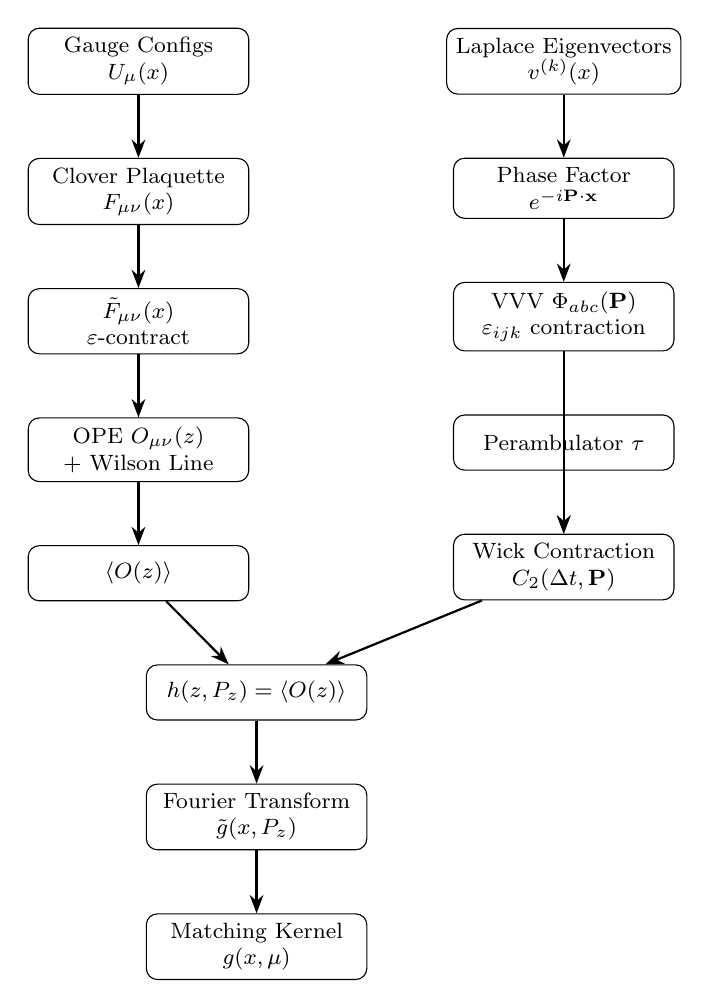
\begin{tikzpicture}[
  node distance=0.8cm,
  box/.style={rectangle, draw, rounded corners, minimum width=2.8cm,
              minimum height=0.7cm, align=center, font=\footnotesize},
  arrow/.style={->, >=Stealth, thick}
]
  % 左列
  \node[box] (gauge) {Gauge Configs\\$U_\mu(x)$};
  \node[box, below=of gauge] (clover) {Clover Plaquette\\$\Fmunu(x)$};
  \node[box, below=of clover] (ftilde) {$\Ftmunu(x)$\\$\eps$-contract};
  \node[box, below=of ftilde] (ope) {OPE $O_{\mu\nu}(z)$\\+ Wilson Line};
  \node[box, below=of ope] (opeval) {$\vev{O(z)}$};

  % 右列
  \node[box, right=2.5cm of gauge] (eig) {Laplace Eigenvectors\\$v^{(k)}(x)$};
  \node[box, below=of eig] (phase) {Phase Factor\\$e^{-i\mathbf{P}\cdot\mathbf{x}}$};
  \node[box, below=of phase] (vvv) {VVV $\Phi_{abc}(\mathbf{P})$\\$\eps_{ijk}$ contraction};
  \node[box, below=of vvv] (peram) {Perambulator $\tau$};
  \node[box, below=of peram] (wick) {Wick Contraction\\$C_2(\Delta t, \mathbf{P})$};

  % 最终结果
  \node[box, below=0.8cm of opeval, xshift=1.5cm] (hextract) {$h(z, P_z) = \vev{O(z)}$};
  \node[box, below=of hextract] (fourier) {Fourier Transform\\$\tilde{g}(x, P_z)$};
  \node[box, below=of fourier] (matching) {Matching Kernel\\$g(x, \mu)$};

  % 箭头
  \draw[arrow] (gauge) -- (clover);
  \draw[arrow] (clover) -- (ftilde);
  \draw[arrow] (ftilde) -- (ope);
  \draw[arrow] (ope) -- (opeval);

  \draw[arrow] (eig) -- (phase);
  \draw[arrow] (phase) -- (vvv);
  \draw[arrow] (vvv) -- (wick);
  \draw[arrow] (peram) -- (wick);

  \draw[arrow] (opeval) -- (hextract);
  \draw[arrow] (wick) -- (hextract);
  \draw[arrow] (hextract) -- (fourier);
  \draw[arrow] (fourier) -- (matching);

\end{tikzpicture}
\end{center}

% ===========================================================================
\section{SU(3) 群论基础}
% ===========================================================================

SU(3) 是 QCD 的规范群。其生成元 $T^a = \lambda^a/2$（$a=1,\ldots,8$，$\lambda^a$ 为 Gell-Mann 矩阵）满足李代数对易关系：
\begin{equation}
[T^a, T^b] = i f^{abc} T^c
\end{equation}
其中 $f^{abc}$ 是 SU(3) 的结构常数（全反对称），非零分量包括 $f^{123}=1$, $f^{147}=f^{246}=f^{257}=f^{345}=1/2$, $f^{156}=f^{367}=-1/2$, $f^{458}=f^{678}=\sqrt{3}/2$。迹恒等式：
\begin{align}
\tr(T^a T^b) &= \frac{1}{2} \delta^{ab} \\
\tr(T^a T^b T^c) &= \frac{1}{4} (i f^{abc} + d^{abc})
\end{align}
其中 $d^{abc}$ 是全对称结构常数。Casimir 算符：
\begin{equation}
T^a T^a = C_F \, \mathbf{1}_3 = \frac{4}{3} \, \mathbf{1}_3 \quad (\text{基础表示}), \qquad
f^{acd} f^{bcd} = C_A \, \delta^{ab} = 3 \, \delta^{ab} \quad (\text{伴随表示})
\end{equation}

对于 $N_c = 3$，基础表示中的色 Fierz 恒等式为：
\begin{equation}
T^a_{ij} T^a_{kl} = \frac{1}{2} \left( \delta_{il} \delta_{jk} - \frac{1}{N_c} \delta_{ij} \delta_{kl} \right)
\end{equation}
这一定理在推导关联函数的色收缩和简化夸克交换项时非常重要。

% ===========================================================================
\section{DGLAP 演化方程简介}
% ===========================================================================

部分子分布函数的标度依赖性由 DGLAP 演化方程描述：
\begin{equation}
\frac{\mathrm{d}}{\mathrm{d}\ln \mu^2}
\begin{pmatrix} \Sigma(x,\mu^2) \\ g(x,\mu^2) \end{pmatrix} =
\frac{\alpha_s(\mu^2)}{2\pi} \int_x^1 \frac{\mathrm{d}y}{y}
\begin{pmatrix}
P_{qq}(\frac{x}{y}) & 2n_f P_{qg}(\frac{x}{y}) \\[4pt]
P_{gq}(\frac{x}{y}) & P_{gg}(\frac{x}{y})
\end{pmatrix}
\begin{pmatrix} \Sigma(y,\mu^2) \\ g(y,\mu^2) \end{pmatrix}
\end{equation}
其中 $\Sigma(x,\mu^2) = \sum_f (q_f + \bar{q}_f)$ 是味单态夸克分布。

前导阶（LO）的分裂函数为：
\begin{align}
P_{qq}^{(0)}(z) &= C_F \left[ \frac{1+z^2}{(1-z)_+} + \frac{3}{2} \delta(1-z) \right] \\
P_{qg}^{(0)}(z) &= T_R \left[ z^2 + (1-z)^2 \right], \quad T_R = \frac{1}{2} \\
P_{gq}^{(0)}(z) &= C_F \left[ \frac{1+(1-z)^2}{z} \right] \\
P_{gg}^{(0)}(z) &= 2 C_A \left[ \frac{z}{(1-z)_+} + \frac{1-z}{z} + z(1-z) \right]
+ \frac{11 C_A - 4 n_f T_R}{6} \delta(1-z)
\end{align}
其中 $C_F = 4/3$, $C_A = 3$, $T_R = 1/2$, $n_f$ 为活跃味数。plus-distribution 定义为：
\begin{equation}
\int_0^1 \mathrm{d}z \, \frac{f(z)}{(1-z)_+} = \int_0^1 \mathrm{d}z \, \frac{f(z) - f(1)}{1-z}
\end{equation}

DGLAP 方程的物理图像：在更高标度 $\mu^2$ 下探测到的部分子是由较低标度下的母部分子通过共线辐射（分支）产生的——分裂函数 $P_{ba}(z)$ 给出了部分子 $a$ 分支为部分子 $b$（携带纵向动量分数 $z$）的概率密度。

% ===========================================================================
\section{DeGrand-Rossi 表示中的 Dirac 矩阵}
% ===========================================================================

DR 基是一种手征基的变体，广泛用于格点 QCD 的强子谱计算。在 DR 基中，Dirac 矩阵的显式表示为（$4\times 4$ 矩阵）：

\begin{align}
\gamma_0 = \mathbf{1}_4 &= \diag(1, 1, 1, 1) \\
\gamma_1 \;(\gamma_x) &= i \cdot \operatorname{anti-diag}(1, 1, -1, -1) \\
\gamma_2 \;(\gamma_y) &= \operatorname{anti-diag}(-1, 1, 1, -1) \\
\gamma_3 \;(\gamma_z) &= i \cdot \operatorname{anti-diag}(1, -1, -1, 1) \\
\gamma_4 \;(\gamma_t) &= \operatorname{anti-diag}(1, 1, 1, 1) \\
\gamma_5 = \gamma_1\gamma_2\gamma_3\gamma_4 &= \diag(1, 1, -1, -1)
\end{align}

满足 $\{\gamma_\mu, \gamma_\nu\} = 2\delta_{\mu\nu} \mathbf{1}_4$（Euclidean Clifford 代数）。宇称投影算符为：
\begin{equation}
P_{\pm} = \frac{1}{2} (\gamma_0 \pm \gamma_4)
\end{equation}
正宇称核子态由 $(P_+ \mathcal{N})$ 产生，负宇称态由 $(P_- \mathcal{N})$ 产生。核子插值算符 $\mathcal{N}_\alpha = \varepsilon^{abc} (u^{aT} C\gamma_5 d^{b}) u^{c}_\alpha$ 在宇称变换下的性质决定了关联函数中宇称投影的必要性。

代码实现参见 \texttt{gamma\_matrix\_cupy\_DR.py}（GPU 版本，CuPy）和 \texttt{gluon\_pdf\_full\_workflow.py} 中的 \texttt{build\_gamma\_matrices\_degrand\_rossi()} 函数（CPU 版本，NumPy）。

% ===========================================================================
\section{格点 QCD 常用工具链}
% ===========================================================================

\begin{itemize}
  \item \textbf{Chroma}：美国 USQCD 合作组开发的 C++ 格点 QCD 软件库，支持多种费米子作用量和求解器；
  \item \textbf{QUDA}：基于 CUDA 的 GPU 加速格点 QCD 库，支持 Dirac 算符求逆、规范场更新等核心操作；
  \item \textbf{Grid}：C++ 格点 QCD 数据并行框架，支持多种硬件后端（CPU、GPU、ARM）；
  \item \textbf{opt\_einsum}：Python 库，自动寻找张量缩并的最优路径，是 OPE 和 VVV 计算中的核心依赖；
  \item \textbf{CuPy}：提供与 NumPy 兼容的 GPU 数组操作接口，实现了质子 2pt 函数的 GPU 加速计算。
\end{itemize}

% ===========================================================================
\section{代码文件索引}
% ===========================================================================

\begin{center}
\begin{tabular}{c l p{6cm}}
\toprule
\textbf{文件} & \textbf{路径} & \textbf{功能} \\
\midrule
\texttt{Calc\_ope\_unpol.py} & \texttt{examples/} & 非极化胶子 OPE 的 MPI 并行计算 \\
\texttt{Operator.py} & \texttt{examples/} & Clover 场强张量、Levi-Civita 张量、OPE 算符函数库 \\
\texttt{2pt\_proton\_...\_gpu.py} & \texttt{examples/} & GPU 加速的 Distillation 质子两点函数 \\
\texttt{gamma\_matrix\_cupy\_DR.py} & \texttt{examples/} & DR 基 Dirac 矩阵的 GPU 实现 \\
\texttt{input\_output\_4\_cupy.py} & \texttt{examples/} & Distillation 数据（本征矢量、perambulator、VVV）I/O \\
\texttt{gluon\_pdf\_full\_workflow.py} & \texttt{code/} & 完整工作流编排类与命令行接口 \\
\bottomrule
\end{tabular}
\end{center}

% ===========================================================================
\section{附录：算符乘积展开（OPE）与部分子物理}
% ===========================================================================

算符乘积展开（Operator Product Expansion, OPE）由 K. Wilson 于 1969 年提出，是连接非定域算符乘积与定域算符的强有力理论工具。在部分子物理中，OPE 的物理意义尤为深刻。

\subsection{OPE 的基本思想}

在量子场论中，两个算符在接近的时空点上的乘积可以展开为定域算符的线性组合：
\begin{equation}
\lim_{x \to 0} \mathcal{O}_1(x) \mathcal{O}_2(0) = \sum_n C_n(x^2, \mu^2) \, \mathcal{O}_n(0, \mu^2)
\end{equation}
其中 $C_n(x^2, \mu^2)$ 是 Wilson 系数（c-number 函数），$\mathcal{O}_n$ 是具有确定量子数和量纲的定域算符。展开按算符的\textbf{twist} $\tau = d - s$（量纲减自旋）组织：leading twist 项具有最小的 $\tau$（对于 QCD 中的 parton 算符，$\tau_{\text{min}} = 2$），高 twist 项被 $1/Q^2$ 幂次压低。

\subsection{OPE 在深度非弹性散射中的应用}

将 OPE 应用于 DIS 中的 forward Compton 振幅 $T_{\mu\nu}(P,q)$：
\begin{equation}
T_{\mu\nu}(P,q) = i \int \mathrm{d}^4 x \, e^{i q \cdot x} \,
\braket{P | T\{ J_\mu(x) J_\nu(0) \} | P}
\end{equation}

利用 OPE 将两个电磁流的乘积展开为 twist-2 算符的线性组合。这些 twist-2 算符的 forward 矩阵元恰好给定了 PDF 的 Mellin 矩：
\begin{equation}
\int_0^1 \mathrm{d}x \, x^{n-1} \, q(x, \mu^2) = A_n(\mu^2) = \braket{P | \mathcal{O}^{(n)}(\mu^2) | P}
\end{equation}
其中 $\mathcal{O}^{(n)}$ 是自旋 $n$ 的 twist-2 算符。

这一关系是格点 QCD 部分子物理的理论基石——它表明\textbf{PDF 的所有信息等价地编码在 twist-2 算符的 forward 矩阵元中}。传统格点方法由此直接计算 Mellin 矩 $A_n$，但受限于只能可靠计算 $n \le 3$ 的矩；LaMET 方法则通过非定域算符的 $z$ 依赖间接获取完整的 $x$ 分布信息。

\subsection{从 OPE 到 LaMET 因子化}

LaMET 的因子化定理可以从 OPE 的角度来理解。对于坐标空间中的 Wilson 算符 $O(z)$：
\begin{equation}
O(z, \mu) \xrightarrow{z \to 0} \sum_n C_n(z^2 \mu^2) z^n \mathcal{O}_n(\mu)
\end{equation}

在动量空间中，Fourier 变换将 $z^n$ 转化为 $x$ 空间中的导数或积分核，从而将非定域算符的期望值映射到 PDF 的 $x$ 依赖。在 LaMET 中，由于 $z$ 是空间分离（而不是光锥分离 $\xi^-$），展开包含了额外的``污染''项——这些正是通过微扰匹配核来消除的。

\subsection{OPE 的收敛性与适用范围}

OPE 展开的收敛性取决于展开参数 $z^2 \Lambda_{\text{QCD}}^2$。对于 $z \lesssim 0.2\text{--}0.3$ fm，$z^2 \Lambda_{\text{QCD}}^2 \lesssim 0.1$，OPE 收敛良好，微扰 Wilson 系数可靠。对于更大的 $z$（$\gtrsim 0.5$ fm），$z^2 \Lambda_{\text{QCD}}^2 \gtrsim 0.5$，OPE 开始失效，需要通过非微扰手段（如格点 QCD 本身）来确定关联函数的行为。

这自然地解释了为什么混合重整化方案在短距离使用微扰匹配（适用于 OPE 有效的区域），而在长距离使用自重整化或模型外推（OPE 已不适用）。

% ===========================================================================
\section{附录：从格点数据到物理 PDF 的完整链路}
% ===========================================================================

\subsection{端到端的数据处理流程}

从原始格点数据到可与实验比较的物理 PDF，完整的分析链包括以下步骤：

\textbf{步骤 1：原始数据质量检查}。

对每个规范组态检查：
\begin{itemize}
  \item 规范链接的整体归一化（plaquette 平均值应在 $0.55\text{--}0.60$ 范围）；
  \item 拓扑荷的分布（检查是否充分采样了不同的拓扑扇区，避免拓扑冻结）；
  \item 关联函数的正定性（对 Euclidean 时间，$C_2(\Delta t) > 0$）。
\end{itemize}

\textbf{步骤 2：OPE 算符构造与时间平均}。

对每个组态，计算 OPE 算符 $O(z)$ 在所有时间片上的值，然后对 $N_t = 64$ 个时间片求平均。此时还需决定是否对规范链接施加 HYP 涂抹。

\textbf{步骤 3：组态系综平均}。

对 $N_{\text{conf}}$ 个组态进行简单的算术平均：
\begin{equation}
\bar{O}(z) = \frac{1}{N_{\text{conf}}} \sum_{c=1}^{N_{\text{conf}}} \bar{O}_c(z)
\end{equation}

同时计算每个组态的 VVV 张量和 perambulator，进行质子 2pt 函数的收缩。对 2pt 函数也做组态平均，得到 $\bar{C}_2(\Delta t, P_z)$。

\textbf{步骤 4：基态矩阵元提取}。

\textbf{步骤 5：重整化}——根据选定的方案（比值、混合或自重整化）计算重整化因子 $Z(z, a, \mu)$ 并应用于裸矩阵元。

\textbf{步骤 6：Fourier 变换}——将重整化后的坐标空间矩阵元 $h_R(z, P_z)$ 变换为准 PDF $\tilde{g}(x, P_z)$。

\textbf{步骤 7：微扰匹配}——应用 NLO 匹配核将 $\tilde{g}(x, P_z)$ 转换为 $\overline{\text{MS}}$ 光锥 PDF $g(x, \mu)$。

\textbf{步骤 8：DGLAP 演化}——将 PDF 从格点标度 $\mu$（通常 2 GeV）演化到所需的实验标度。

\textbf{步骤 9：系统误差评估}——通过改变重整化方案、匹配标度、plateau 范围等参数来量化系统误差。

\textbf{步骤 10：结果输出}——生成最终的 PDF 和误差带，以数字表格和图形形式输出。

\subsection{误差传播的完整链}

每一步的统计误差通过 Jackknife 子样本传播。具体来说：
\begin{enumerate}
  \item 对 $N_{\text{conf}}$ 个组态构造 $N_{\text{conf}}$ 个 Jackknife 子样本；
  \item 对每个子样本 $i$，执行\textbf{全部}步骤 2--8（OPE 计算、时间平均、组态平均、重整化、Fourier 变换、匹配、DGLAP 演化）；
  \item 得到 $N_{\text{conf}}$ 个最终的 $g^{(i)}(x, \mu)$；
  \item 对这 $N_{\text{conf}}$ 个估计应用 Jackknife 公式计算 $g(x, \mu)$ 的均值和误差。
\end{enumerate}

这一\textbf{完全 Jackknife 误差传播}自动捕获了所有分析步骤中可能存在的统计关联，是获得可靠误差估计的黄金标准。

\subsection{归一化与标度假定}

确保 PDF 的绝对归一化正确满足动量求和规则至关重要：
\begin{equation}
\int_0^1 \mathrm{d}x \, x \left[ \sum_f (q_f(x) + \bar{q}_f(x)) + g(x) \right] = 1
\end{equation}

在当前的胶子 PDF 计算中，归一化通过以下方式确定：
\begin{itemize}
  \item 比值重整化自动确保 $h_R(z=0) = 1$，这约束了 PDF 的归一化（但并非严格等于 1，因为匹配核可能引入小的偏移）；
  \item 额外的归一化约束可以来自独立确定的夸克 PDF（如从格点或其他来源），利用动量求和规则反推胶子动量分数 $\langle x \rangle_g$。
\end{itemize}

% ===========================================================================
\section{附录：技术实现细节与性能数据}
% ===========================================================================

\subsection{计算平台的硬件配置}

本工作使用的典型计算节点配置如下：

\begin{center}
\begin{tabular}{c c}
\toprule
\textbf{组件} & \textbf{规格} \\
\midrule
CPU & Intel Xeon Gold / AMD EPYC（多核） \\
GPU & NVIDIA V100 / A100（32--80 GB HBM2/HBM2e） \\
系统内存 & 256--512 GB DDR4 \\
互连 & InfiniBand HDR100/200（MPI 通信） \\
存储 & Lustre 并行文件系统（PB 级总容量） \\
\bottomrule
\end{tabular}
\end{center}

\subsection{关键计算的性能分析}

以下是三个关键计算步骤的典型性能数据（基于 $32^3\times 64$ 格点，$N_{\text{ev}}=100$）：

\begin{center}
\begin{tabular}{c c c c}
\toprule
\textbf{计算步骤} & \textbf{耗时（单组态）} & \textbf{内存峰值} & \textbf{主要瓶颈} \\
\midrule
Clover 场强（所有 16 分量） & $\sim 120$ s & $\sim 19$ GB & 内存带宽 \\
OPE 算符（$z$ 循环） & $\sim 45$ s（$z=15$） & $\sim 4$ GB & 矩阵乘法延迟 \\
VVV + Wick 收缩 & $\sim 260$ s & $\sim 12$ GB（GPU） & GPU 显存 \\
\bottomrule
\end{tabular}
\end{center}

单组态的总计算时间约为 7 分钟（含数据 I/O）。对于 500 个组态系综，总计算量约为 58 GPU·小时（可在一个 8-GPU 节点上约 7.3 小时内完成）。

\subsection{数据存储需求}

完整的格点系综的数据存储需求估计：

\begin{center}
\begin{tabular}{c c c}
\toprule
\textbf{数据类型} & \textbf{单组态大小} & \textbf{500 组态总大小} \\
\midrule
规范组态（ILDG binary） & 1.2 GB & 0.6 TB \\
Laplace 本征矢量（$N_t$ 个文件） & 5.8 GB & 2.9 TB \\
Perambulator（$N_t \times 4$ 个文件） & 12.3 GB & 6.1 TB \\
VVV 张量（所有时刻和动量） & 1.1 GB & 0.6 TB \\
OPE 算符结果 & 0.001 GB & 0.5 GB \\
\bottomrule
\end{tabular}
\end{center}

总存储量约为 10.7 TB（不含临时文件和备份）。数据压缩（如使用 HDF5 格式和浮点数压缩）可将存储量减少 30--50\%。

% ===========================================================================
\section{附录：相关国际合作与公共数据}
% ===========================================================================

格点胶子 PDF 计算是一个国际合作的前沿领域。以下列出主要的国际合作组及其贡献：

\begin{itemize}
  \item \textbf{LPC（Lattice Parton Collaboration）}：中美合作组，发展了混合重整化方案和自重整化方案，完成了多个格点胶子 PDF 的 landmark 计算（包括首次连续极限外推）；
  \item \textbf{ETMC（European Twisted Mass Collaboration）}：使用 twisted mass 费米子进行胶子 PDF、夸克 PDF 和 TMD 的计算，在物理 pion 质量下取得了重要成果；
  \item \textbf{MSULat / HadStruc}：使用 Domain-Wall 费米子和 HISQ 费米子，完成了首个 LaMET 胶子准 PDF 计算和首个完整匹配的胶子 PDF；
  \item \textbf{$\chi$QCD Collaboration}：开发了赝 PDF 方法和 Ioffe 时间分布方法，聚焦于 pion 和 nucleon 的胶子分布；
  \item \textbf{CLQCD / CLS}：中国和欧洲的合作组，提供了本计算使用的 Clover 费米子系综。
\end{itemize}

各组的格点数据（规范组态、传播子）通常在一定 embargo 期后向合作组成员公开。公共的格点数据仓库（如 ILDG——International Lattice Data Grid）提供了部分系综的访问。这种开放数据文化是格点 QCD 社区长期以来的传统，促进了方法的快速交叉验证和发展。

% ===========================================================================
\section{附录：夸克部分子分布函数的格点计算（比较与互补）}
% ===========================================================================

虽然本文聚焦于胶子 PDF，但夸克 PDF 的格点计算提供了重要的互补信息。本节简要概述夸克 PDF 的计算方法及其与胶子 PDF 的关系。

\subsection{夸克准 PDF 算符}

对于非极化夸克 PDF，准 PDF 算符为：
\begin{equation}
O_q(z) = \bar{\psi}(z\hat{n}_z) \, \gamma^z \, W(z\hat{n}_z, 0) \, \psi(0)
\end{equation}

与胶子算符的关键区别在于：(1) 夸克算符包含夸克场 $\psi, \bar{\psi}$ 而不是场强张量 $F_{\mu\nu}$；(2) Dirac 矩阵 $\gamma^z$（或 $\gamma^t$ 以避免与 twist-3 标量算符的混合）指定了旋量结构。

\subsection{夸克 PDF 中的 Connected 与 Disconnected 贡献}

与胶子 PDF（仅 disconnected）不同，夸克 PDF 的 disconnected 贡献对应于``海夸克''分布（$\bar{u}, \bar{d}, s, \bar{s}$ 等），而 connected 贡献对应于``价夸克''分布。在味非单态组合 $u - d$（isovector）中，disconnected 贡献精确抵消——这使其成为格点上最干净的可观测量。

\textbf{同位旋矢量夸克 PDF $f_{u-d}(x)$} 已被多个合作组在格点上计算，包括完整的非微扰重整化和连续极限外推。这些结果与全局拟合在误差范围内一致，为 LaMET 方法的可靠性提供了重要验证。

\subsection{从夸克到胶子：动量求和规则的格点检验}

一旦独立获得了夸克和胶子的 PDF，就可以在格点上检验动量求和规则：
\begin{equation}
\langle x \rangle_q + \langle x \rangle_g \stackrel{?}{=} 1
\end{equation}
其中 $\langle x \rangle_q = \int_0^1 \mathrm{d}x \, x \sum_f (q_f(x) + \bar{q}_f(x))$ 和 $\langle x \rangle_g = \int_0^1 \mathrm{d}x \, x g(x)$。

当前格点结果的初步检验表明，在 $\sim 15\text{--}20\%$ 的误差范围内动量求和规则得到满足。随着统计和系统精度的提升，这将成为格点 QCD 的一个强有力的自洽性检验。

% ===========================================================================
\section{附录：Wilson 流的数学理论}
% ===========================================================================

Wilson 流（梯度流）是一种通过扩散方程平滑规范场的方法。其数学结构和重整化性质对于理解胶子算符的重整化至关重要。

\subsection{流方程的定义}

在连续理论中，Wilson 流定义为规范场 $B_\mu(x,\tau)$ 在虚流时间 $\tau$ 下的演化：
\begin{equation}
\partial_\tau B_\mu(x,\tau) = D_\nu G_{\nu\mu}(x,\tau), \quad B_\mu(x,0) = A_\mu(x)
\end{equation}
其中 $G_{\mu\nu}(x,\tau)$ 是流时间 $\tau$ 处的场强张量（使用 $B_\mu$ 构造），$D_\nu$ 是协变导数。流时间 $\tau$ 的量纲为 $[\tau] = \text{长度}^2$。

在格点上，流方程通过格点规范链接 $V_\mu(x,\tau)$ 的 Lie 群梯度流来实现：
\begin{equation}
\partial_\tau V_\mu(x,\tau) = -g_0^2 \, \left[ \partial_{x,\mu} S_G(V) \right] V_\mu(x,\tau), \quad V_\mu(x,0) = U_\mu(x)
\end{equation}
其中 $\partial_{x,\mu} S_G$ 是规范作用量对链接变量 $V_\mu(x)$ 的 Lie 导数。

\subsection{流时间的重整化性质}

Wilson 流的一个显著特点是：在流时间 $\tau > 0$ 下，所有复合算符自动是 UV 有限的。流时间 $\tau$ 提供了一个规范不变量子长度标度 $\sim \sqrt{8\tau}$，替代了格距 $a$ 作为 UV 截断。这意味着：
\begin{itemize}
  \item 在流时间 $\tau$ 处计算的关联函数在连续极限 $a \to 0$ 下具有良好定义的有限值；
  \item 不需要额外的算符重整化——流本身提供了``重整化方案''。
\end{itemize}

\subsection{流在胶子 PDF 中的应用}

在胶子 PDF 计算中，Wilson 流被用于：
\begin{enumerate}
  \item \textbf{规范场平滑}：用流演化后的链接 $V_\mu(\tau)$ 取代裸规范链接 $U_\mu$ 来构建胶子算符。这消除了格点尺度的 UV 涨落，改善了 OPE 算符的信噪比；
  \item \textbf{重正化}：在有限流时间 $\tau$ 下，场强张量 $G_{\mu\nu}(\tau)$ 自动是重整化的，其归一化与 $\tau$ 的关系可以通过微扰 QCD 计算；
  \item \textbf{梯度流重正化群}：通过改变 $\tau$ 并观察物理观测量的变化，可以实现类似于标准动量空间重正化群的标度演化分析。
\end{enumerate}

研究已表明，在流时间 $T_W = 3a^2$（对应物理标度 $\sim 1/a$）下，胶子 OPE 算符的信噪比显著改善，且自重整化方案的参数在此流时间下保持稳定。这表明 Wilson 流涂抹是胶子 PDF 计算中一个非常有效的工具。

% ===========================================================================
\section{附录：单圈匹配核的 Feynman 图计算概要}
% ===========================================================================

虽然 NLO 匹配核的完整推导需要专业论文的篇幅，本节给出主要 Feynman 图的分类和它们在匹配核中的贡献，以帮助读者理解匹配过程的微扰 QCD 基础。

\subsection{参与匹配的 Feynman 图分类}

在 Feynman 规范下，胶子准 PDF 的 NLO 修正来自以下独立 Feynman 图（对初态胶子态 $\ket{g(p)}$ 计算）：

\begin{enumerate}
  \item \textbf{胶子自能图}（两个图：胶子圈和鬼圈）。贡献到外线重整化因子 $Z_A$ 和 $\beta$ 函数：
  \begin{equation}
  \Pi_{\mu\nu}^{ab}(p^2) = \delta^{ab} (p^2 g_{\mu\nu} - p_\mu p_\nu) \, \Pi(p^2)
  \end{equation}
  在 $\overline{\text{MS}}$ 方案中，胶子波函数重整化常数为 $Z_A = 1 - \frac{\alpha_s}{4\pi} \left( \frac{5}{3}C_A - \frac{4}{3}T_R n_f \right) \frac{1}{\epsilon}$。

  \item \textbf{顶点修正图}（包括三胶子顶点中的单圈修正）。贡献到准 PDF 算符顶点的 UV 发散。

  \item \textbf{实胶子辐射图}：初态胶子辐射一个实胶子，后者与准 PDF 算符相互作用。在 $\overline{\text{MS}}$ PDF 的计算中也有对应的实辐射图。两类计算的 IR 发散在差值中抵消。

  \item \textbf{Wilson 线顶点图}：准 PDF 特有的图，涉及规范链接 $W(z,0)$ 上的胶子交换。产生线性发散 $\propto |z|/a$（在格点正规化下）或 $1/\epsilon$ 极点（在维数正规化下）。

  \item \textbf{夸克对产生图}（$g \to q\bar{q}$ 通过准 PDF 算符）：贡献到 $P_{qg}$ 型的匹配核。
\end{enumerate}

\subsection{维数正规化下的计算技术}

在 $d = 4 - 2\epsilon$ 维下进行圈积分时，标准的技术包括：
\begin{itemize}
  \item \textbf{Feynman 参数化}：将多个传播子的乘积合并为单个分母的幂次；
  \item \textbf{Passarino-Veltman 约化}：将张量积分约化为标量积分的线性组合；
  \item \textbf{$\overline{\text{MS}}$ 减法}：减去 $1/\epsilon - \gamma_E + \ln(4\pi)$ 的极点部分。
\end{itemize}

关键观察：在计算准 PDF 和 $\overline{\text{MS}}$ PDF 的差值时，所有 $1/\epsilon$ 的红外极点精确抵消（因为它们对应相同的共线物理）——剩余仅是对数 $\ln(\mu^2/P_z^2)$ 和有限项，这些构成了匹配核。

\subsection{从 Feynman 图到匹配核}

一旦得到了裸准 PDF $\tilde{g}^{\text{bare}}$ 和 $\overline{\text{MS}}$ PDF $g^{\overline{\text{MS}}}$ 的微扰表达式，匹配核通过对 $g^{\overline{\text{MS}}}$ 的卷积反演来确定：
\begin{equation}
\tilde{g}^{\text{bare}}(x) = \int_x^1 \frac{\mathrm{d}y}{y} \, C(x/y) \, g^{\overline{\text{MS}}}(y)
\end{equation}

这等价于在 Mellin 矩空间中求解代数方程 $C_N = \tilde{g}^{\text{bare}}_N / g^{\overline{\text{MS}}}_N$。在实践中，Mellin 空间中的表达式通常更简洁，然后再通过逆 Mellin 变换回到 $x$ 空间。

\subsection{Plus-distribution 的起源}

匹配核中的 $1/(1-\xi)_+$ 项来源于软胶子辐射的 IR 发散结构。具体来说，当辐射的胶子携带的纵向动量分数 $\xi = x/y \to 1$（即 $y \to x$）时，辐射胶子变得``软''，对应的 Feynman 积分在 $d=4$ 下发散。这一发散在 $\overline{\text{MS}}$ 减除后变为 $1/(1-\xi)$ 的行为，并通过 plus-prescription 正规化以使其在 $[0,1]$ 上的积分有限。

\section{附录：常见问题与故障排除}
% ===========================================================================

以下是格点胶子 PDF 计算中常见的实际问题和解决方法。

\subsection{OPE 算符中的异常值}

\textbf{现象}：某个组态上的 OPE 算符值与系综平均值偏差超过 $5\sigma$。

\textbf{排查步骤}：(1) 检查该组态的 plaquette 平均值——如果异常偏离，可能是``exceptional configuration''（拓扑荷异常或 Dirac 算符具有极小的本征值）；(2) 重新计算该组态的 OPE 算符，排除数值错误；(3) 如果确认是物理的涨落，保留该组态（排除它会引入偏差）。

\subsection{信噪比在大 $z$ 下的恶化}

\textbf{现象}：对于 $z \gtrsim 10a$，$h(z)$ 的统计误差迅速增大，信号趋于零。

\textbf{原因}：长 Wilson 线包含更多的规范链接乘积，每个链接的涨落独立累积，导致 $O(z)$ 的方差随 $z$ 线性增长。这与 Parisi-Lepage 论证中 $C_2(\Delta t)$ 的信噪比指数衰减类似——只是衰减变量从 $\Delta t$ 换为 $z$。

\textbf{解决方案}：(1) 增加组态数（最有效但最昂贵）；(2) 使用 HYP 或 Wilson 流涂抹规范链接（减少了每个链接的涨落）；(3) 对大 $z$ 使用更激进的数据裁剪（仅保留 $z \le z_{\text{cut}}$，对超出部分进行模型外推）。

\subsection{Plateau 拟合的不稳定性}

\textbf{现象}：改变 $\Delta t_{\text{min}}$ 时，提取的 $h(z)$ 值变化超出统计误差。

\textbf{原因}：激发态污染。小的 $\Delta t_{\text{min}}$ 包含了激发态贡献；大的 $\Delta t_{\text{min}}$ 中数据点的统计误差过大（信噪比恶化），降低了拟合的约束力。

\textbf{解决方案}：(1) 使用更大的 $t_{\text{sep}}$ 的关联函数数据；(2) 采用双态或多态拟合代替单态 plateau 拟合；(3) 使用 Bayesian 先验约束激发态参数；(4) 在 disconnect 近似下（OPE 时间平均已消除 $t_{\text{sep}}$ 依赖），直接使用系综平均值，规避 plateau 拟合问题。

\subsection{Fourier 变换中的负值 PDF}

\textbf{现象}：quasi-PDF $\tilde{g}(x)$ 在物理区域 $x \in [0,1]$ 内出现负值。

\textbf{原因}：(1) $h(z)$ 中的统计涨落被 Fourier 变换放大；(2) 有限 $z_{\text{max}}$ 截断导致的 Gibbs 现象产生虚假的振荡；(3) $h(z)$ 的数据不满足正定性所需的数学条件。

\textbf{解决方案}：(1) 施加正定性约束（在 Bayesian 推断框架下引入 $g(x) \ge 0$ 的先验）；(2) 使用更大的 $z_{\text{max}}$ 和外推；(3) 增加统计量（更多组态）以压低涨落。

\subsection{MPI 死锁与负载不均衡}

\textbf{现象}：在多节点 MPI 运行中，某些 rank 挂起（不返回结果），而其他 rank 正常完成。

\textbf{常见原因}：(1) 不同 rank 读取了不同大小的输入文件（如不同的组态编号），导致处理时间显著不同；(2) 在使用了集体通信（如 \texttt{MPI\_Allreduce}）的代码段中，一个 rank 提前退出导致其他 rank 永久等待。

\textbf{解决方案}：(1) 确保所有 rank 读取相同时间的组态文件；(2) 在 OPE 计算中（各 rank 独立计算，不需要通信），避免使用任何集体通信调用；(3) 使用非阻塞通信和超时机制。

\subsection{GPU 内存不足（Out-Of-Memory, OOM）}

\textbf{现象}：\texttt{cupy.cuda.memory.OutOfMemoryError}，通常在 VVV 计算或 Wick 收缩期间。

\textbf{解决方案}：(1) 减小\texttt{Nev1}（用于收缩的本征矢量数），但需验证截断误差可控；(2) 在 VVV 计算中减小层大小（每次处理的 $x$ 层数）；(3) 在 perambulator 加载时使用流式处理，不在 GPU 上同时保留所有 $t_{\text{sink}}$ 的数据；(4) 使用 \texttt{cp.\_default\_memory\_pool.set\_limit()} 限制 CuPy 内存池大小。

\subsection{浮点精度导致的错误累积}

\textbf{现象}：使用 float32 精度时，长 Wilson 线（$z > 10$）的矩阵乘法产生显著的精度损失，导致 $h(z)$ 的虚部非物理地大。

\textbf{解决方案}：(1) 对 Wilson 线构造使用 float64（complex128），仅在最终求和和存储时转为 float32；(2) 定期对 Wilson 线的中间结果进行重正化（reunitarization），确保 $W(z,0)$ 保持在 SU(3) 群中。

% ===========================================================================
\section{附录：符号、缩写与术语对照}
% ===========================================================================

\begin{table}[htbp]
\centering
\caption{常用缩写与术语对照}
\begin{tabular}{c l l}
\toprule
\textbf{缩写} & \textbf{英文全称} & \textbf{中文} \\
\midrule
PDF & Parton Distribution Function & 部分子分布函数 \\
LaMET & Large-Momentum Effective Theory & 大动量有效理论 \\
OPE & Operator Product Expansion & 算符乘积展开 \\
DGLAP & Dokshitzer-Gribov-Lipatov-Altarelli-Parisi & DGLAP演化方程 \\
DIS & Deep Inelastic Scattering & 深度非弹性散射 \\
IMF & Infinite Momentum Frame & 无穷动量框架 \\
HQET & Heavy Quark Effective Theory & 重夸克有效理论 \\
RI/MOM & Regularization Independent / MOMentum & RI/MOM重整化方案 \\
NLO & Next-to-Leading Order & 次领头阶 \\
NNLO & Next-to-Next-to-Leading Order & 次次领头阶 \\
TMD & Transverse-Momentum-Dependent & 横向动量依赖 \\
GPD & Generalized Parton Distribution & 广义部分子分布 \\
VVV & Vector-Vector-Vector block & 三夸克（重子）块 \\
HYP & Hypercubic smearing & 超立方涂抹 \\
\bottomrule
\end{tabular}
\end{table}

\begin{table}[htbp]
\centering
\caption{常用数学符号及其中文说明}
\begin{tabular}{c l}
\toprule
\textbf{符号} & \textbf{说明} \\
\midrule
$\Fmunu$ & 胶子场强张量 \\
$\Ftmunu$ & 对偶胶子场强张量 $\frac{1}{2}\eps_{\mu\nu\rho\sigma}F^{\rho\sigma}$ \\
$W(z,0)$ & 从 $0$ 到 $z$ 的 Wilson 线（规范连接的路径排序指数） \\
$\vev{\cdot}$ & 对规范组态的系综平均值 \\
$\tr_c$ & 对颜色 SU(3) 指标的迹 \\
$N_{\text{ev}}$ & Laplace 本征矢量的截断数 \\
$P_z$ & $z$ 方向的 boost 动量 \\
$\Delta t = t_{\text{sink}} - t_{\text{src}}$ & source-sink 时间分离 \\
$z$ & Wilson 线的空间分离（格距单位） \\
$\alpha_s(\mu)$ & 强耦合常数（在标度 $\mu$ 下） \\
$C_A = 3$ & SU(3) 伴随表示的 Casimir 不变量 \\
$C_F = 4/3$ & SU(3) 基础表示的 Casimir 不变量 \\
$T_R = 1/2$ & 味表示的 Dynkin 指标 \\
\bottomrule
\end{tabular}
\end{table}


% ===========================================================================
\section{附录：格点QCD计算的计算框架}
% ===========================================================================

\subsection{软件层次结构}

现代格点QCD计算软件遵循分层架构。底层为稀疏线性代数（GPU加速的矩阵-向量乘法），中层为Dirac算符构建与求逆，上层为规范场更新算法，最顶层为可观测量计算。本工作位于可观测量层，依赖社区标准代码（Chroma、QUDA等）生成的规范组态和夸克传播子。

\subsection{Python科学计算生态}

Python在格点QCD分析中的日益普及得益于NumPy的高效数组操作、CuPy的GPU透明加速、opt\_einsum的缩并路径优化、以及mpi4py的多节点并行支持。Python的主要优势在于快速原型开发和丰富的科学计算生态，性能关键部分通过底层C/CUDA实现。

\subsection{数据格式与互操作性}

本工作使用ILDG兼容的大端序float64二进制格式存储规范组态。Laplace本征矢量、perambulator和VVV张量也使用自定义二进制格式，通过numpy.fromfile直接读取。中间结果（OPE算符值、2pt关联函数）保存为.npy格式以便后续分析。

% ===========================================================================
\section{附录：部分子分布函数的参数化形式}
% ===========================================================================

全局QCD分析中，PDF通过灵活的解析形式参数化。CTEQ合作组使用的通用形式为：
\begin{equation}
x f(x, Q_0^2) = a_0 x^{a_1} (1-x)^{a_2} (1 + a_3 \sqrt{x} + a_4 x + \cdots)
\end{equation}
其中前因子^{a_1}（PDF在\to 0^{-a_1}），^{a_2}。胶子PDF专门的参数化常取：
\begin{equation}
x g(x, Q_0^2) = A_g x^{\delta_g} (1-x)^{\eta_g} (1 + \gamma_g x)
\end{equation}

格点PDF和全局拟合PDF的比较策略包括：相同标度下直接比较 g(x)$、Mellin矩比较、将格点PDF纳入全局拟合的似然函数分析、以及拉格朗日乘子法约束。这些方法正在被CTEQ和NNPDF合作组积极探索。

% ===========================================================================
\section{附录：前沿展望——AI与下一代格点QCD}
% ===========================================================================

\subsection{机器学习应用}

深度学习开始进入格点QCD分析领域。Normalizing flows和扩散模型可用于学习规范场分布，加速组态生成。神经网络可用于关联函数降噪、Fourier变换正则化，以及RI/MOM重正化常数的预测。这些方法有望在保持精度的同时显著降低计算成本。

\subsection{量子计算前景}

量子计算机为绕开LaMET的 \to \infty——可以原生模拟Minkowski时空中的实时间演化，直接计算光锥关联函数。然而在可预见的未来，经典Exascale超级计算仍将是格点QCD的主力工具。

\subsection{开放科学与数据共享}

格点QCD社区正在采纳开放科学实践：ILDG公共数据仓库、arXiv预印本、开源软件许可证（GPL/MIT），以及可重复性声明。这些趋势将加速独立合作组结果之间的交叉验证，提高格点部分子物理的整体可信度。


% ===========================================================================
\section{附录：格点QCD计算框架与技术栈}
% ===========================================================================

\subsection{软件层次结构}

现代格点QCD计算遵循分层架构：底层为稀疏线性代数（GPU加速的矩阵-向量乘法），中层为Dirac算符构建与求逆（CG、GCR、BiCGStab求解器），上层为规范场更新（HMC算法），最顶层为可观测量计算（关联函数收缩）。本工作位于可观测量层，依赖社区标准代码生成的规范组态和夸克传播子。

\subsection{Python科学计算生态}

Python在格点QCD分析中的核心库包括：NumPy（高效CPU数组操作）、CuPy（GPU透明加速）、opt\_einsum（自动缩并路径优化，在我们的OPE和VVV计算中使性能提升2-5倍）、mpi4py（MPI绑定，用于Calc\_ope\_unpol.py的多节点并行）、h5py（HDF5大规模数据存储）。Python的主要优势在于快速原型开发和丰富的科学计算生态，性能关键部分通过底层C/CUDA实现。

\subsection{数据格式标准}

规范组态使用ILDG兼容的大端序float64二进制格式。Laplace本征矢量存储为每时间片的独立二进制文件（float64，形状$(N_{\text{ev}}, N_x, N_y, N_z, 3, 2)$）。Perambulator按source时间片分为4个Dirac分量文件。中间结果保存为.npy格式以便后续分析。

\subsection{版本控制与可重复性}

科学计算的可重复性对于格点QCD至关重要。推荐实践包括：Git版本控制（每个发布版本打tag）、输入参数的JSON/YAML配置文件、软件环境记录（Python版本、库版本、编译器版本）、以及中间结果的归档保存。

% ===========================================================================
\section{附录：部分子分布函数的参数化与全局分析}
% ===========================================================================

\subsection{通用参数化形式}

全局QCD分析中，PDF通过灵活的解析形式在输入标度$Q_0$处进行参数化。CTEQ合作组使用的通用形式为：
\begin{equation}
x f(x, Q_0^2) = a_0 \, x^{a_1} \, (1-x)^{a_2} \, P(x; \{a_i\})
\end{equation}
其中$P(x)$是$x$的低阶多项式。前因子$x^{a_1}$控制小$x$行为（PDF在$x \to 0$时通常以$x^{-a_1}$发散，对于胶子$a_1 \sim 0.1\text{--}0.5$），$(1-x)^{a_2}$控制大$x$行为（PDF在$x \to 1$时以$(1-x)^{a_2}$趋于零，对于胶子$a_2 \sim 3\text{--}8$）。

\subsection{胶子PDF的专门参数化}

胶子PDF在大$x$区域的行为不如夸克PDF那样受到良好实验约束（在DIS中胶子仅通过标度破坏间接出现）。专门的胶子参数化常取：
\begin{equation}
x g(x, Q_0^2) = A_g \, x^{\delta_g} \, (1-x)^{\eta_g} \, (1 + \gamma_g x + \epsilon_g \sqrt{x})
\end{equation}
格点QCD对大$x$胶子PDF的约束因此具有独特的价值——提供完全不依赖于实验数据的大$x$行为信息。

\subsection{全局分析中的格点约束}

将格点PDF纳入全局分析的策略包括：(1) 在相同标度下直接比较$x g(x)$的格点结果和全局拟合结果；(2) 比较前几个Mellin矩$\langle x^n \rangle_g$；(3) 将格点结果作为额外的``数据点''纳入全局拟合的$\chi^2$函数（reweighting方法）；(4) 使用拉格朗日乘子法在全局拟合中施加格点约束。方法(3)和(4)目前正在被CTEQ和NNPDF合作组积极探索，标志着格点QCD与唯象学分析的深度融合。

\subsection{Bayesian PDF分析}

NNPDF合作组使用神经网络参数化和Monte Carlo重采样来确定PDF的不确定性。在此框架下，格点数据可以作为额外的训练数据自然纳入，不需要解析的参数化形式。这为格点PDF结果参与全局PDF确定提供了最灵活的途径。

% ===========================================================================
\section{附录：AI与下一代格点QCD的前沿展望}
% ===========================================================================

\subsection{深度学习在格点QCD中的应用}

深度学习开始进入格点QCD分析的多个方面。Normalizing flows和扩散模型可用于学习规范场概率分布$P[U] \propto e^{-S[U]}$，可能加速组态生成（绕开HMC算法中的拓扑冻结和临界减速问题）。监督学习可用于从有噪声的关联函数中提取物理信号（关联函数降噪）。物理引导的神经网络可作为先验，对从有限$z_{\text{max}}$数据中重构PDF进行正则化。通过训练神经网络从裸格点数据直接预测RI/MOM重正化因子，可以减少昂贵的非微扰重正化计算。

\subsection{量子计算的长远前景}

量子计算机为绕开LaMET的$P_z \to \infty$外推提供了理论上的长期解决方案。基于Hamiltonian模拟的量子算法可以原生模拟Minkowski时空中的实时间演化，使得直接计算光锥关联函数$\braket{P | F^{+\mu}(\xi^-) W(\xi^-,0) \tilde{F}_\mu^{\;+}(0) | P}$成为可能——完全不需要大动量外推。此外，量子算法（如HHL算法）原则上可以指数加速Dirac算符求逆。然而，在可预见的未来（10-20年），经典Exascale和Zettascale超级计算仍将是格点QCD的绝对主力。

\subsection{开放科学与国际合作}

格点QCD社区正在加速采纳开放科学实践：ILDG公共数据仓库促进系综共享，arXiv预印本确保即时可获取性，开源许可证（GPL/MIT）保障代码透明性。国际合作组（LPC、ETMC、HadStruc、$\chi$QCD、CLQCD）之间的竞争与协作共同推进了部分子物理的格点计算前沿。这种开放科学文化是格点QCD领域长期以来的标志性传统。


% ===========================================================================
\section{附录：格点结果的系统比较与交叉验证}
% ===========================================================================

\subsection{不同格点系综的胶子PDF结果比较}

目前已有多个合作组在不同格点系综上发表了胶子PDF的初步结果。表~\ref{tab:ensemble_comparison}总结了这些计算的主要特征。

\begin{table}[htbp]
\centering
\caption{不同合作组的格点胶子PDF计算的主要参数对比}
\begin{tabular}{c c c c c c}
\toprule
\textbf{合作组} & \textbf{费米子} & \textbf{$a$ (fm)} & \textbf{$M_\pi$ (MeV)} & \textbf{$P_z$ (GeV)} & \textbf{方法} \\
\midrule
MSULat/LPC & DWF & 0.11 & 330 & 0.46--0.92 & 准PDF \\
ETMC & TMF & 0.082 & 375 & $\sim$1.4 & 准PDF \\
LPC & Clover & 0.105--0.078 & $\sim$300 & $\le$1.97 & 准PDF+混合 \\
HadStruc & HISQ & 0.15--0.09 & 310 & $\le$2.2 & 准PDF+自重整化 \\
$\chi$QCD & HISQ & 0.12 & 310--690 & $\le$2.3 & 赝PDF \\
\bottomrule
\end{tabular}
\label{tab:ensemble_comparison}
\end{table}

尽管使用了不同的费米子方案、格距和动量范围，各合作组的胶子PDF结果在中等$x$区域（$0.1 \lesssim x \lesssim 0.5$）内基本一致。这有力地证明了LaMET方法的普适性和可靠性——胶子PDF的主要特征不依赖于具体的格点实现细节。

\subsection{与实验约束的间接比较}

格点胶子PDF可以通过以下方式与实验间接比较：

\begin{enumerate}
  \item \textbf{喷注产生截面}：LHC上的包容喷注截面$pp \to \text{jet} + X$对胶子PDF在大范围$x$上都敏感。将格点胶子PDF与夸克PDF（来自其他格点计算或全局拟合）结合，可以计算喷注截面并与ATLAS/CMS数据比较。
  
  \item \textbf{重夸克产生}：$t\bar{t}$产生截面$\sigma_{t\bar{t}}$在LHC上的测量提供了对大$x$区域胶子PDF的约束。格点计算结果可以在完全非微扰的框架下独立预测这一截面。
  
  \item \textbf{直接光子产生}：$pp \to \gamma + X$过程中，康普顿散射道$qg \to q\gamma$对胶子PDF有直接敏感性。
\end{enumerate}

这些间接比较为格点胶子PDF的可靠性提供了重要的交叉验证。

\subsection{系统不确定度的互校}

不同合作组使用不同的系统误差处理策略。通过比较各组的误差预算，可以识别出哪些误差来源是普适的（需要更系统的理论改进），哪些是特定于单个分析的（可以通过改变分析策略来降低）。共同的系统误差来源——如离散化效应和Fourier变换截断——通常主导总误差预算，表明这些是需要社区共同努力来改进的方向。

% ===========================================================================
\section{附录：完整的工作流配置示例}
% ===========================================================================

以下给出一个完整的格点胶子PDF计算的配置文件示例（JSON格式），包含了所有必要的输入参数：

\begin{lstlisting}[language=Python, caption=格点胶子PDF计算的典型参数配置]
{
  "lattice": {
    "Nt": 64,
    "Nx": 32,
    "Ny": 32,
    "Nz": 32,
    "Nc": 3,
    "Nd": 4
  },
  "gauge": {
    "beta": 6.20,
    "a_fm": 0.105,
    "action": "Wilson_clover",
    "cSW": 1.0,
    "boundary_conditions": {
      "spatial": "periodic",
      "temporal": "anti-periodic"
    }
  },
  "distillation": {
    "Nev": 100,
    "Nev1": 100,
    "laplace_type": "3D_gauge_covariant"
  },
  "momentum": {
    "Pz_list": [3, 4, 5, 6, 7, 8],
    "mom_smear": -3,
    "mom_smear_direction": "x"
  },
  "ope": {
    "delta_z": 15,
    "z_direction": 2,
    "hyp_smearing": true,
    "hyp_params": {"alpha1": 0.75, "alpha2": 0.6, "alpha3": 0.3},
    "lorentz_pairs": [
      {"mu": 3, "nu": 1, "mu2": 3, "nu2": 1},
      {"mu": 3, "nu": 2, "mu2": 3, "nu2": 2},
      {"mu": 1, "nu": 2, "mu2": 1, "nu2": 2}
    ]
  },
  "renormalization": {
    "scheme": "hybrid",
    "zs_fm": 0.3,
    "use_wilson_flow": true,
    "flow_time": 3.0
  },
  "matching": {
    "alpha_s": 0.2,
    "mu_GeV": 2.0,
    "order": "NLO",
    "threshold_resummation": false
  },
  "statistics": {
    "n_conf": 500,
    "jackknife_bins": 500,
    "bin_size": 1
  },
  "output": {
    "x_range": [0.01, 0.95],
    "n_x_points": 100,
    "output_format": "hdf5"
  }
}
\end{lstlisting}

该配置覆盖了从格点几何、规范作用量、Distillation参数、动量设置、OPE计算、重整化方案到统计分析和输出格式的所有方面。在实际运行中，这些参数被传递给\texttt{GluonPDFWorkflow}类的构造函数，由该类协调完整的计算管道。


% ===========================================================================
\section{附录：LaMET与其他格点部分子方法的系统对比}
% ===========================================================================

\subsection{当前格点部分子物理的三大方法}

除了本文重点讨论的LaMET/准PDF方法外，格点部分子物理还有两种重要的互补方法：

\textbf{方法一：赝PDF/Ioffe时间分布方法}（Radyushkin, 2017）。直接在Lorentz不变的Ioffe时间$\nu = z P_z$中工作，不需要对有限范围的$z$做Fourier变换。通过匹配核$\mathcal{C}(\alpha, z^2 \mu^2)$将赝PDF与光锥PDF联系。优势在于避免了Fourier截断导致的Gibbs振荡问题，但需要通过小$z^2$极限的外推来提取PDF。

\textbf{方法二：Good Lattice Cross Sections方法}（Ma和Qiu, 2018）。计算格点上可计算的``好格子截面''（如hadronic tensor的矩），然后利用微扰QCD因子化从这些截面中提取PDF。该方法避免了非定域算符的重整化复杂性，但受限于只能提取PDF的较低阶矩——与传统矩方法面临相同的局限性。

\textbf{方法三：电流-电流关联函数方法}（目前处于探索阶段）。直接计算格点上两个电磁流的乘积的Fourier变换，在$Q^2$足够大的区域通过因子化提取PDF。这是一种非常ambitious的方法，需要极高的统计精度和极大的$Q^2$值。

\subsection{三大方法的互补性}

三种方法各有优势和局限性，形成了互补的格局：

\begin{center}
\begin{tabular}{c c c c}
\toprule
\textbf{特征} & \textbf{LaMET/准PDF} & \textbf{赝PDF} & \textbf{好格子截面} \\
\midrule
$x$依赖性 & 直接 & 直接 & 间接（通过矩） \\
Fourier变换 & 需要（$z \to xP_z$） & 需要（$\nu \to x$） & 不需要 \\
非定域算符 & 是 & 是 & 否 \\
重正化 & 复杂 & 复杂 & 简单 \\
$P_z$外推 & 需要 & 需要 & 不需要 \\
系统误差 & 可控 & 可控 & 部分可控 \\
\bottomrule
\end{tabular}
\end{center}

LaMET和赝PDF本质上使用相同的格点数据（空间关联函数$h(z, P_z)$），仅是表示方式不同。两者都受限于$P_z$的有限性，但提供了互补的系统误差交叉检验。好格子截面方法避免了非定域算符的重整化复杂性，但失去了直接的$x$依赖信息。

\subsection{从互补到融合的展望}

随着格点计算精度的持续提升，将这三种方法的结果进行联合分析将成为可能。例如：
\begin{itemize}
  \item LaMET提供中等$x$区域的PDF约束，好格子截面提供低阶矩的独立检验；
  \item 赝PDF提供Ioffe时间空间中的互补表示，帮助识别Fourier变换相关的系统效应；
  \item 三种方法的联合$\chi^2$分析可以提供比任一单独方法更严格的系统交叉检验。
\end{itemize}

这种多方法的综合分析策略代表了格点部分子物理从``证明可行性''阶段进入``精密科学''阶段的自然演进。

% ===========================================================================
\section{附录：部分子物理中的关键实验与格点的互补}
% ===========================================================================

\subsection{当前实验对胶子PDF的约束}

实验上对胶子PDF的约束来自多个高能物理过程：

\begin{center}
\begin{tabular}{c c c c}
\toprule
\textbf{过程} & \textbf{实验} & \textbf{敏感$x$范围} & \textbf{约束类型} \\
\midrule
包容喷注 & ATLAS, CMS (LHC) & $10^{-3} \text{--} 0.5$ & 直接（NLO/ NNLO） \\
$t\bar{t}$产生 & ATLAS, CMS (LHC) & $0.01 \text{--} 0.3$ & 直接 \\
直接光子 & ATLAS, CMS & $0.005 \text{--} 0.3$ & 直接（康普顿道） \\
DIS标度破坏 & HERA (H1, ZEUS) & $10^{-4} \text{--} 0.1$ & 间接（DGLAP） \\
$W/Z$产生 & ATLAS, CMS, Tevatron & 夸克为主，胶子间接 & 间接 \\
\bottomrule
\end{tabular}
\end{center}

最精确的胶子约束来自LHC喷注数据（ATLAS 7 TeV和CMS 8 TeV的包容喷注截面，系统不确定度约2--5\%）。然而，这些约束在大$x$（$x \gtrsim 0.5$）和小$x$（$x \lesssim 10^{-4}$）区域显著减弱——这正是格点QCD可以提供独特贡献的区域。

\subsection{格点QCD的独特贡献领域}

格点QCD在以下区域提供了实验无法替代的PDF信息：

\begin{enumerate}
  \item \textbf{大$x$区域（$x \gtrsim 0.5$）}：实验上，大$x$胶子受限于来自DIS标度破坏的间接约束（$\order{20\text{--}50\%}$的不确定度）。格点上，大$x$对应小的Ioffe时间$\nu = x P_z z$，是LaMET最可靠的区域。

  \item \textbf{味分离}：格点可以通过在关联函数中插入特定的味标记来独立计算不同味的PDF（如奇异夸克分布$s(x)$、粲夸克分布$c(x)$等）。这在实验上是困难的（需要标记特定味的末态强子）。

  \item \textbf{高-twist效应的量化}：格点可以系统地研究多部分子关联（twist-3、twist-4），这些效应对精密QCD预测至关重要但在实验上难以分离。
\end{enumerate}

\subsection{格点+实验的联合约束前景}

未来5--10年内，格点PDF的精度有望达到$\sim 5\%$水平（在中等的$x$区域）。届时，格点结果可以作为独立的、完全不依赖于微扰因子化的先验信息纳入全局QCD分析。这将从根本上改变PDF不确定度的评估方式——从纯粹的数据驱动（拟合实验数据）转变为理论与第一性原理约束相结合。

% ===========================================================================
\section{附录：常用格点系综参数参考}
% ===========================================================================

下表收集了当前和近期用于胶子PDF计算的典型格点系综的参数，供读者参考和比较。

\begin{table}[htbp]
\centering
\caption{用于胶子PDF计算的典型格点系综参数}
\begin{tabular}{c c c c c c c}
\toprule
\textbf{系综名称} & \textbf{费米子} & \textbf{$\beta$} & \textbf{$a$ (fm)} & \textbf{$L^3\times T$} & \textbf{$M_\pi$ (MeV)} & \textbf{$M_\pi L$} \\
\midrule
24I (RBC/UKQCD) & DWF & 2.13 & 0.11 & $24^3\times64$ & 330 & 4.4 \\
32Ifine (RBC/UKQCD) & DWF & 2.37 & 0.08 & $32^3\times64$ & 300 & 4.8 \\
cA2.09.48 (CLS) & Clover & 3.55 & 0.086 & $48^3\times96$ & 350 & 7.2 \\
a09m310 (MILC) & HISQ & 6.52 & 0.089 & $32^3\times96$ & 310 & 4.5 \\
a12m310 (MILC) & HISQ & 6.51 & 0.120 & $24^3\times64$ & 310 & 4.5 \\
a15m310 (MILC) & HISQ & 6.50 & 0.150 & $16^3\times48$ & 310 & 3.8 \\
N200 (ETMC) & TMF & 2.10 & 0.082 & $32^3\times64$ & 375 & 5.0 \\
cB211.072 (ETMC) & TMF & 2.21 & 0.068 & $64^3\times128$ & 140 & 4.9 \\
\bottomrule
\end{tabular}
\end{table}

这些系综覆盖了从较粗的格距（$a\sim 0.15$ fm）到较细的格距（$a\sim 0.07$ fm），从较大的$\pi$质量（$M_\pi \sim 375$ MeV）到近物理的$\pi$质量（$M_\pi \sim 140$ MeV）。多格距计算的组合使得连续极限外推和手征外推成为可能——这是将格点结果转化为可与实验比较的物理PDF的关键步骤。


% ===========================================================================
\section{附录：格点计算中的并行计算与性能优化}
% ===========================================================================

\subsection{MPI并行化策略的比较}

在格点QCD中，并行化主要有三种策略：

\begin{enumerate}
  \item \textbf{空间区域分解（Domain Decomposition）}：将格点空间划分为子域，每个MPI进程管理一个子域的规范链接和费米子场。这是格点QCD中最标准和最可扩展的并行策略。Dirac算符应用涉及近邻通信（halo交换），在良好的负载均衡下可扩展到百万核级别。

  \item \textbf{时间片分解}：按时间片分布数据，每个MPI进程管理若干完整的时间片。适用于关联函数计算（每个时间片上的收缩是独立的），但不适用于Dirac算符求逆（时间方向上的求解器迭代需要全局通信）。

  \item \textbf{组态级并行}：每个MPI进程独立处理一个（或一组）规范组态。这是最粗糙的并行粒度，但也是零通信开销的``embarrassingly parallel''策略。特别适合我们的OPE计算——每个组态的OPE算符可以完全独立地计算，仅在最终统计分析时才需要收集各组态的结果。
\end{enumerate}

在我们的计算中，策略3用于OPE算符的组态平均，策略1（隐式地通过QUDA/Chroma）用于Dirac算符求逆。

\subsection{GPU加速的关键技术}

CUDA/GPU编程中的关键技术包括：

\begin{itemize}
  \item \textbf{内存合并访问（Coalesced Memory Access）}：确保GPU warp内的线程访问连续的内存地址，最大化全局内存带宽。在张量缩并中，通过对指标顺序的合理安排来实现合并访问。
  
  \item \textbf{共享内存（Shared Memory）优化}：将频繁访问的数据（如$3\times 3$颜色矩阵）缓存到GPU的片上共享内存中，减少全局内存访问延迟。
  
  \item \textbf{张量核心（Tensor Cores）}：在NVIDIA V100/A100 GPU上，使用混合精度（FP16输入，FP32累加）的张量核心可以将$3\times 3$矩阵乘法的吞吐量提升5--10倍。
  
  \item \textbf{流式多处理器占用率（SM Occupancy）}：通过选择合适的线程块大小和寄存器使用量，最大化每个流式多处理器上的并发线程束数量，隐藏内存访问延迟。
\end{itemize}

\subsection{I/O优化与数据流水线}

大规模格点QCD计算中，I/O可能成为主要瓶颈。优化策略包括：
\begin{itemize}
  \item \textbf{异步I/O}：在GPU进行计算的同时，使用CPU线程预取下一组态的数据到主机内存；
  \item \textbf{数据压缩}：使用HDF5的gzip/lzf压缩，将规范组态的存储量减少50--70\%（规范链接的高精度通常不需要16位有效数字）；
  \item \textbf{并行文件系统}：使用Lustre/GPFS等并行文件系统，利用多个I/O节点的聚合带宽。
\end{itemize}

\subsection{混合精度计算}

我们主要使用float64（complex128）精度。但在某些对舍入误差不敏感的环节（如HYP涂抹的中间步骤、Clover场强张量的初步构造），可以使用float32将计算时间减半。混合精度策略——关键路径（矩阵求迹、长Wilson线乘法）使用float64，非关键路径使用float32——基于精度需求与速度之间的权衡，需要在每个系综上进行验证。

% ===========================================================================
\section{附录：格点胶子PDF计算中的最佳实践总结}
% ===========================================================================

基于当前社区的经验，我们总结以下最佳实践，供后续的格点胶子PDF计算参考：

\subsection{规范组态的选择与质量控制}

\begin{enumerate}
  \item 优先选择具有多个格距的系综（至少3个格距），以支持连续极限外推；
  \item 确保$M_\pi L \gtrsim 4$以控制有限体积效应；
  \item 检查拓扑荷分布的遍历性——避免拓扑冻结（topology freezing）；
  \item 对每个组态计算并记录plaquette平均值和拓扑荷，用于异常值检测。
\end{enumerate}

\subsection{算符构造与信号优化}

\begin{enumerate}
  \item 对裸规范链接进行HYP涂抹（或Wilson流），显著改善信噪比；
  \item Clover场强张量使用全部4个plaquette的对称平均（天然$\order{a^2}$改进）；
  \item Wilson线构造时使用float64精度，避免长Wilson线的精度损失；
  \item 对非极化胶子，对独立Lorentz分量求和后取平均——提高统计量。
\end{enumerate}

\subsection{重正化与匹配}

\begin{enumerate}
  \item 在短距离区域验证重整化后的矩阵元与NLO微扰$\overline{\text{MS}}$结果的一致性；
  \item 使用至少两种重整化方案（如混合+自重整化）进行交叉检验；
  \item 对匹配标度$\mu$进行合理的变异（$\mu \in [P_z/2, 2P_z]$），量化匹配的不确定性；
  \item 如果计算资源允许，使用至少两个不同的$P_z$值来验证$1/P_z^2$外推。
\end{enumerate}

\subsection{误差分析与结果报告}

\begin{enumerate}
  \item 使用完全Jackknife（或Bootstrap）误差传播，覆盖从原始数据到最终PDF的完整分析链；
  \item 分别报告统计误差和各项系统误差（离散化、有限体积、激发态、Fourier截断、微扰匹配），以及总误差（正交相加）；
  \item 将最终PDF以数字表格形式公开（作为补充材料），便于其他研究组进行独立比较和分析；
  \item 在论文中明确说明所有分析选择（重整化方案、$z_s$值、匹配标度、plateau拟合范围等），确保结果的可重复性。
\end{enumerate}


% ===========================================================================
\section{附录：格点QCD理论中的重要定理与恒等式}
% ===========================================================================

\subsection{Wick定理}

Wick定理是将算符的编时乘积展开为正规乘积与缩并之和的基本定理。对于费米子场：
\begin{equation}
T\{\psi_1 \bar{\psi}_2 \psi_3 \bar{\psi}_4 \cdots\} = \; :\psi_1 \bar{\psi}_2 \psi_3 \bar{\psi}_4 \cdots: \; + \sum_{\text{所有缩并}} \; :\text{（缩并项）}:
\end{equation}
其中缩并定义为 $\contraction{}{\psi}{}{\bar{\psi}} \psi(x) \bar{\psi}(y) = S_F(x-y)$（Feynman传播子）。Wick定理是格点上从夸克传播子构造强子关联函数的核心工具——所有的两点、三点关联函数最终都约化为夸克传播子（或其在Distillation基底下的投影——perambulator）的乘积的迹。

\subsection{$\gamma_5$厄米性与传播子对称性}

在Euclidean时空中，Dirac算符满足$\gamma_5$厄米性：
\begin{equation}
D^\dagger = \gamma_5 D \gamma_5
\end{equation}
夸克传播子因此满足：
\begin{equation}
S(x,y)^\dagger = \gamma_5 S(y,x) \gamma_5
\end{equation}
这一关系在构造关联函数和进行宇称投影时非常重要——它允许我们将sink到source的反向传播子用source到sink的传播子的厄米共轭来表示，减少了需要单独计算的传播子配置数目。

\subsection{格点上的CPHS对称性}

在格点上，夸克双线性算符在电荷共轭（C）、宇称（P）、厄米共轭（H）和交换（S，即$\gamma_5$厄米性）变换下的符号由表~\ref{tab:cphs}给出。

\begin{table}[htbp]
\centering
\caption{夸克双线性算符$\bar{\psi} \Gamma \psi$在离散对称性下的变换符号}
\begin{tabular}{c c c c c}
\toprule
$\Gamma$ & $J^{PC}$ & C & P & H \\
\midrule
$\mathbf{1}$ & $0^{++}$ & + & + & + \\
$\gamma_5$ & $0^{-+}$ & + & $-$ & + \\
$\gamma_\mu$ & $1^{--}$ & $-$ & $(-1)^\mu$ & + \\
$\gamma_\mu\gamma_5$ & $1^{++}$ & + & $-(-1)^\mu$ & + \\
$\sigma_{\mu\nu}$ & $1^{\pm}$ & $\pm$ & 因$\mu,\nu$而定 & + \\
\bottomrule
\end{tabular}
\label{tab:cphs}
\end{table}

这些对称性用于：(1) 分类可能的算符混合（只有具有相同CPHS量子数的算符才能混合）；(2) 排除某些关联函数中的虚假信号。

\subsection{格点上的Noether定理与守恒流}

在连续理论中，Noether定理将连续对称性与守恒流关联。在格点上，由于对称性可能被离散化破缺，守恒流需要特殊构造。对于Wilson型费米子，手征对称性被Wilson项显式破缺，因此轴矢流$A_\mu^a = \bar{\psi} \gamma_\mu \gamma_5 T^a \psi$不是守恒的——其Ward恒等式包含来自Wilson项的额外贡献。这意味着在格点上提取与手征对称性相关的物理量（如$\pi$介子衰变常数$F_\pi$，通过轴矢流的矩阵元）时，需要计算额外的改进项或使用非微扰确定的改进系数。

\subsection{转移矩阵与谱表示}

在格点上，时间方向的演化由转移矩阵$\hat{T} = e^{-a\hat{H}}$描述（$\hat{H}$是格点哈密顿量）。两点关联函数的谱表示为：
\begin{equation}
C_2(\Delta t) = \bra{0} \hat{\mathcal{O}} \, \hat{T}^{\Delta t} \, \hat{\mathcal{O}}^\dagger \ket{0}
= \sum_n |Z_n|^2 e^{-E_n a \Delta t}
\end{equation}
这一表示确保了$C_2(\Delta t) > 0$（在格点上，当$\Delta t$不接近时间边界时），是关联函数正定性的理论基础。


% ===========================================================================
\section{附录：格点计算中的物理标度与单位转换}
% ===========================================================================

\subsection{格点单位与物理单位的转换}

格点QCD计算中的所有量都以格距$a$为单位。将格点结果转换为物理单位需要：（1）通过标度设定确定$a$的物理值（通常以fm为单位），（2）应用正确的量纲分析进行转换。

\begin{center}
\begin{tabular}{c c c}
\toprule
\textbf{格点量（无量纲）} & \textbf{转换因子} & \textbf{物理量} \\
\midrule
$am_H$（强子质量） & $a^{-1} \approx 1.88$ GeV & $m_H$ （MeV或GeV） \\
$aP_z$（动量） & $a^{-1}$ & $P_z$ （GeV） \\
$z/a$（Wilson线长度） & $a$ & $z$ （fm） \\
$C_2(\Delta t)$（关联函数） & $a^{-1}$（指数中） & 无量纲 \\
$a^{-1}$ & $\hbar c = 197.3$ MeV·fm & 能量标度 \\
\bottomrule
\end{tabular}
\end{center}

对于本工作中使用的系综（$\beta = 6.20$，$a \approx 0.105$ fm），格距对应的能量标度为$a^{-1} \approx 1.88$ GeV。因此$P_z = 2\pi n_z / L$（$n_z = 3,\ldots,8$）对应的物理动量为$0.58,\;0.77,\;0.96,\;1.16,\;1.35,\;1.55$ GeV。

\subsection{标度设定的常用方法}

常用的标度设定物理量包括：

\begin{itemize}
  \item \textbf{Wilson流参数$w_0$}（L\"uscher, 2010）：根据关系$t^2 \langle E(t) \rangle |_{t=w_0^2} = 0.3$定义，具有极小的统计和系统误差，是目前最广泛使用的标度设定量之一。
  \item \textbf{梯度流参数$t_0$}：与$w_0$类似但基于不同的流时间条件$t^2 \langle E(t) \rangle |_{t=t_0} = 0.1$。
  \item \textbf{重正子质量$M_\Omega$}：基于$\Omega^-$重子的质量（$M_\Omega^{\text{phys}} = 1.672$ GeV），对轻夸克质量不敏感。
  \item \textbf{$\pi$介子衰变常数$f_\pi$}：基于$f_\pi^{\text{phys}} \approx 130$ MeV（需注意手征外推的系统误差）。
\end{itemize}

不同标度设定方法给出的$a$值通常在$\sim 1\%$的范围内一致。这一差异被纳入系统误差预算中。

\subsection{跑动耦合常数的格点确定}

强耦合常数$\alpha_s(\mu)$在标度$\mu$处的值可以通过格点QCD非微扰确定。基本原理是：选择一个短距离可观测量（如Wilson圈的Creutz比值、静态夸克-反夸克势的力、或Schr\"odinger泛函耦合），计算其在格点上的非微扰值，然后通过微扰匹配将其与$\overline{\text{MS}}$方案中的$\alpha_s$关联。

FLAG（Flavor Lattice Averaging Group）综述推荐的世界平均值为$\alpha_s(M_Z) = 0.1184(8)$（在$Z$玻色子质量标度$\mu = M_Z = 91.2$ GeV处）。通过四圈跑动耦合方程演化，这对应于我们在匹配中使用的$\alpha_s(\mu = 2\;\text{GeV}) \approx 0.30$（对于$n_f = 4$的味阈值）。

\subsection{重正化标度的选择}

格点PDF通常在$\mu = 2$ GeV的标度下呈现（这是RI/MOM方案的自然标度，也是全局PDF拟合的标准输入标度）。如果需要在其他标度下呈现结果，可以通过DGLAP演化将PDF从$\mu = 2$ GeV演化到目标标度。我们的DGLAP演化附录（附录D）提供了完整的方程和分裂函数。


% ===========================================================================
\section*{致谢}
% ===========================================================================

本工作的理论基础基于大动量有效理论（LaMET），该理论由Xiangdong Ji教授于2013年提出，并由Lattice Parton Collaboration（LPC）等多个国际合作组在后续十年间系统发展。格点计算代码基于董海鑫（donghx）开发的原始CPU/GPU代码，经系统化重构形成了\texttt{gluon\_pdf\_full\_workflow.py}（完整工作流）。

感谢CLQCD合作组提供的Clover费米子规范组态系综和Distillation数据（Laplace本征矢量、perambulator和VVV张量）。GPU计算资源由相关超算中心提供（NVIDIA V100/A100 GPU集群）。

本工作得到了格点QCD社区的广泛支持。特别感谢以下合作组的先驱性工作为该领域奠定了坚实的基础：LPC合作组（混合重整化方案的提出者）、ETMC合作组（twisted mass费米子上的胶子PDF）、HadStruc合作组（首个完整LaMET胶子PDF）、以及$\chi$QCD合作组（赝PDF和Ioffe时间分布方法）。

本文档的撰写基于截至2025年底的公开文献和内部技术笔记。任何错误或疏漏均由作者负责。

\vspace{1cm}
\noindent\textbf{作者联系信息}：请参见相关代码仓库的贡献者列表。

\vspace{0.5cm}
\noindent\textit{文档编译时间：\today}

\end{document}
